\chapter{Numerical Implementation}
\label{chap:Implementation}
\begin{chaptersummarybox}
	The SOLEDGE3X mesh is aligned with magnetic flux surfaces and uses a multi-domain decomposition to handle singularities at X-points. In the FVM approach, time integration is performed with an implicit-explicit scheme, where all collisional processes and the new Alfvénic and electron inertial dynamics are solved implicitly. To benefit from first-order spatial derivatives, the new fields $A_\parallel$ and $j_\parallel$ are defined on a poloidally and toroidally staggered grid. This setup requires new discrete operators to accommodate the divergence $\left|\grad\cdot X^{stg}\textbf{b}\right|_{col}$ of a staggered field onto a collocated grid and parallel gradients $\left|\textbf{b}\cdot\grad X^{col}\right|_{stg}$ of collocated fields onto the staggered grid for the electromagnetic vorticity equation, as well as a staggered-to-staggered perpendicular Laplacian operator $\left|\grad\cdot\grad_\perp X^{stg}\right|_{stg}$ for Ampère's law. With four staggered radial cell faces facing the X-point at once, Neumann boundary conditions are applied there. \\	
	The new Ampère's law is solved along with the vorticity equation in a coupled 3D system for $\Phi$ and $A_\parallel$:	
	\begin{align*}
		\begin{pmatrix}
			\nabla \cdot \left[ D_\perp \nabla_\perp \circ \right] + \nabla \cdot \left[ D_\parallel \nabla_\parallel \circ \mathbf{b} \right]  
			& \frac{\beta_0}{\delta_t} \nabla \cdot \left[ D_\parallel \circ \mathbf{b} \right] \\
			-D_\parallel \nabla_\parallel \circ &
			\frac{\beta_0}{\delta_t} D_\parallel \circ - \nabla \cdot \left[ \nabla_\perp \circ \right]
		\end{pmatrix}
		\begin{pmatrix}
			\Phi^{n+1} \\ A_\parallel^{n+1}
		\end{pmatrix} 
		= 
		\begin{pmatrix}
			\nabla \cdot \left[ D_t j^{n}_\parallel \mathbf{b} \right] + \text{RHS}^\Phi \\
			D_t j^{n}_\parallel + \text{RHS}^{A_\parallel}
		\end{pmatrix}& \\
		\text{with: } D_\perp = \frac{m_i n_i}{B^2 \delta_t}, D_\parallel = \frac{1}{\eta_\parallel + \mu}, D_t = \frac{\mu}{\eta_\parallel + \mu}, \text{ and } \mu = \frac{m_e}{(n_e \delta_t)} &
	\end{align*}	
	Electron inertia mitigates the anisotropy between perpendicular and parallel Laplacian operators, acting as a lower bound for resistivity $\eta_\parallel$, and significantly improves the condition number in high-temperature plasmas. However, coupling with $A_\parallel$ worsens the matrix condition. \\
	Flutter adds a radial component to the magnetic field, requiring adjustments to all parallel operators in the flux-aligned geometry. For advection, flutter is treated as an additional drift velocity. The off-diagonal terms in the vorticity system increase coupling between $\Phi$ and $A_\parallel$, raising computational costs. To ensure consistency, the discrete parallel Laplacian on $\Phi$ must match the combination of divergence with gradient operators. For parallel viscous forces and heat conductivity, a new discrete operator was developed to limit radial numerical diffusion, but solving these problems now requires a full-domain 3D solver, increasing the computational cost.
\end{chaptersummarybox}

\newpage

The SOLEDGE3X framework uses a finite-volume method (FVM) with an implicit-explicit time integration scheme and variable stepsize (VSIMEX)\cite{wang2008variable}. The second-order conservative FVM scheme associated with a 3rd-order WENO reconstruction and Donat, Marquina fluxes for a modified Riemann solver for the advection terms to handle both shocks and complicated smooth solution structures \cite{tamain2016tokam3x, Bufferand2021}. In turbulence simulations, we focus on timescales slower than the cyclotronic frequency $\omega_C$, allowing explicit time-stepping for advection, friction, pressure, and energy source terms. This multi-step method is implemented for orders 1 to 3, with the timestep updated to match a targeted CFL value.

Ionization/recombination processes, resistive and viscous effects from the Spitzer-Härm model, electron inertia, and Alfvén dynamics involve faster dynamics than the ion cyclotronic time, and would strongly restrict the timestep size. These terms are therefore solved implicitly. To reduce complexity, they can be decoupled and solved sequentially for density, parallel velocity, temperature, and the vorticity equation.

This chapter details the implementation of the new electromagnetic model in this implicit-explicit framework. Sec. \ref{sec:impl_geometry} gives an overview of the field-aligned meshing and curvilinear coordinate system. Sec. \ref{sec:impl_staggeredMesh} introduces the poloidally and toroidally staggered mesh for the new fields $A_\parallel$ and $j_\parallel$, with the necessary discrete operators. Sec. \ref{sec:impl_EMvorticity} discusses the new electromagnetic vorticity equation, solved implicitly on $\Phi$ and $A_\parallel$. Finally, Sec. \ref{sec:impl_flutter} addresses the impact of the radial magnetic field component from flutter on all parallel operators.


\section{Geometrical consideration}
\label{sec:impl_geometry}

\subsection{Coordinate system}
\label{ssec:Implementation_CoordinateSystem}
Let $R_0$ be the major radius on the magnetic axis and $(R, Z, \varphi)$ a fixed cylindrical coordinate system. The magnetic equilibrium is assumed to be toroidally symmetric and to encompass both closed and open flux surfaces with singularities at one or more X-points. The 2D equilibrium magnetic field $\mathbf{B}_{eq} = B_{eq} \mathbf{b}_{eq}$ is a combination of a toroidal field, $\mathbf{B}_{eq,\varphi}$, and a poloidal field, $\mathbf{B}_{eq,p}$, as described in Sec. \ref{ssec:intro_tokamakConfiguration}:

\begin{equation}
	\mathbf{B}_{eq} = \mathbf{B}_{eq,\varphi} + \mathbf{B}_{eq,p} = F \nabla{\varphi} + \nabla{\Psi} \times \nabla{\varphi}
\end{equation}

where $\varphi$ is the toroidal angle, $F$ a toroidal flux function, and $\Psi(R,Z)$ a poloidal flux function from which $\mathbf{B}_{eq,\varphi}$ and $\mathbf{B}_{eq,p}$ are respectively derived (see Sec. \ref{sec:intro_GradShafranov}). The iso-$\Psi$ surfaces are tangent to the magnetic field and $\Psi$ labels flux surfaces (one value for each flux surface). It is thus natural to define a curvilinear system of coordinates denoted $(\psi, \theta, \varphi)$. $\psi$ defines a radial coordinate based on the poloidal magnetic flux $\Psi$, which is by construction always perpendicular to a magnetic flux surface. $\theta$ denotes a curvilinear abscissa along the poloidal direction in the $(R, Z)$ plane that defines the poloidal plane, i.e., along iso-$\Psi$ surfaces and orthogonal to $\grad  \varphi$. \newline

In the base $(\boldsymbol{e}_{\psi}, \boldsymbol{e}_{\theta}, \boldsymbol{e}_{\varphi})$ associated with $(\psi, \theta, \varphi)$, the magnetic equilibrium field is written as:

\begin{equation}
	\boldsymbol{B}_{eq} = B_{eq,p} \frac{\boldsymbol{e}_{\theta}}{\vert \boldsymbol{e}_{\theta} \vert} + B_{eq,\varphi} \frac{\boldsymbol{e}_{\varphi}}{\vert \boldsymbol{e}_{\varphi} \vert}
\end{equation}



\subsection{Domain decomposition and mesh design}
\label{ssec:impl_meshDecomposition}
In order to keep a structured flux-surfaces aligned mesh for any magnetic equilibrium, the real domain is mapped into a Cartesian domain decomposed into multiple connected zones \cite{tamain2016tokam3x}. Each point of the domain is distinctly identified by the set of curvilinear coordinates $[\psi, \theta, \varphi]$ defined in Sec. \ref{ssec:Implementation_CoordinateSystem}. The domain is segmented along the toroidal coordinate $\varphi$, into $N_{\varphi}$ poloidal planes. Tables of data fields are provided for each subdomain. Ghost cells store the information on the neighborhood within a matrix that defines how these subdomains are connected to each other. Depending on the domain, these ghost cells contain either the values of the neighboring subdomains' fields or the values imposed by the boundary conditions. An example of the mesh and its zone decomposition is shown in Fig. \ref{fig:TCVzoneDecomposition}, where the X-point requires six zones. \newline

\begin{figure}[H]\centering
	\begin{subfigure}[c]{0.5\textwidth}
		\centering
		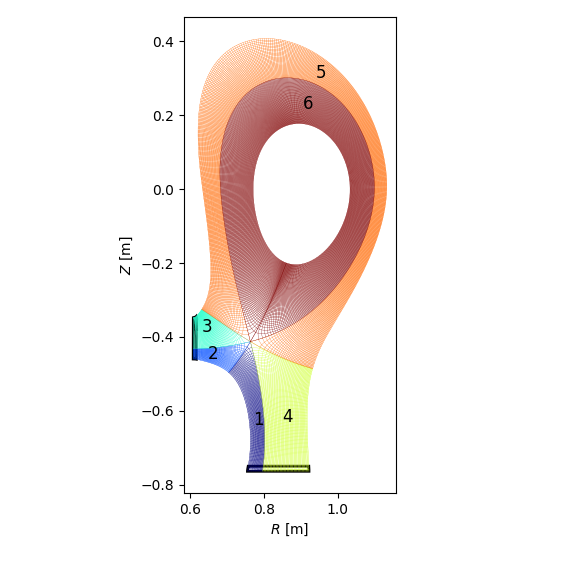
\includegraphics[width=1\textwidth]{schemes/TCVmesh.png}
		\subcaption{Typical mesh and zones decomposition}
		\label{fig:TCVmesh}
	\end{subfigure}
	\begin{subfigure}[c]{0.3\textwidth}
		\centering
		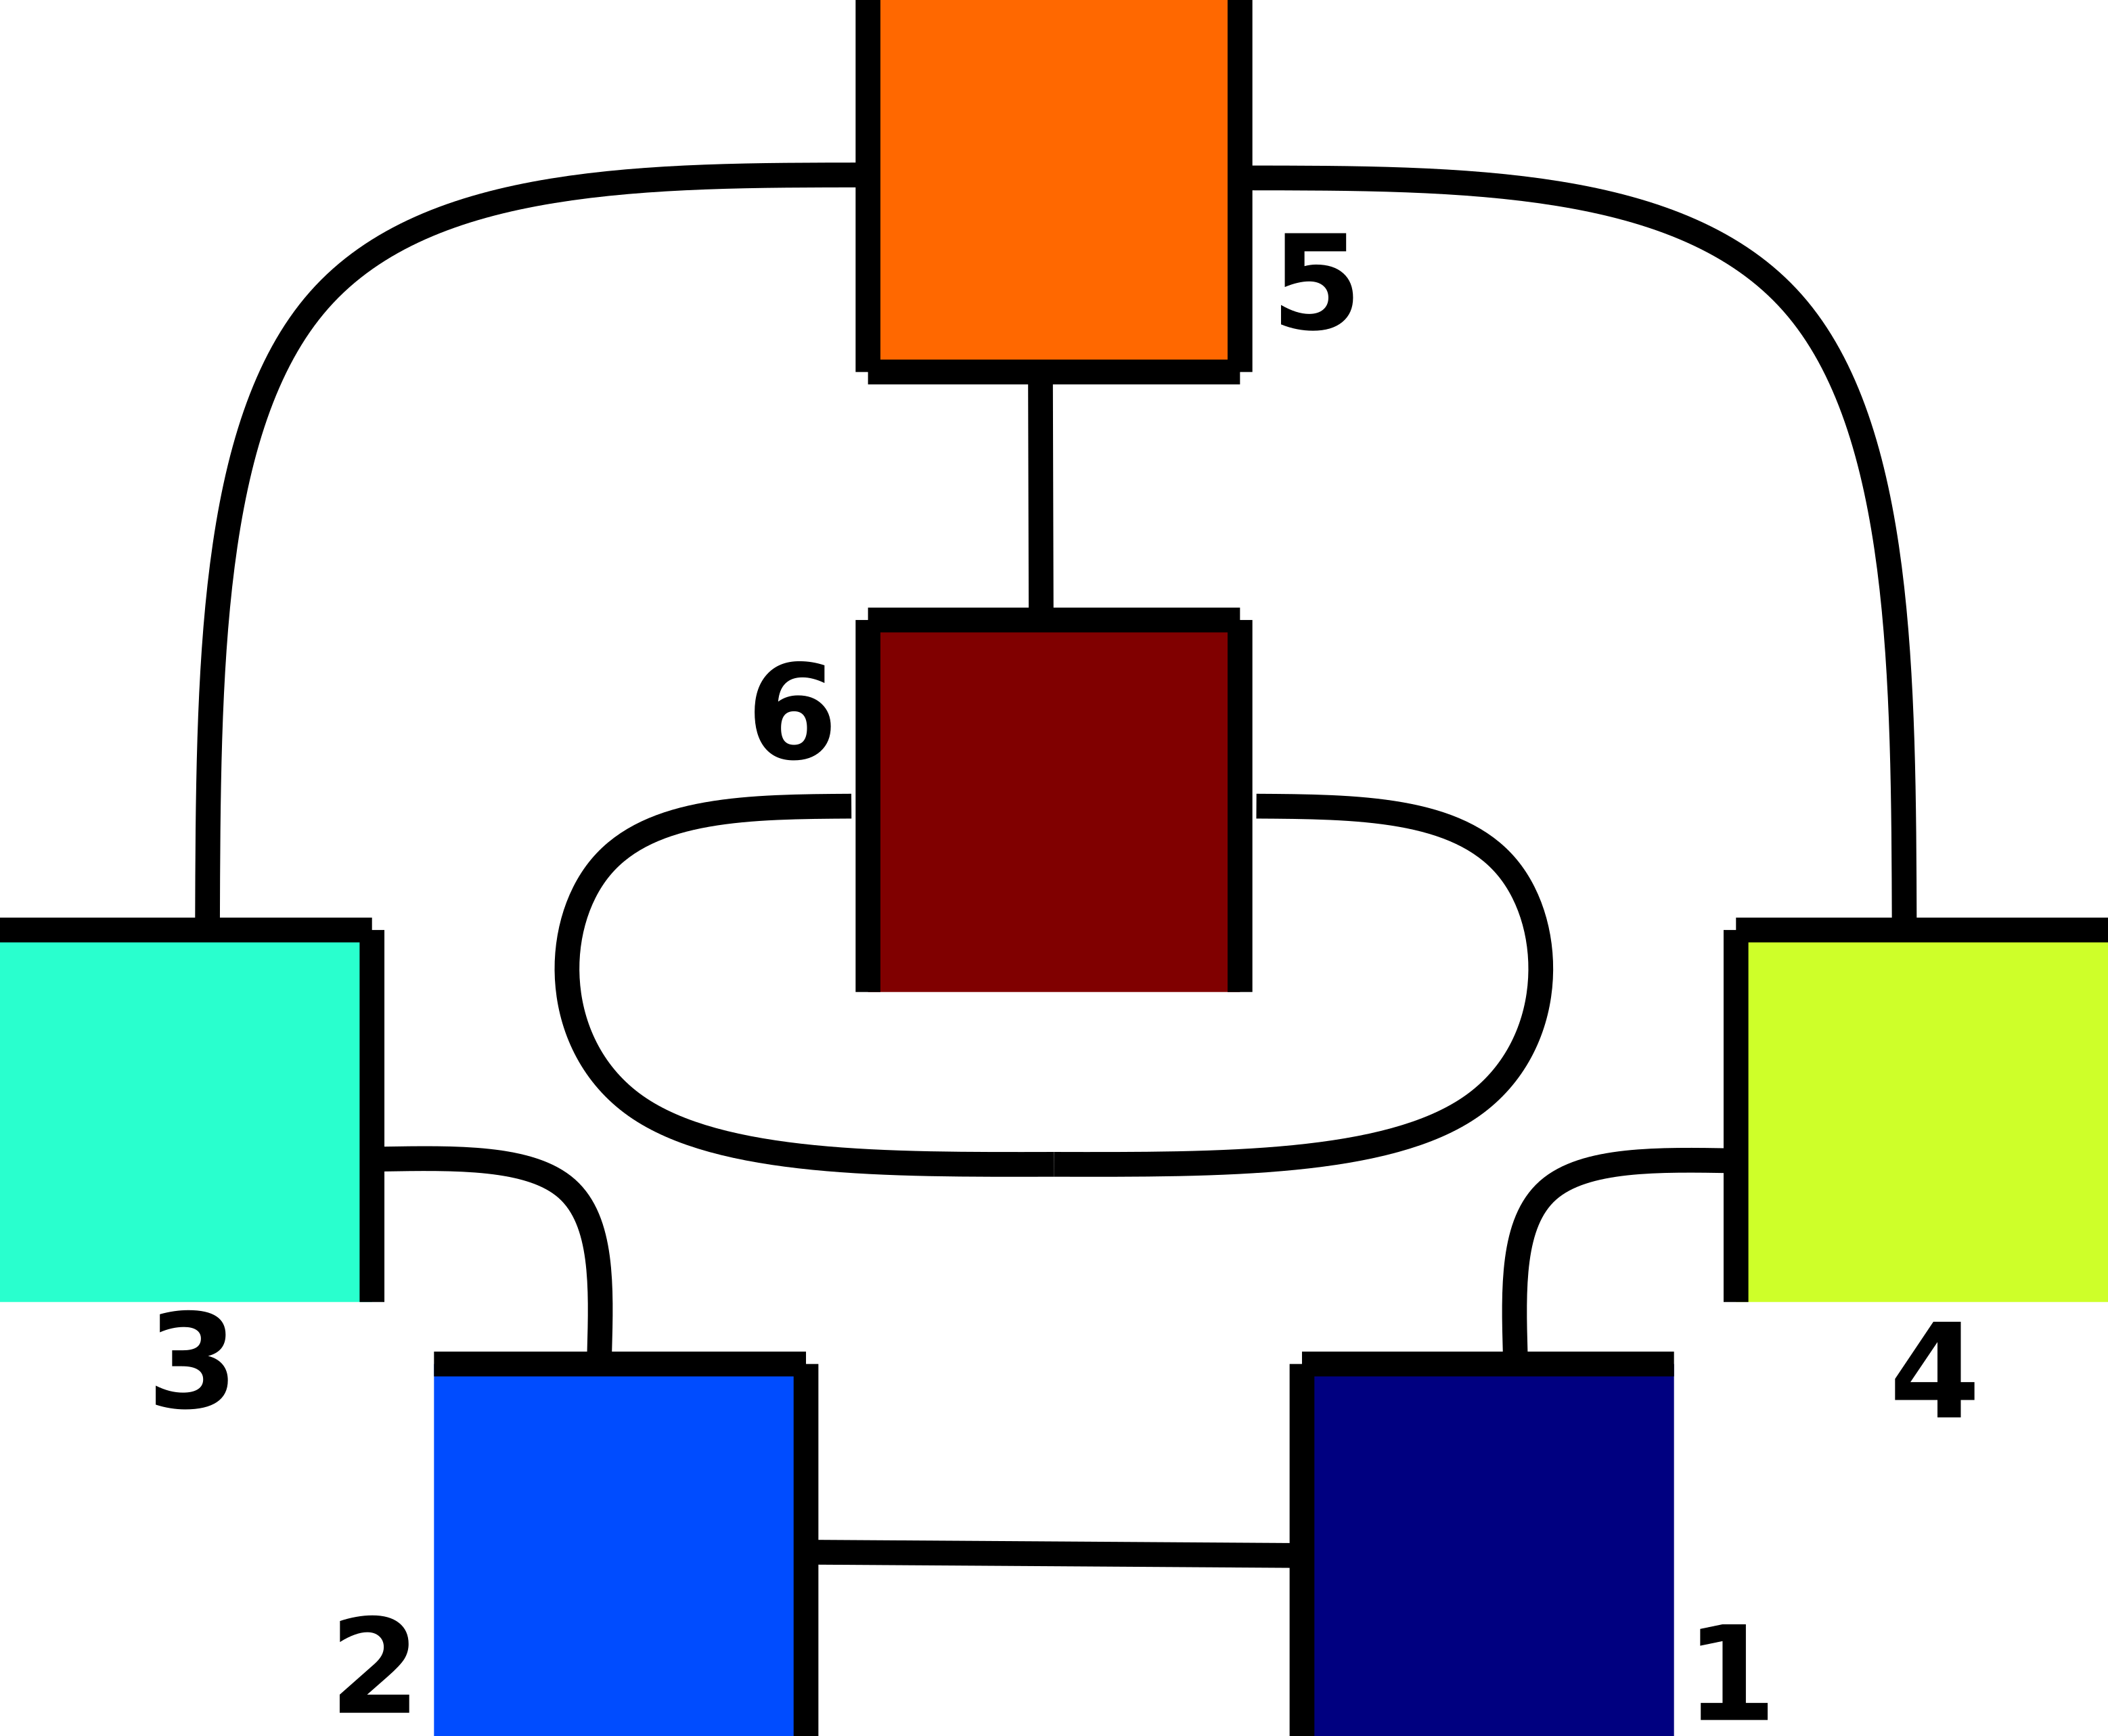
\includegraphics[width=1\textwidth]{schemes/TCV_domains.png}
		\subcaption{Connected zones in the domain decomposition}
		\label{fig:TCV_domains}
	\end{subfigure}
	
	\caption[Example of typical mesh and domain decomposition mapping the real domain to a Cartesian multiple zones domain]{ Example of typical mesh and domain decomposition mapping the real domain (a) to a Cartesian multiple zones domain (b). Each colored zone is isomorphic to a cube, the lines connecting the edges indicate the neighbours mapping. }
	\label{fig:TCVzoneDecomposition}
\end{figure}

\subsection{Curvilinear coordinates}
\label{ssec:MetricCurvilinearCoordinates}

The flux-surface-aligned discretization involves a curved grid in poloidal $\theta$ and toroidal $\varphi$ directions. To map the real geometry to the orthonormal grid on each subdomain, we require a metric transformation. The second chapter of the book by D’haeseleer \emph{et al.}\cite{CurvilinearGrids} describes well the numerical implications of curvilinear grids and serves as the basis of the present implementation. \\

Let $U=[u^\psi, u^\theta, u^\varphi]^T$ be the three parameters that describe every point in the domain $\Omega$ with respect to the curvilinear system of coordinates. On a torus, we can find an invertible transformation $R$ that maps each possible $U\in\Omega$ to a unique point in cartesian coordinates, thus: 

\begin{equation}
	\begin{bmatrix} x \\ y \\ z\end{bmatrix} = \mathbf{R}(u^\psi, u^\theta, u^\varphi)
\end{equation}

If we fix one parameter and allow the two remaining to vary freely, we obtain the so-called coordinate surface. Analogously if we fix two parameters, we obtain the coordinate curve associated to the free parameter and an accommodating choice for the scalar values $u^i$ is the curve length from an arbitrary reference point. At any point $P\in\Omega$, a local basis ${\mathbf{e}_\psi, \mathbf{e}_\theta, \mathbf{e}_\varphi}$ can be defined by the tangents to the respective coordinate curves crossing this point. Consequently, the basis vectors are easily expressed as:

\begin{align}
	\mathbf{e}_\psi =& \pdv{\mathbf{R}}{u^\psi} & \mathbf{e}_\theta =& \pdv{\mathbf{R}}{u^\theta} & \mathbf{e}_\varphi =& \pdv{\mathbf{R}}{u^\varphi}
\end{align}

The parameter choice of $u^i$ can be seen as the curve length and it might or might not be a unit length. The dimension index appears in subscript $\mathbf{e}_i$ to indicate that the basis vectors originate from a $u^i$ located below the fraction line. \\
An alternative basis can be defined from the gradients of the parameters $u^i$ which hence uses a superscript notation:  

\begin{align}
	\mathbf{e}^\psi = & \grad{u^\psi} & \mathbf{e}^\theta = & \grad{u^\theta} & \mathbf{e}^\varphi = & \grad{u^\varphi}
\end{align}

These basis vectors are orthogonal to the respective coordinate surfaces at the point $P$. It can be shown that both basis are reciprocal, thus:
$$ e^i\cdot e_j = \delta^i_j $$
where $\delta^i_j$ is the Kronecker delta. \\
This leads to the introduction of the covariant (linked to subscripts) and contravariant (linked to the superscripts) components of a vector. As it is known from linear algebra, any vector $\mathbf{v}$ can be expressed with respect to an arbitrary basis $\tilde{\mathbf{e}_i}$ as $\mathbf{v}=\tilde{v}_i\tilde{\mathbf{e}}_i$. For the two previously introduced basis, the respective components of $\mathbf{v}$ are given by: 

\begin{align}
	\text{Covariant components: }    & v_i = \mathbf{v}\cdot\mathbf{e}_i & \Rightarrow && \mathbf{v} = v_i\mathbf{e}^i \\
	\text{Contravariant components: }& v^i = \mathbf{v}\cdot\mathbf{e}^i & \Rightarrow && \mathbf{v} = v^i\mathbf{e}_i \\
\end{align}

It is common practice to call the representation of $\mathbf{v}$ using the co-/contravariant components the co-/contravariant vector of $\mathbf{v}$ albeit the co- and contravariant vectors both naturally describe the same vector $\mathbf{v}$. \\
Next, we introduce the metric coefficients $g_{ij} = \mathbf{e}_i\cdot \mathbf{e}_j$ and their reciprocal metric coefficients $g^{ij} = \mathbf{e}^i\cdot \mathbf{e}^j$. If available, they allow for an easy both-way conversion of contravariant to covariant vectors and consequently an easy change of basis. 

\begin{align}
	v_i =& g_{ij}v^j & \mathbf{e}_i =& g_{ij}\mathbf{e}^j \\
	v^i =& g^{ij}v_j & \mathbf{e}^i =& g^{ij}\mathbf{e}_j 
\end{align}

It may be noted that the matrices formed by the indices $i,j\in\{\theta,\psi,\varphi\}$ are each other's inverse matrix. Further details on the curvilinear metric applied to the magnetic configuration are given in App. \ref{app_linearAlgebra}. \\



\section{The staggered mesh}
\label{sec:impl_staggeredMesh}

In order to benefit from the first-order parallel derivative that separates the $A_\parallel$ and $j_\parallel$ from the other plasma fields $\Phi$, $n_e$, and $T_e$ (Eq. \ref{eq:S3X_vorticityEquation_FullElectromagnetic}), these two variables are defined on a toroidally $\varphi$ and poloidally $\theta$ staggered grid. They are calculated at cell edges in the parallel direction and can be directly matched to the fluxes entering and leaving the collocated cells. One of the major benefits is to minimize numerical diffusion and preserve turbulent structures, following findings in FVM simulations for fluid mechanics \cite{meier1999comparison}. In the radial $\psi$ direction, we keep the collocated position as the only parallel gradient in $\psi$ comes from the flutter term, which in nature is much smaller than the equilibrium field. If the mesh were also staggered in $\psi$, we would face strong numerical radial diffusion of parallel fluxes, defying the motivation of a staggered grid for $A_\parallel$ and $j_\parallel$. \newline



\subsection{Description and notation}
The scalar variable $A_\parallel$ is the magnitude of the parallel magnetic vector potential that is a factor of the unit vector $\mathbf{b}$ in direction of the externally induced magnetic field lines. By construction of the domain, $\mathbf{b}$ has only components in $\varphi$ and $\theta$ directions. So far, all physical quantities are calculated on the collocated grid points at the domain cell centers. In the newly introduced equation on $A_\parallel$, the magnetic vector potential appears homogeneous to the potential, pressure and temperature gradients and the additional $A_\parallel$ term in the original equation states that the divergence of $A_\parallel$ accounts for the change in vorticity. Thus, $A_\parallel$ is always one spatial derivative away from the original quantities. As it is common in classical CFD simulation the velocity, $A_\parallel$ is not defined on cell centers but on a staggered grid on the cell edges in $\psi$-direction. Because the magnetic field lines do not evolve in radial direction and only parallel gradients contribute to $A_\parallel$, its grid is only staggered in  poloidal and toroidal directions. To distinguish quantities on both grids, the indexes $[i_\psi, i_\theta - \frac{1}{2},i_\varphi-\frac{1}{2}]$ describe discrete positions on the staggered grid. \\

\begin{figure}[H]
	\centering
	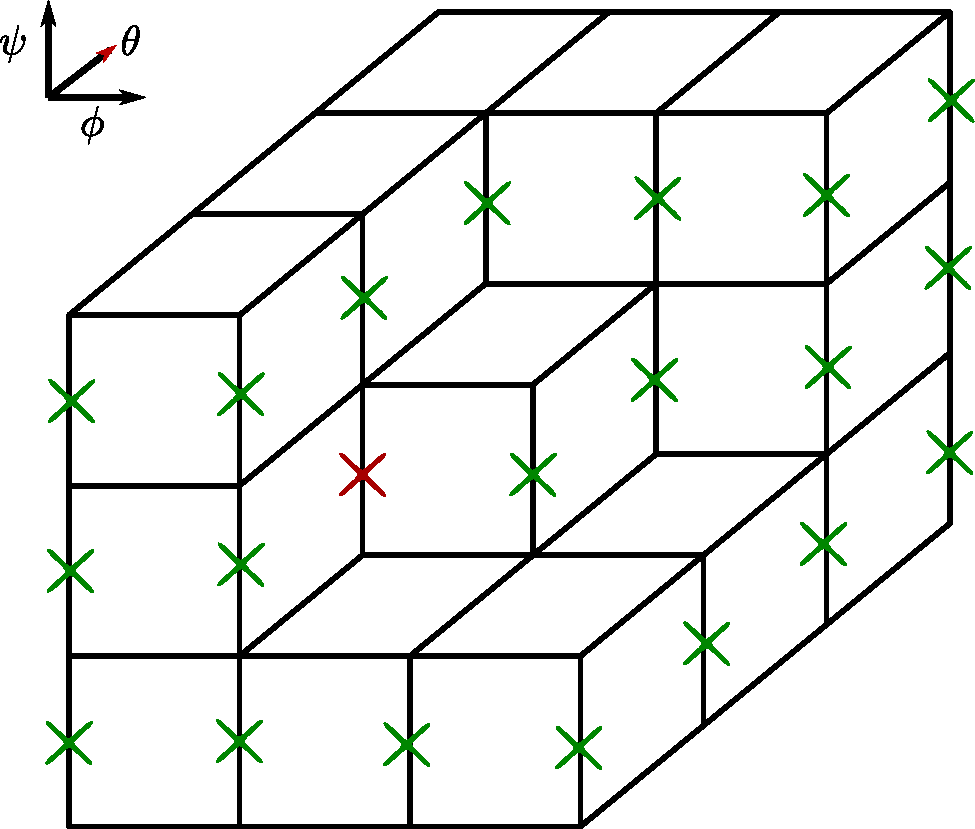
\includegraphics[width=0.4\textwidth]{schemes/StaggeredGrid.pdf}
	\caption[General view of the staggered grid points marked as crosses on top of the collocated cells]{General view of the staggered grid points marked as crosses on top of the collocated cells. The red cross at the position $[i_\psi, i_\theta - \frac{1}{2}, i_\varphi-\frac{1}{2}]$ corresponds to the central cell with index $[i_\psi, i_\theta, i_\varphi]$}
	\label{fig:StaggeredGridOverview}
\end{figure}

In the following work, quantities evaluated at staggered grid points are indicated either by the superscript $stg$ or by a $-\frac{1}{2}$ shift in the index. This means that following notations are equivalent: 
\begin{align*}
	X^{stg}_{[i_\psi,i_\theta,i_\varphi]} &= X_{[i_\psi,i_\theta-\frac{1}{2},i_\varphi-\frac{1}{2}]} &\text{or}&& X^{stg}_{[i_\psi,i_\theta+1,i_\varphi]} &= X_{[i_\psi,i_\theta+\frac{1}{2},i_\varphi-\frac{1}{2}]}
\end{align*}



\subsection{Boundary cells}

Staggered quantities require a different treatment at the domain boundary. On the collocated mesh, cells are located either entirely in the plasma or in the physical wall. Staggered quantities in the boundary layer are thus always half a cell width away from the wall and boundary conditions are enforced accordingly. For the magnetic vector potential this holds for walls in $\psi$ direction but in $\varphi$ and $\theta$ directions, the staggered grid points are on the tokamak wall for the boundary cells with lowest index and one cell width away at the highest index. For consistency, accuracy and symmetry purposes, the staggered solvable domain shall be either extended by one row of cells at the upper index to include the wall in the solution or or reduced by one row at the lower end. In both cases, the number of collocated and staggered grid points do not match anymore and inhibit all eventual symmetry properties of the matrix in the dual-grid system. $A_\parallel$ requires Dirichlet boundary conditions with the value 0 everywhere, thus the solution on the wall is already known and is not needed in the system. The parallel current $j_\parallel$ is fixed by the sheath current perpendicular to the wall, but is still needed for the parallel component tangential to the sheath. In Fig. \ref{fig:StaggeredGridBC}, the position of the staggered fields $A_\parallel$ and $j_\parallel$ along the wall is shown.

\begin{figure}[H]
	\centering
	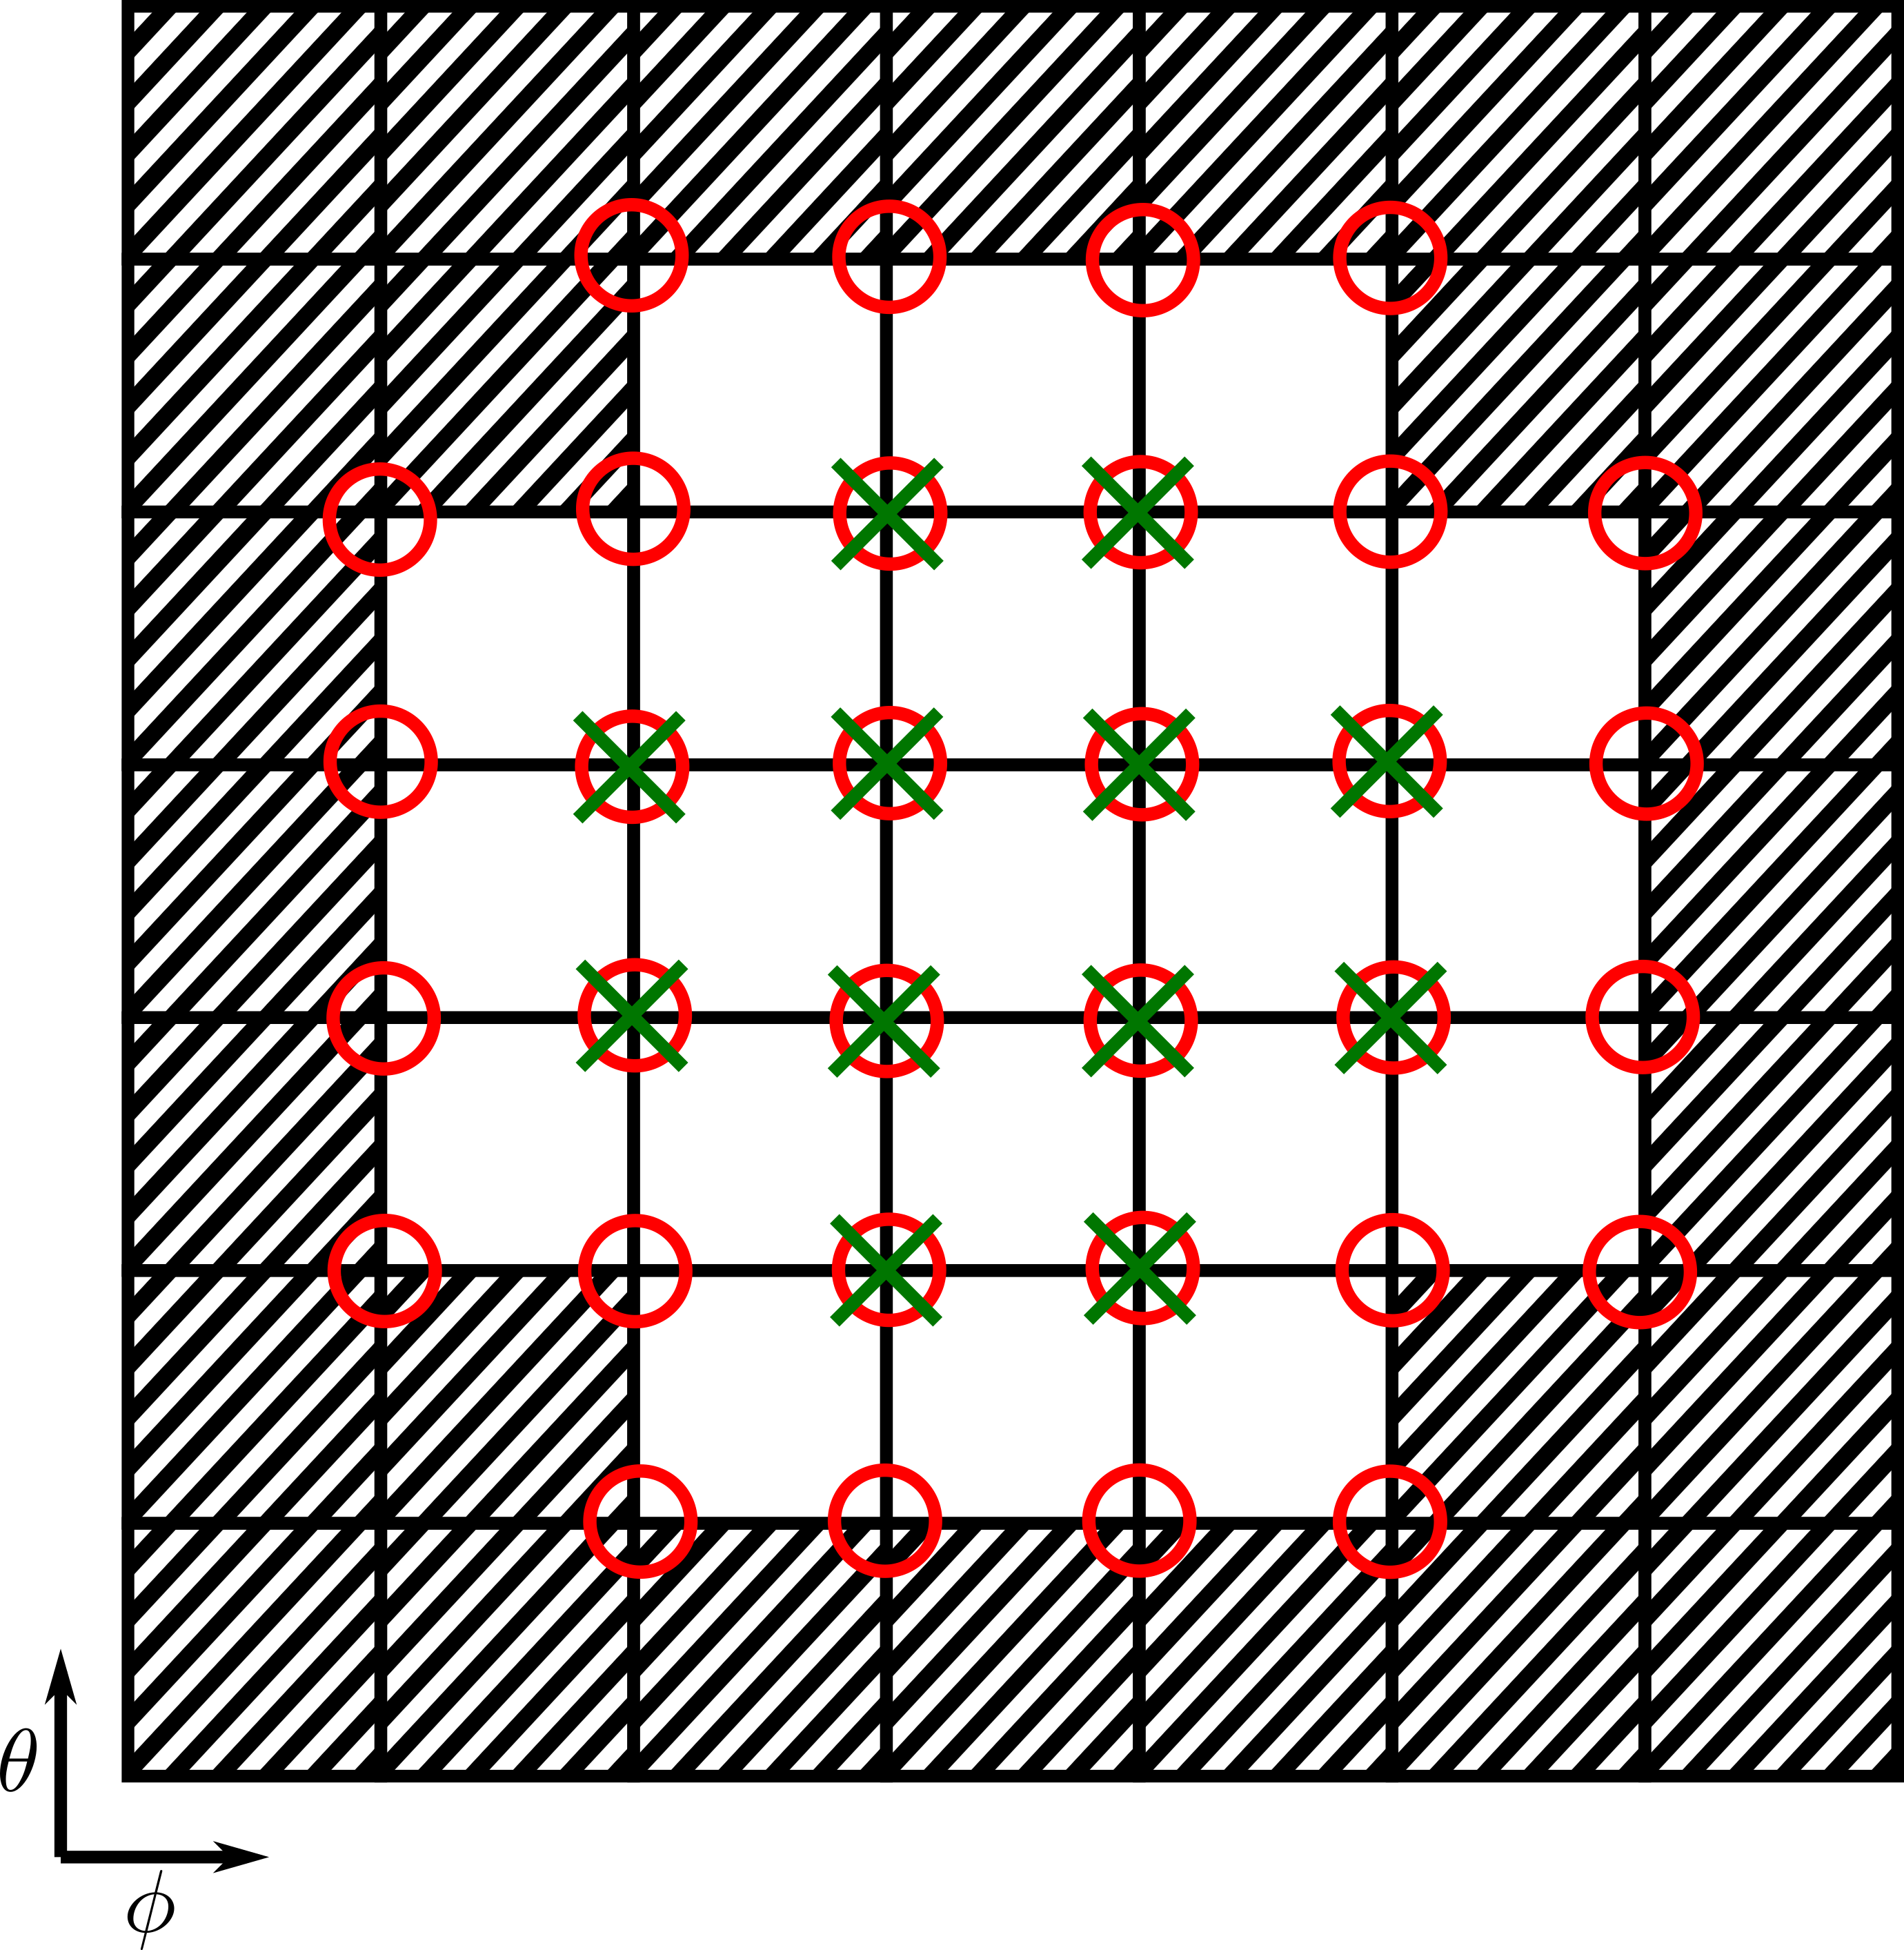
\includegraphics[width=0.6\textwidth]{schemes/staggeredGridBoundary.png}
	\caption[General view of the staggered grid points in the $\theta-\varphi$ plane]{General view of the staggered grid points in the $\theta-\varphi$ plane. The field $A_\parallel$ is defined at the green crosses and $j_\parallel$ at the red circles. Crossed cells are boundary cells where the mask is $\chi = 1$. }
	\label{fig:StaggeredGridBC}
\end{figure}

To ensure a correct implementation of the system and the stencils that appear in it, a new mask describes which cells contain staggered grid points in the solvable domain. It is defined from the original collocated wall mask $\chi$ as:

\begin{align}
	\label{eq:def_chi_staggered}
	\chi^{A_\parallel}_{[i_\psi,i_\theta, i_\varphi]} &= 1 - 
	(1 - \chi_{[i_\psi,i_\theta  ,i_\varphi  ]})
	(1 - \chi_{[i_\psi,i_\theta-1,i_\varphi  ]})
	(1 - \chi_{[i_\psi,i_\theta  ,i_\varphi-1]})
	(1 - \chi_{[i_\psi,i_\theta-1,i_\varphi-1]}) \\
	\chi^{j_\parallel}_{[i_\psi,i_\theta, i_\varphi]} &= 
	\chi_{[i_\psi,i_\theta  ,i_\varphi  ]}
	\chi_{[i_\psi,i_\theta-1,i_\varphi  ]}
	\chi_{[i_\psi,i_\theta  ,i_\varphi-1]}
	\chi_{[i_\psi,i_\theta-1,i_\varphi-1]}
\end{align}

The value of $\chi^{A_\parallel}$ is therefore 1 if the staggered cell with index $[i_\psi,i_\varphi,i_\theta]$ overlaps with the wall and is 0 inside the solvable domain. Conversely, the mask $\chi^{j_\parallel}$ is 0 unless the entire cell lies in the wall. 


Let us discuss a bit further sheath boundary conditions for staggered fields, where $A_\parallel$ and $j_\parallel$ lie on the domain boundary. For collocated fields, we impose sheath fluxes from the Bohm-Chodura model (see Sec. \ref{sec:S3X_boundaryConditions}) on the first cell in the simulation domain. For the magnetic potential $A_\parallel$, the 0-Dirichlet condition is imposed in the concerned cell. For the parallel current $j_\parallel$, we add the sheath current $j_{\text{wall}}$ to any parallel currents tangential to the wall. Indeed, if the sheath boundary is in the $\theta$ direction, the $\varphi$ component of the parallel current remains unaffected and needs to be solved. 



\subsection{Staggered discrete operators}
As the parallel current $j_\parallel$ and the magnetic vector potential $A_\parallel$ are defined on a staggered grid, new stencil operators are needed to be compatible with the electric potential $\Phi$ defined on the collocated grid at the cell centers. 



\subsubsection{Parallel gradient}

To calculate the parallel current in Ohm's law, we require the parallel gradients of potential, density and electron temperature. The three fields are defined on the collocated grid, and the result of the operator shall lie on the staggered grid. 

\begin{equation}
	\left[\grad_{\parallel}X\right]^{stg}_{[i_\psi,i_\theta, i_\varphi]}
\end{equation}

Wave structure travel along the parallel direction, dominated by the equilibrium field $\mathbf{b}_{eq}$ in $\theta$ and $\varphi$-directions. Because of the high anisotropy given $B_{eq,p} \ll B_{eq,\varphi}$, this operator is prone to numerical dissipation if not properly implemented. Both directions are calculated in a common step

\begin{align}
	\left[\textbf{b}_{eq}\cdot\grad X \right]^{stg}_{[i_\psi,i_\theta, i_\varphi]} = \frac{1}{2}&\left(
	\left(+b^\theta_{stg} + b^\varphi_{stg}\right)X_{[i_\psi,i_\theta, i_\varphi]} + 
	\left(-b^\theta_{stg} + b^\varphi_{stg}\right)X_{[i_\psi,i_\theta-1, i_\varphi]} \right. \nonumber\\  &+ \left. 
	\left(+b^\theta_{stg} - b^\varphi_{stg}\right)X_{[i_\psi,i_\theta, i_\varphi-1]} + 
	\left(-b^\theta_{stg} - b^\varphi_{stg}\right)X_{[i_\psi,i_\theta-1, i_\varphi-1]}\right)
	\label{eq:Impl_GradParaStencil_FS}
\end{align}

This discrete operator involves four neighbors, as shown in Fig. \ref{fig:Impl_GradPara_ThetaPhi}. It is appreciated in the finite elements community for anisotropic wave propagation\cite{yee1966numerical,rubio2014finite, hasegawa2012staggered} for its good numerical properties and is used in the anisotropic heat diffusion problem in magnetized plasmas by Günter et al\cite{gunter2005}.


\begin{figure}[H]
	\centering
	\begin{subfigure}[t]{0.40\textwidth}
		\centering
		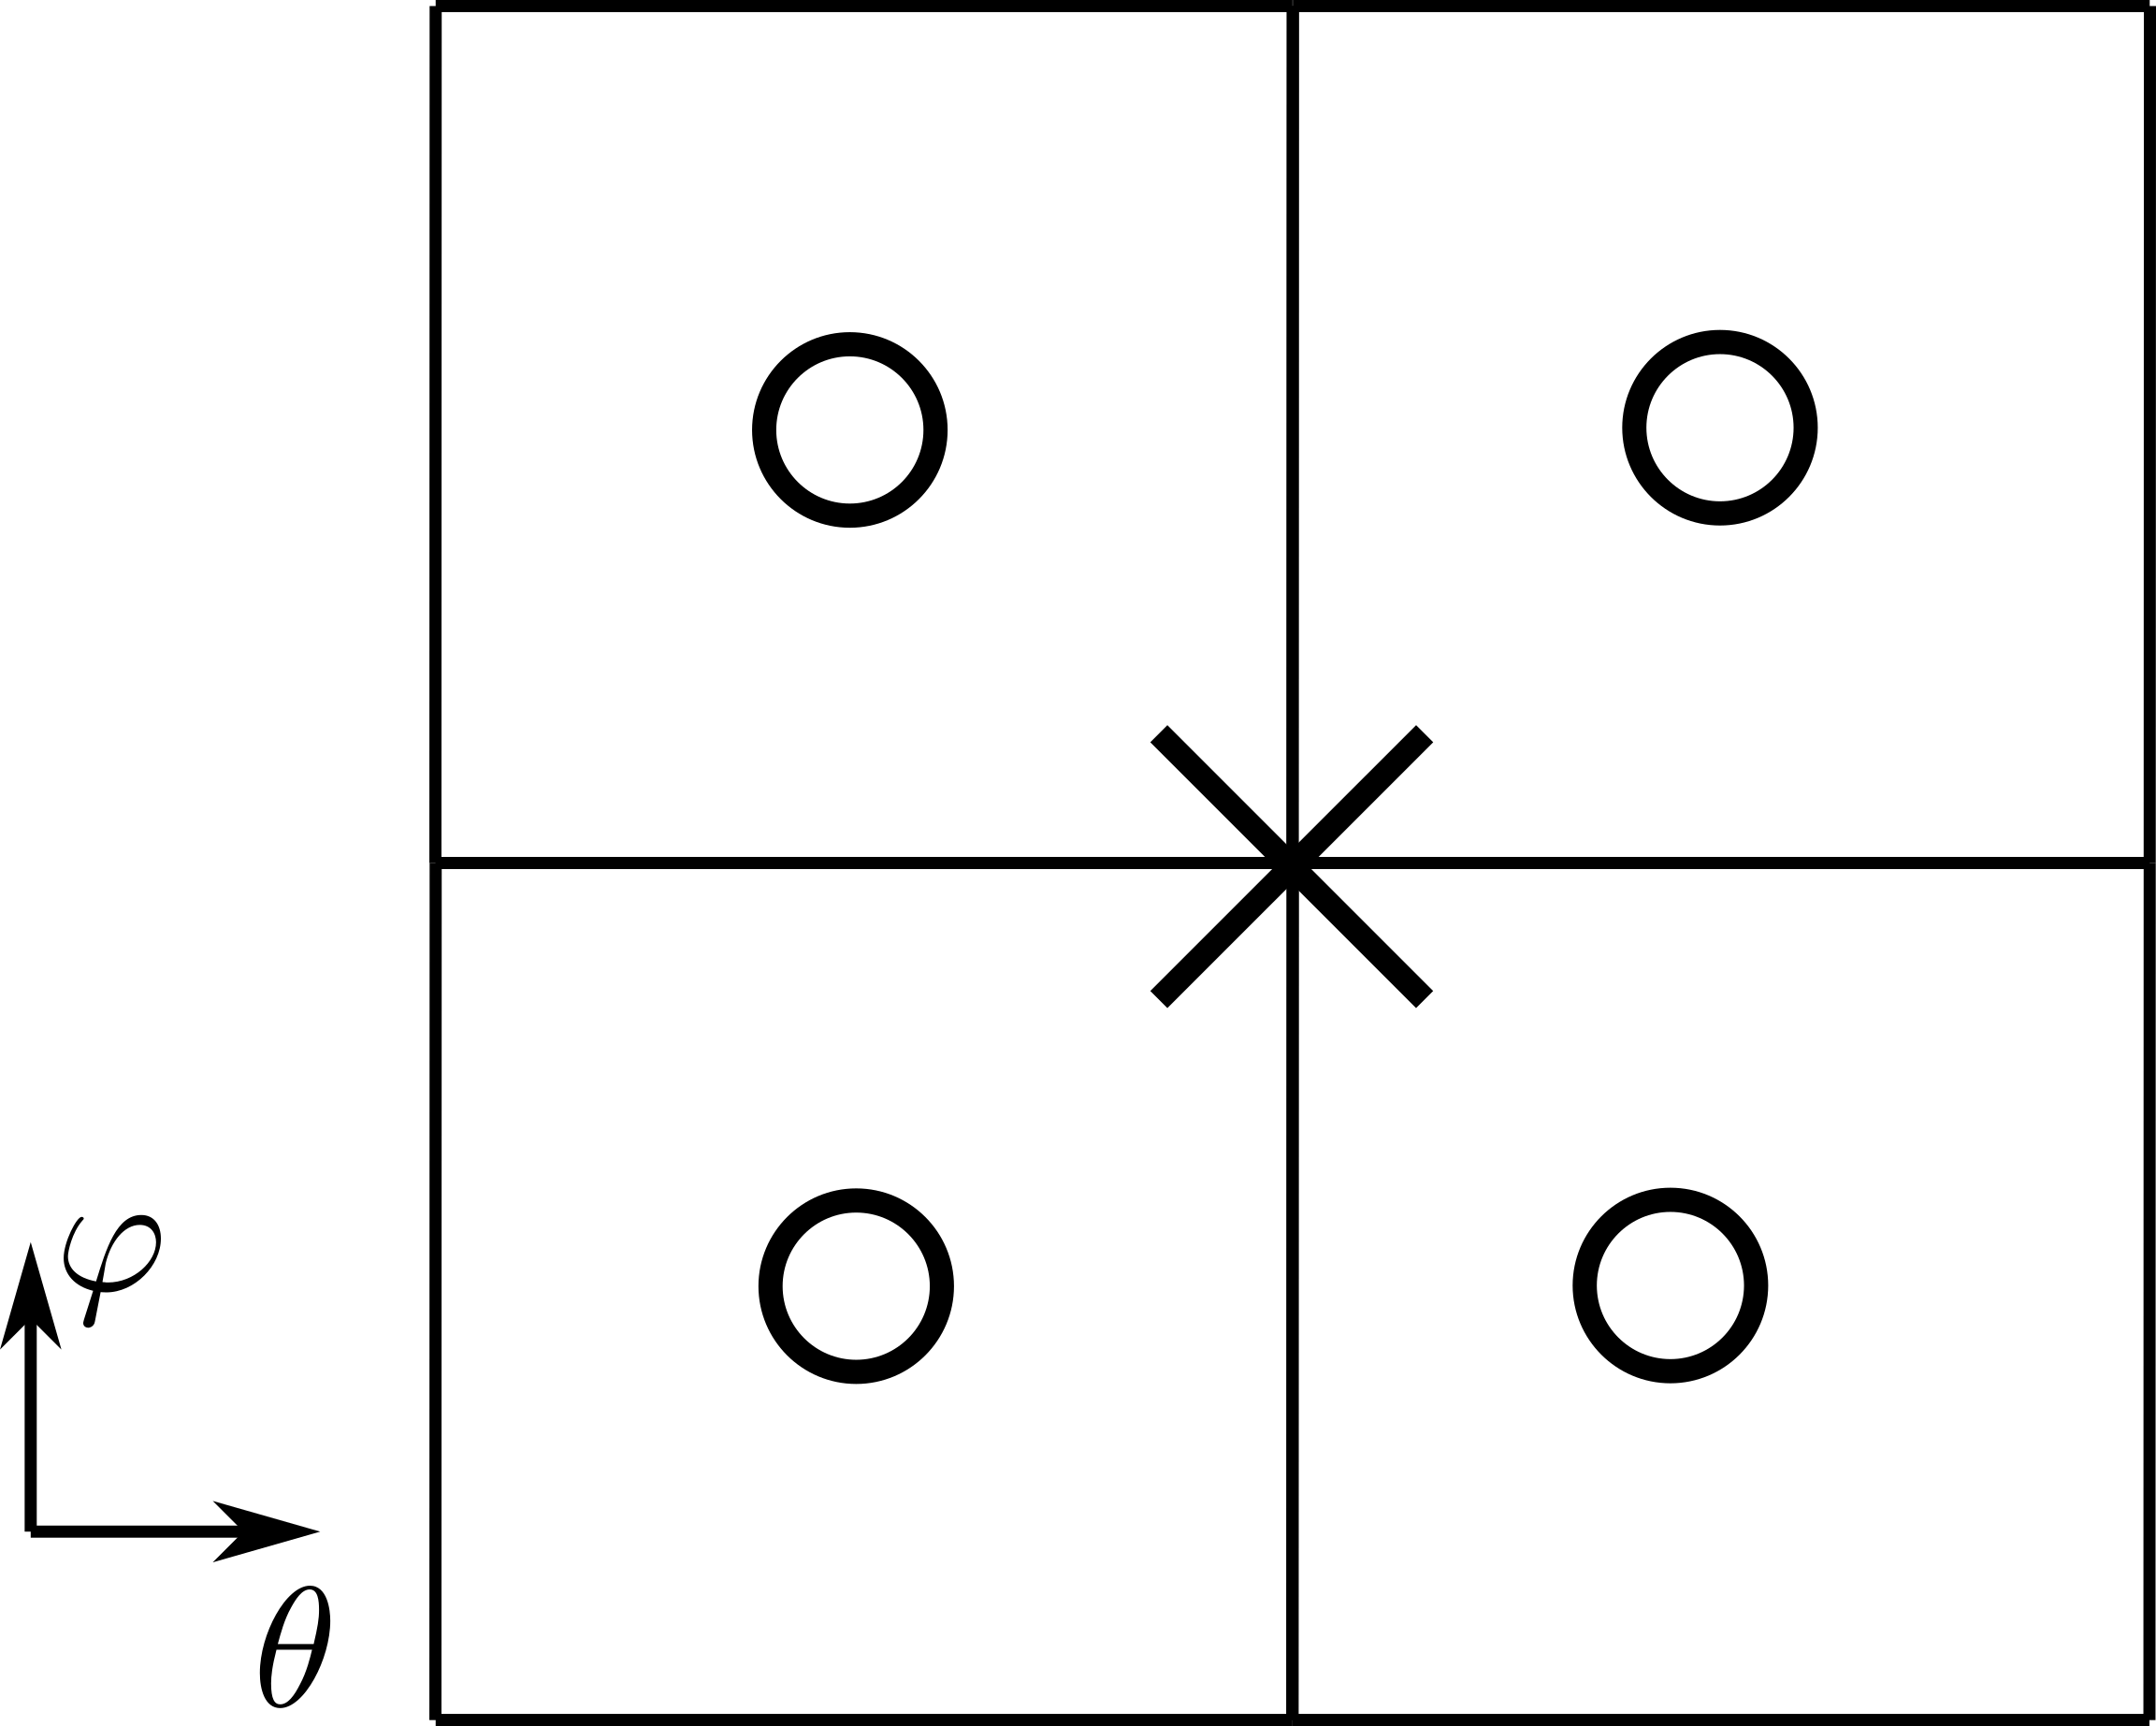
\includegraphics[height=40mm]{schemes/GradientStencil_ThetaPhi.png}
		\subcaption{Gradient along the equilibrium field}
		\label{fig:Impl_GradPara_ThetaPhi}
	\end{subfigure}
	\begin{subfigure}[t]{0.55\textwidth}
		\centering
		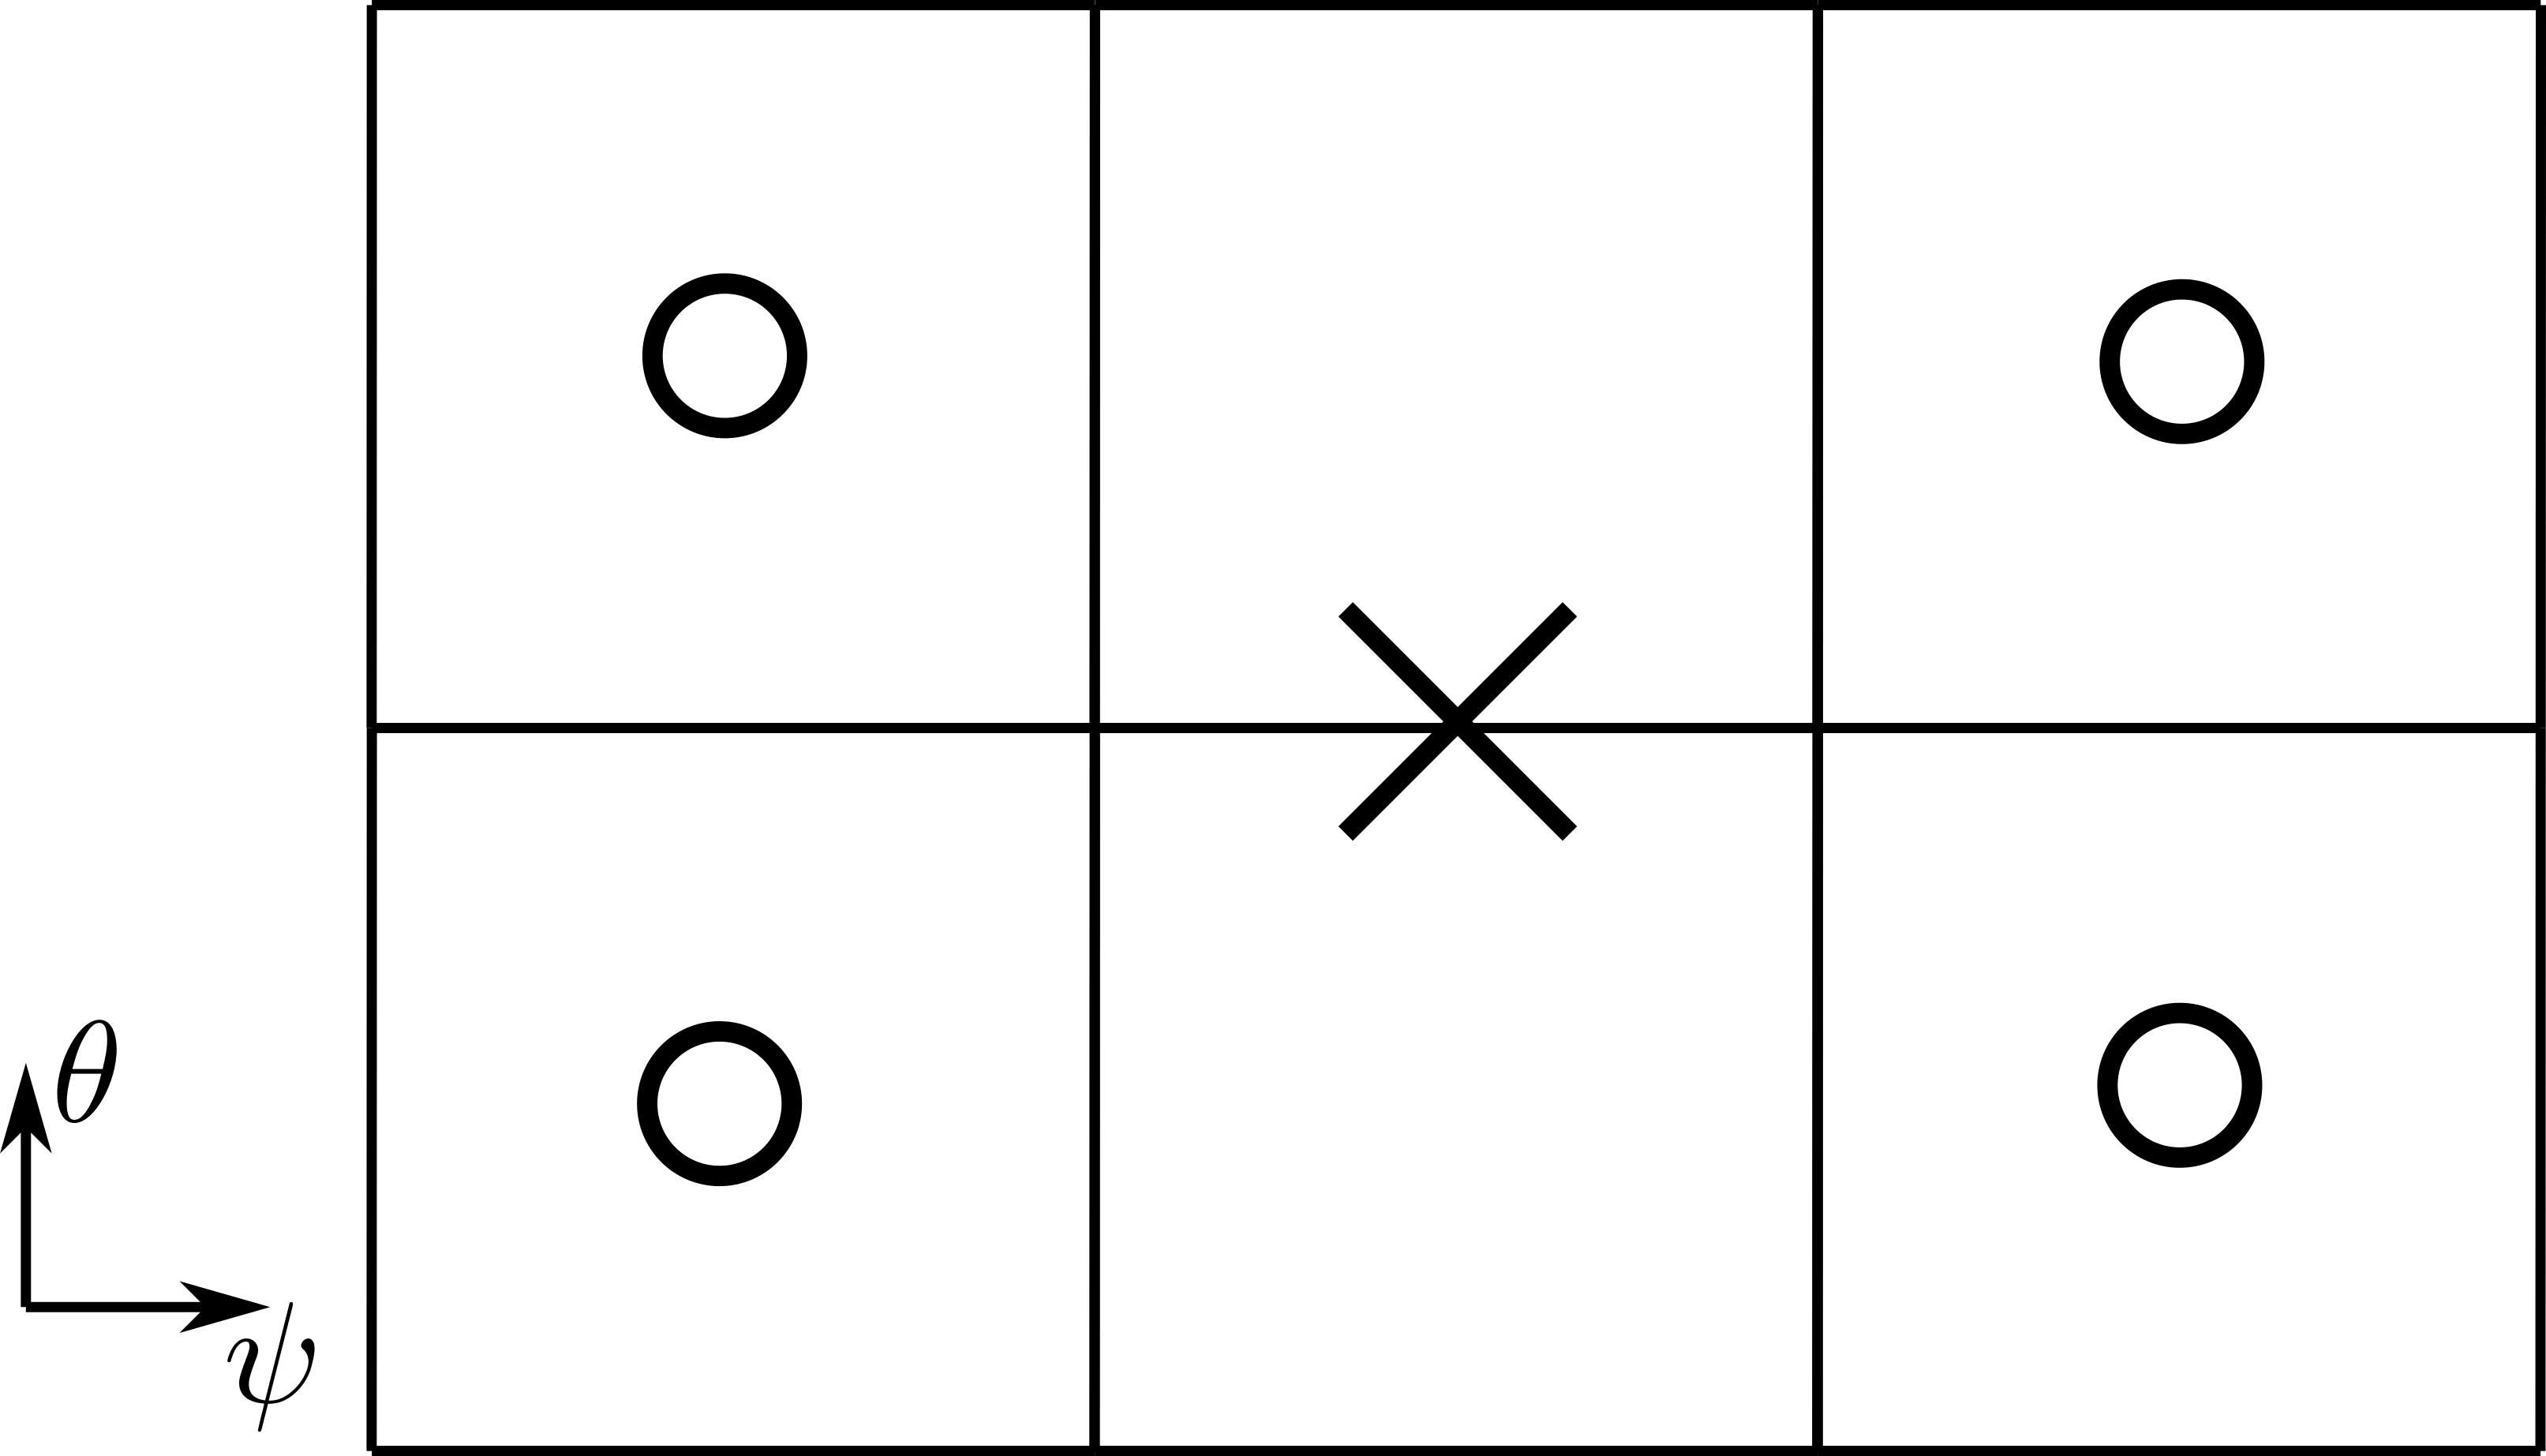
\includegraphics[height=40mm]{schemes/GradientStencil_PsiTheta.png}
		\subcaption{Gradient in radial direction}
		\label{fig:Impl_GradPara_PsiTheta}
	\end{subfigure}
	\caption[Neighbors involved to calculated staggered parallel gradients]{Neighbors involved to calculated staggered parallel gradients.}
	\label{fig:Impl_GradPara}
\end{figure}

The gradient in radial direction, that comes from the magnetic flutter, is treated in a separate step. Because of the staggered grid configuration, that does not apply to the radial direction, the gradient requires 8 neighbors, of which four are shown in Fig. \ref{fig:Impl_GradPara_PsiTheta}, the other four being out of plane in the next poloidal plane.


\begin{align}
	\left[\tilde{\textbf{b}}\cdot\grad X \right]^{stg}_{[i_\psi,i_\theta, i_\varphi]} = \frac{1}{4}b^\psi_{stg}
	&\left( 
	  X_{[i_\psi+1,i_\theta, i_\varphi]} - X_{[i_\psi-1,i_\theta, i_\varphi]} 
	+  X_{[i_\psi+1,i_\theta, i_\varphi-1]} - X_{[i_\psi-1,i_\theta, i_\varphi-1]} \right. \nonumber \\ 
	&+ \left. X_{[i_\psi+1,i_\theta-1, i_\varphi]} - X_{[i_\psi-1,i_\theta-1, i_\varphi]} 
	+  X_{[i_\psi+1,i_\theta-1, i_\varphi-1]} - X_{[i_\psi-1,i_\theta-1, i_\varphi-1]}\right)
	\label{eq:Impl_GradParaStencil_flutter}
\end{align}



The poloidal and toroidal components of the magnetic flutuations are solved together with the equilibrium part in Eq. \ref{eq:Impl_GradParaStencil_FS}.


\subsubsection{Parallel divergence}

The divergence of $j_\parallel$ needs to be calculated at the collocated grid in the vorticity equation. It is the counterpart to the gradient operator above, and calculates the divergence on the collocated grid based on staggered fields. 

\begin{equation}
	\left[\grad\cdot X^{stg}\mathbf{b}\right]_{[i_\psi,i_\theta, i_\varphi]}
\end{equation}

In Eq. \ref{eq:MetricDivergenceParallel}, the divergence of a parallel vector field has been introduced. We consider a collocated cell as in Fig. \ref{fig:StaggeredGridOverview}. The divergence is then the sum of all in- and outgoing fluxes $\pdv{\left(J X b^i\right)}{u^i}$ across the six cell faces. 

\begin{equation}
	\label{eq:NumericalStaggeredDivergenceStencil}
	\left[\grad\cdot X^{stg}\mathbf{b}\right]_{[i_\psi,i_\theta, i_\varphi]} = \frac{1}{J_{[i_\psi,i_\theta, i_\varphi]}} \left(F_{[i_\psi,i_\theta, i_\varphi]}^{X,\psi}-F_{[i_\psi+1,i_\theta, i_\varphi]}^{X,\psi} + F_{[i_\psi,i_\theta, i_\varphi]}^{X,\theta}-F_{[i_\psi,i_\theta+1, i_\varphi]}^{X,\theta}+F_{[i_\psi,i_\theta, i_\varphi]}^{X,\varphi}-F_{[i_\psi,i_\theta, i_\varphi+1]}^{X,\varphi}\right)
\end{equation}

We want calculate these fluxes from the flux $F^{X,i} = JXb^i$ of the staggered field $X^{stg}$. As centered cell faces do not overlap with the staggered grid, we need to take the interpolate the fluxes calculated at the staggered mesh onto the cell face. For the equilibrium direction it involves two neighbors per flux (see Fig. \ref{fig:Impl_DivPara_ThetaPhi}). As an example, here are the fluxes written out for the incoming poloidal flux:

\begin{align*}
	F_{[i_\psi,i_\theta, i_\varphi]}^{X,\theta} &= \frac{1}{2}\left(F_{[i_\psi,i_\theta-\frac{1}{2}, i_\varphi-\frac{1}{2}]}^{X,\theta} + F_{[i_\psi,i_\theta-\frac{1}{2}, i_\varphi+\frac{1}{2}]}^{X,\theta} \right)
\end{align*}

In the radial direction, we need, again, the fluxes at eight neighboring staggered locations (see Fig. \ref{fig:Impl_DivPara_PsiTheta}) to calculate a flux on a single cell face. 

\begin{align*}
	F_{[i_\psi,i_\theta, i_\varphi]}^{X,\psi} = \frac{1}{8}&\left(
	F_{[i_\psi,i_\theta-\frac{1}{2}, i_\varphi-\frac{1}{2}]}^{X,\psi} + 
	F_{[i_\psi,i_\theta-\frac{1}{2}, i_\varphi+\frac{1}{2}]}^{X,\psi} +
	F_{[i_\psi,i_\theta+\frac{1}{2}, i_\varphi-\frac{1}{2}]}^{X,\psi} + 
	F_{[i_\psi,i_\theta+\frac{1}{2}, i_\varphi+\frac{1}{2}]}^{X,\psi} 
	\right. \nonumber \\ &+\left.
	F_{[i_\psi-1,i_\theta-\frac{1}{2}, i_\varphi-\frac{1}{2}]}^{X,\psi} + 
	F_{[i_\psi-1,i_\theta-\frac{1}{2}, i_\varphi+\frac{1}{2}]}^{X,\psi} + 
	F_{[i_\psi-1,i_\theta+\frac{1}{2}, i_\varphi-\frac{1}{2}]}^{X,\psi} + 
	F_{[i_\psi-1,i_\theta+\frac{1}{2}, i_\varphi+\frac{1}{2}]}^{X,\psi} 	
	\right)
\end{align*}

\begin{figure}[H]
	\centering
	\begin{subfigure}[t]{0.48\textwidth}
		\centering
		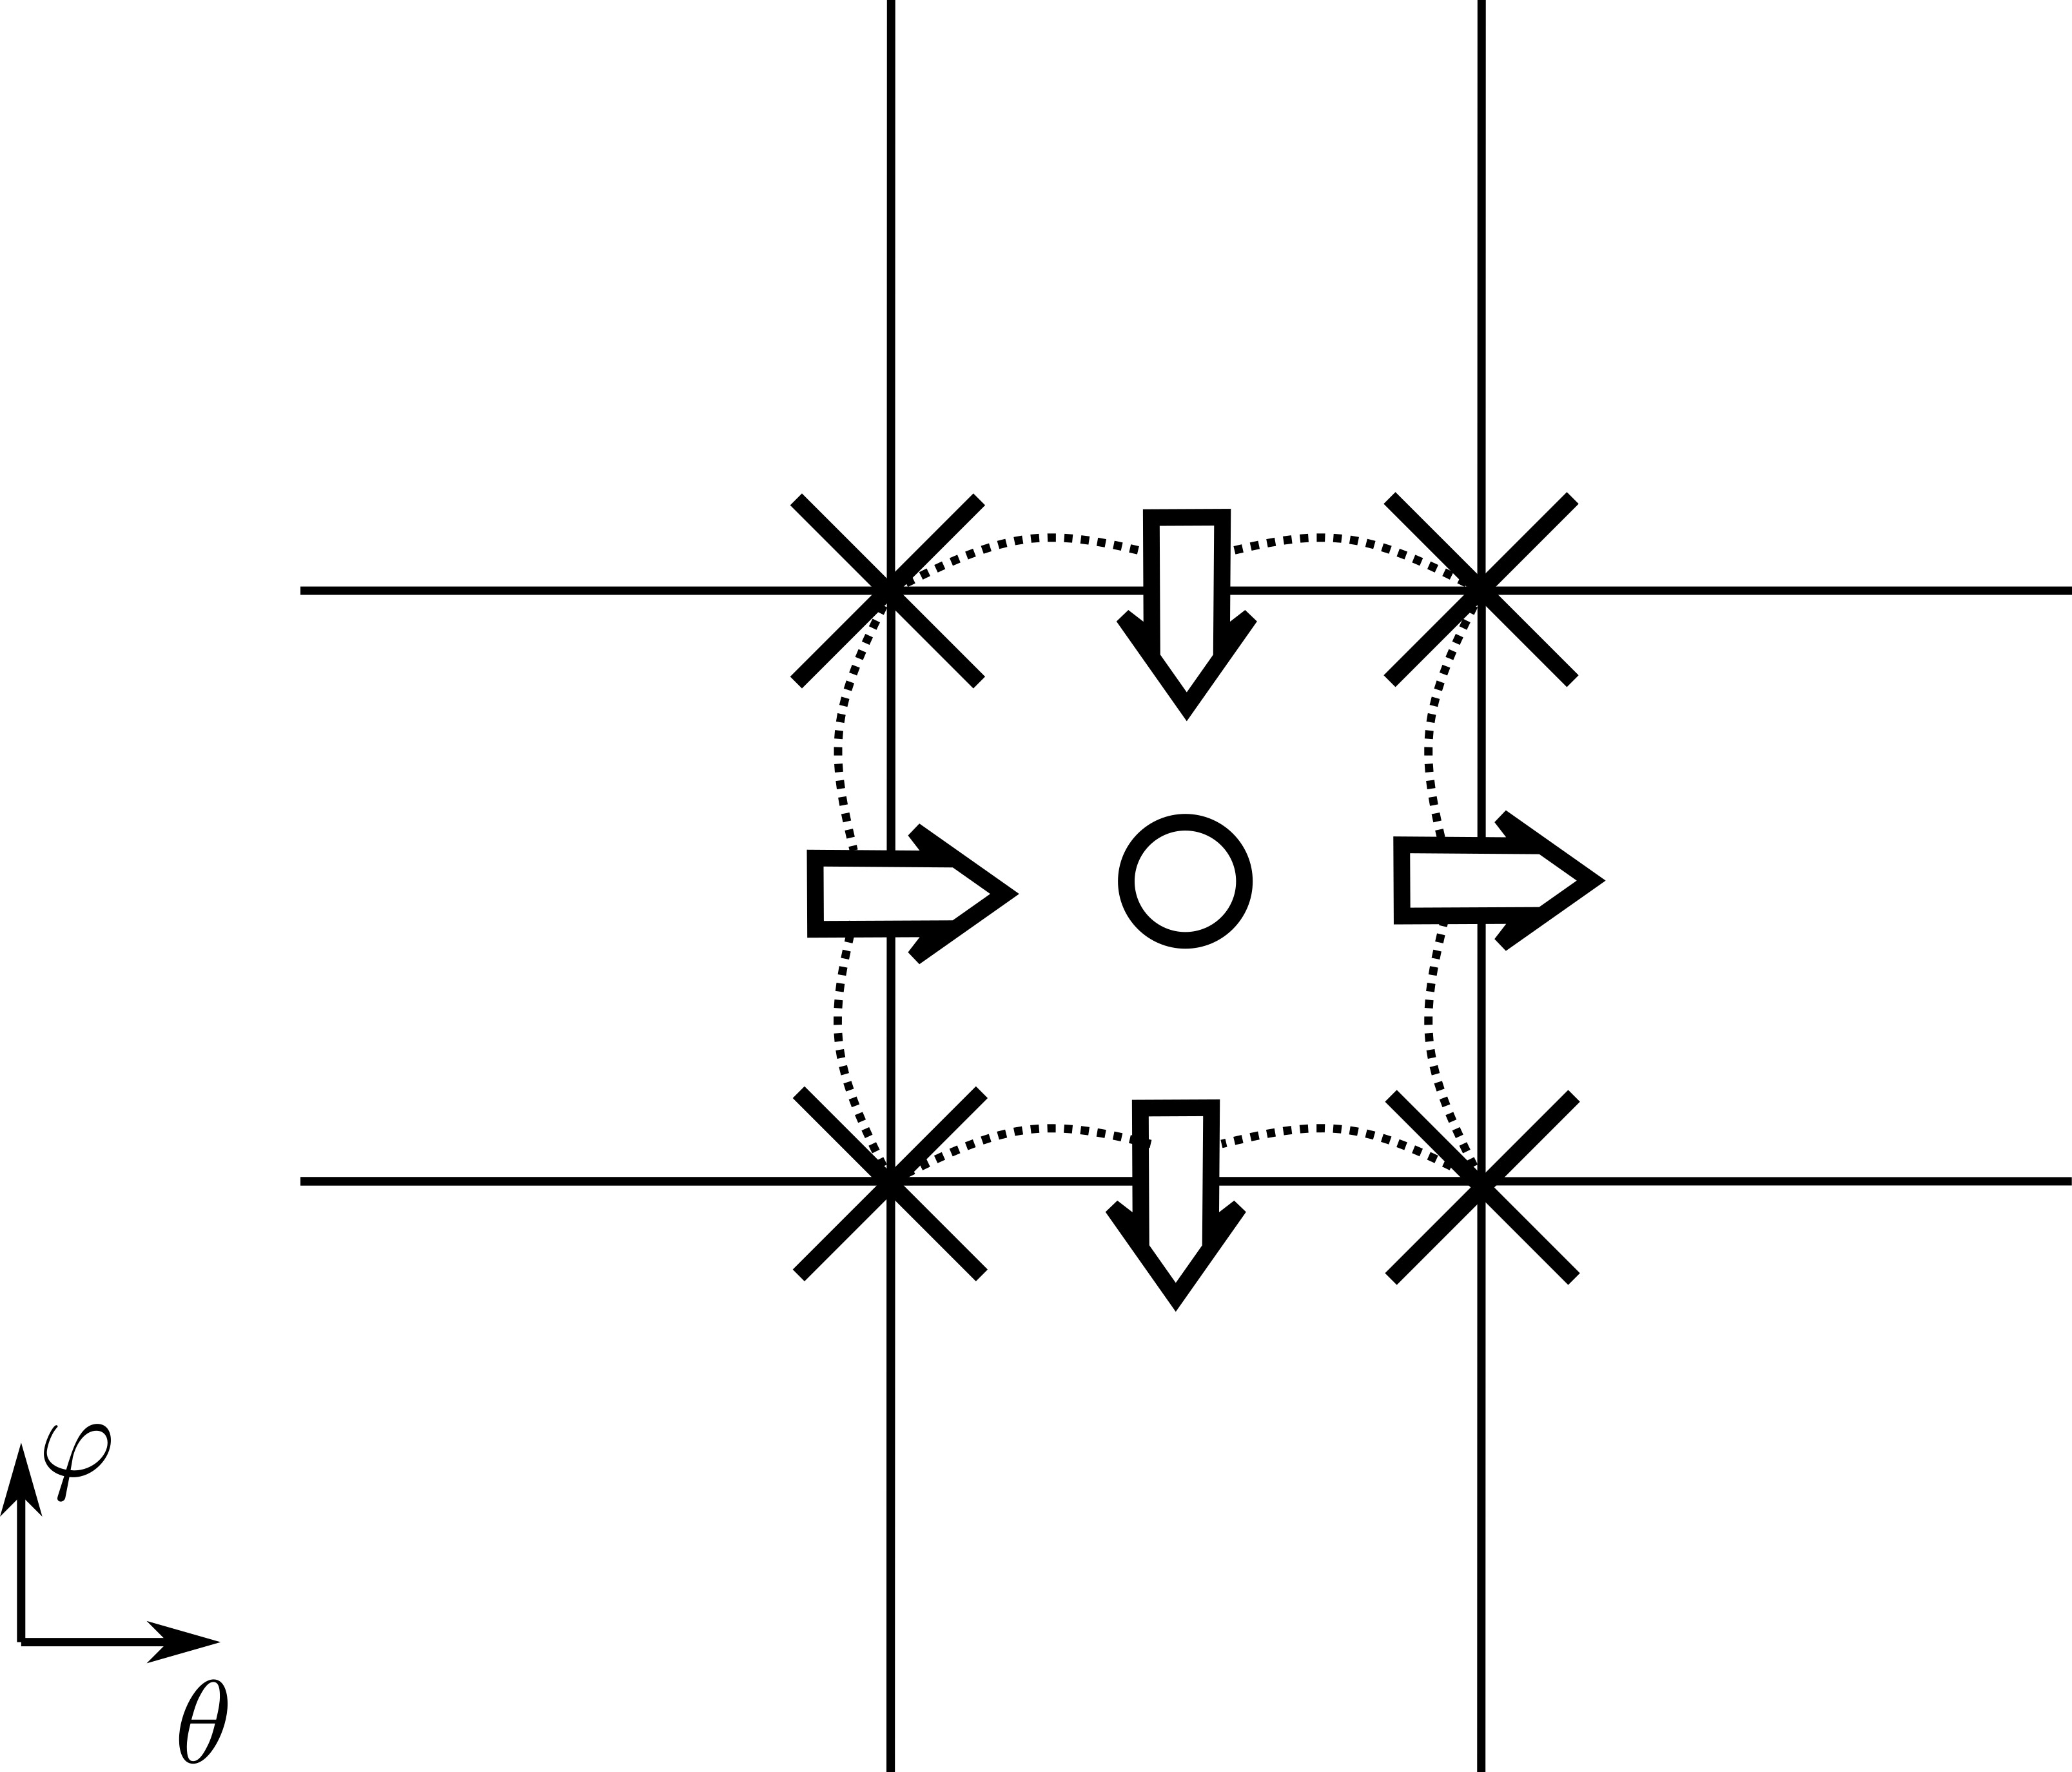
\includegraphics[height=60mm]{schemes/DivStencil_ThetaPhi.jpg}
		\subcaption{Divergence along the equilibrium field}
		\label{fig:Impl_DivPara_ThetaPhi}
	\end{subfigure}
	\begin{subfigure}[t]{0.48\textwidth}
		\centering
		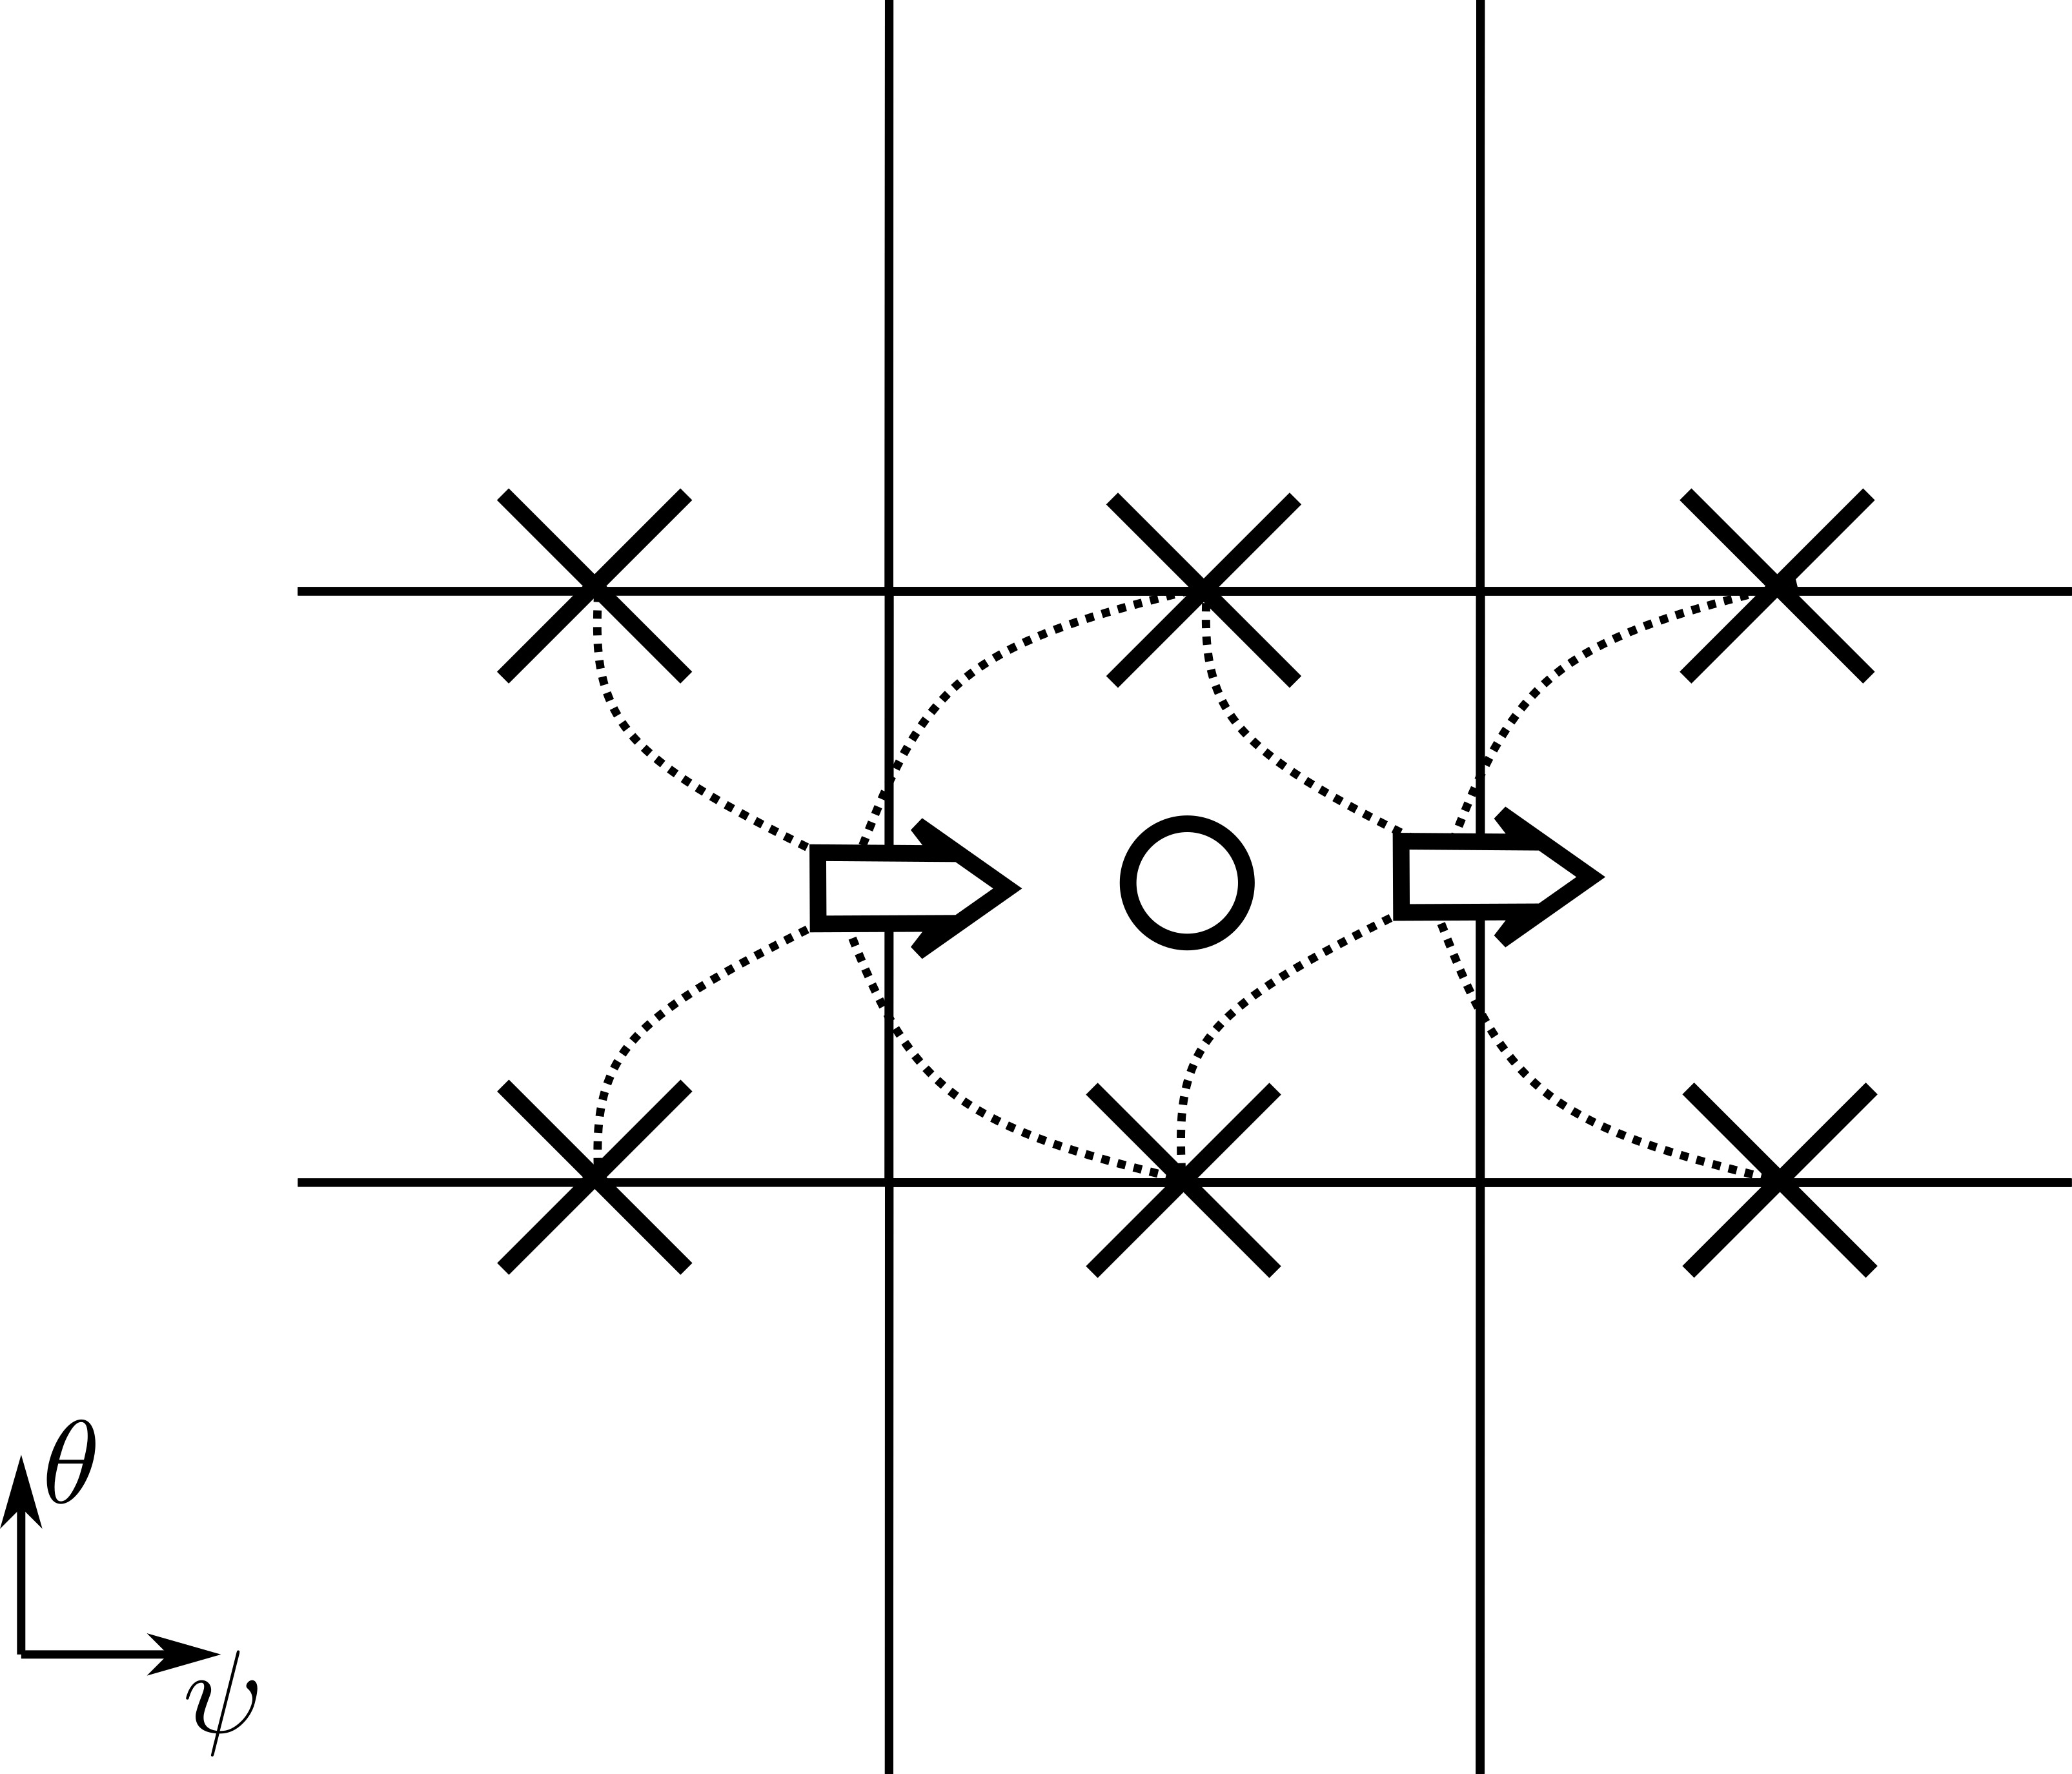
\includegraphics[height=60mm]{schemes/DivStencil_PsiTheta.jpg}
		\subcaption{Divergence in radial direction}
		\label{fig:Impl_DivPara_PsiTheta}
	\end{subfigure}
	\caption[Neighbors involved to calculated the parallel divergence]{Neighbors involved to calculated the parallel divergence. The arrows indicate the in- and outgoing fluxes that need to be calculated, and the dashed lines connect the arrows to the staggered points they require.}
	\label{fig:Impl_DivPara}
\end{figure}



\subsubsection{Perpendicular Laplacian}

Ampère's law requires the perpendicular Laplacian on the staggered grid to link $j_\parallel$ and $A_\parallel$, two staggered fields.

\begin{equation}
	\left[\grad\cdot\grad_{\perp}X^{stg}\right]^{stg}_{[i_\psi,i_\theta, i_\varphi]}
\end{equation}

Let us consider a staggered cell over the regular mesh, depicted in red in Fig. \ref{fig:StaggeredCell}. Since the Laplacian operator can be treated as a divergence of a gradient, the task . Each flux $F^{Y,i}$ is defined as the perpendicular gradient at the corresponding cell face, approximated with finite differences. The metric and diffusion coefficients $JD(g^{ij}-b^ib^j)$ are also required at the faces and we obtain them by taking their average on the closest collocated points. In poloidal and toroidal directions two collocated points shown in green in Fig. \ref{fig:StaggeredFluxTheta} and Fig. \ref{fig:StaggeredFluxPhi} are sufficient but in radial direction we need to consider eight points around the face to calculate the correct coefficients. \\

\begin{figure}[H]
	\centering
	\begin{subfigure}[b]{0.24\textwidth}
		\centering
		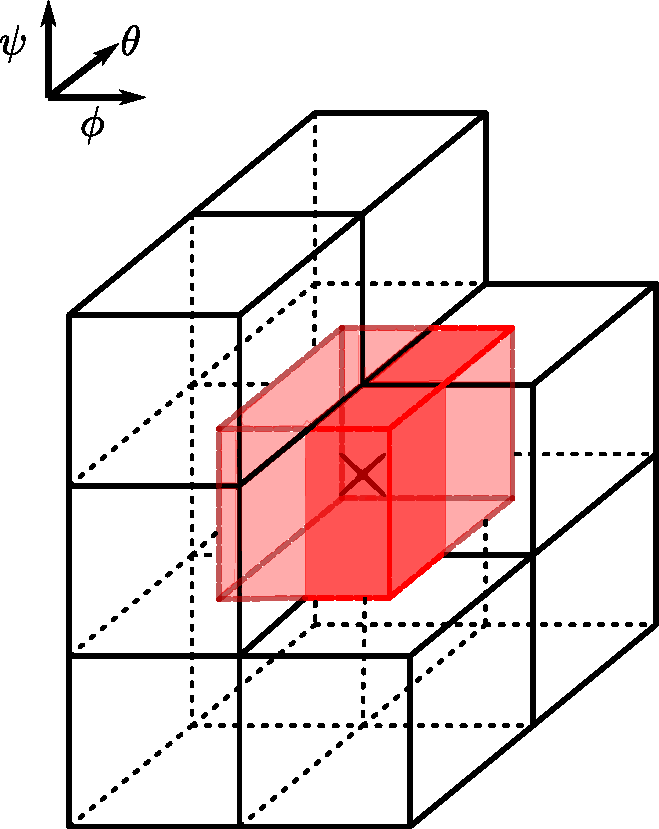
\includegraphics[width=1\textwidth]{schemes/BoundingBoxStaggeredPoint.pdf}
		\subcaption{Cell boundaries \\ for the staggered \\ grid point}
		\label{fig:StaggeredCell}
	\end{subfigure}
	\begin{subfigure}[b]{0.24\textwidth}
		\centering
		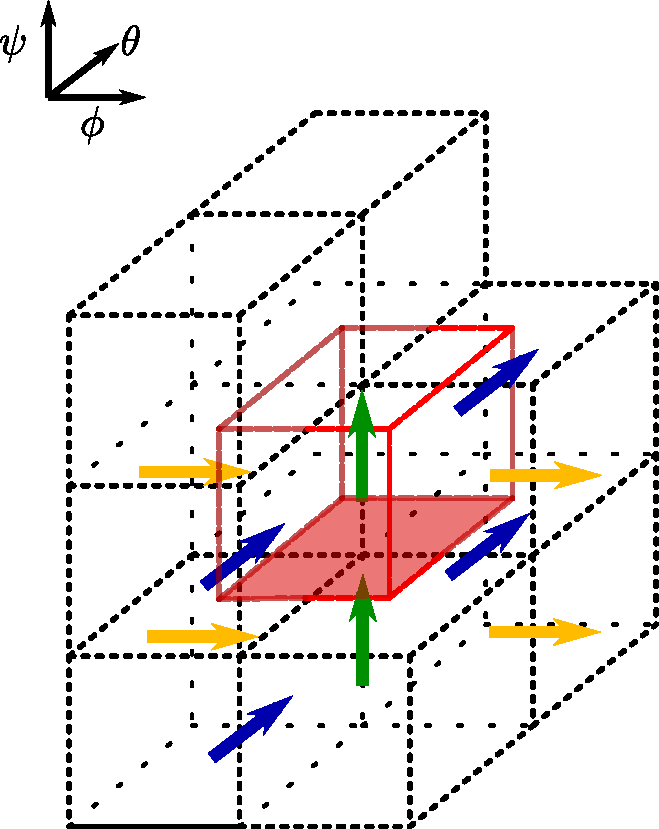
\includegraphics[width=1\textwidth]{schemes/BoundingBoxFluxPsiDiffPerp.pdf}
		\subcaption{Gradients \\ for fluxes \\ in $\psi$-direction} 
		\label{fig:StaggeredFluxPsi}
	\end{subfigure}
	\begin{subfigure}[b]{0.24\textwidth}
		\centering
		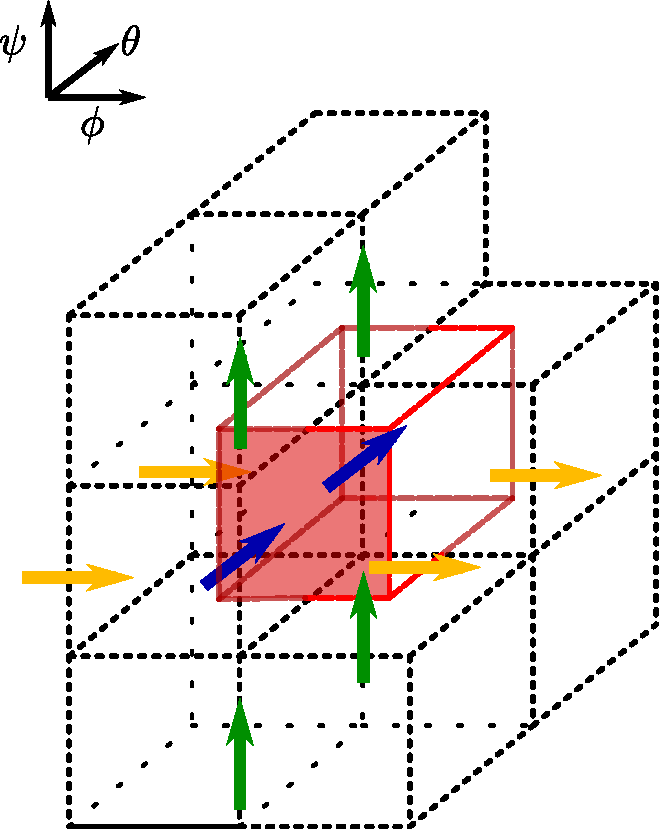
\includegraphics[width=1\textwidth]{schemes/BoundingBoxFluxThetaDiffPerp.pdf}
		\subcaption{Gradients \\ for fluxes \\ in $\theta$-direction} 
		\label{fig:StaggeredFluxTheta}
	\end{subfigure}
	\begin{subfigure}[b]{0.24\textwidth}
		\centering
		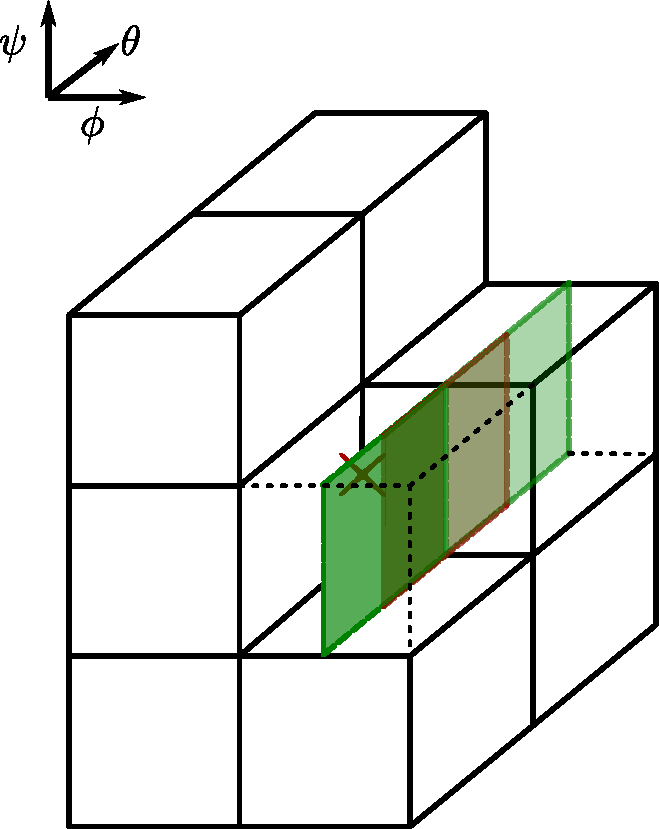
\includegraphics[width=1\textwidth]{schemes/BoundingBoxFluxPhiDiffPerp.pdf}
		\subcaption{Gradients \\ for fluxes \\ in $\varphi$-direction} 
		\label{fig:StaggeredFluxPhi}
	\end{subfigure}
	
	\caption[Depiction of the relevant cell faces to calculate fluxes of a staggered field]{Depiction of the relevant cell faces to calculate fluxes of a staggered field at coordinate index $[i_\psi, i_\theta-\frac{1}{2}, i_\varphi-\frac{1}{2}]$.}
	\label{fig:StaggeredPerpendicularLaplancianCellSurfaces}
\end{figure}


\subsection{Discretization around the X-point}
\label{ssec:DiscretizationXPt}

The staggered grid has direct implications on the estimation of fluxes around mesh singularities: while for regular fields, every cell around the X-point has well-defined neighbors (see Fig. \ref{fig:CenteredXpoint}), radial fluxes in and out of staggered cells directly cross the X-point (see Fig. \ref{fig:StaggeredXpoint}). They affect the perpendicular Laplacian operator on $A_\parallel$ in Ampere's law (Eq. \ref{eq:S3X_AmpereLaw}), advection on $j_\parallel$ in Eq. \ref{eq:S3X_advectionJPara}, and the anomalous perpendicular diffusion $\mathfrak{D}_{A,j}$. To cope with the ill-defined cell faces, fluxes across the X-point are forced to 0 by Neumann-like boundary conditions. Neighbors of the involved cells must be defined separately from the regular cells with the same index. \newline

\begin{figure}[H]
	\centering
	\begin{subfigure}[t]{0.48\textwidth}
		\centering
		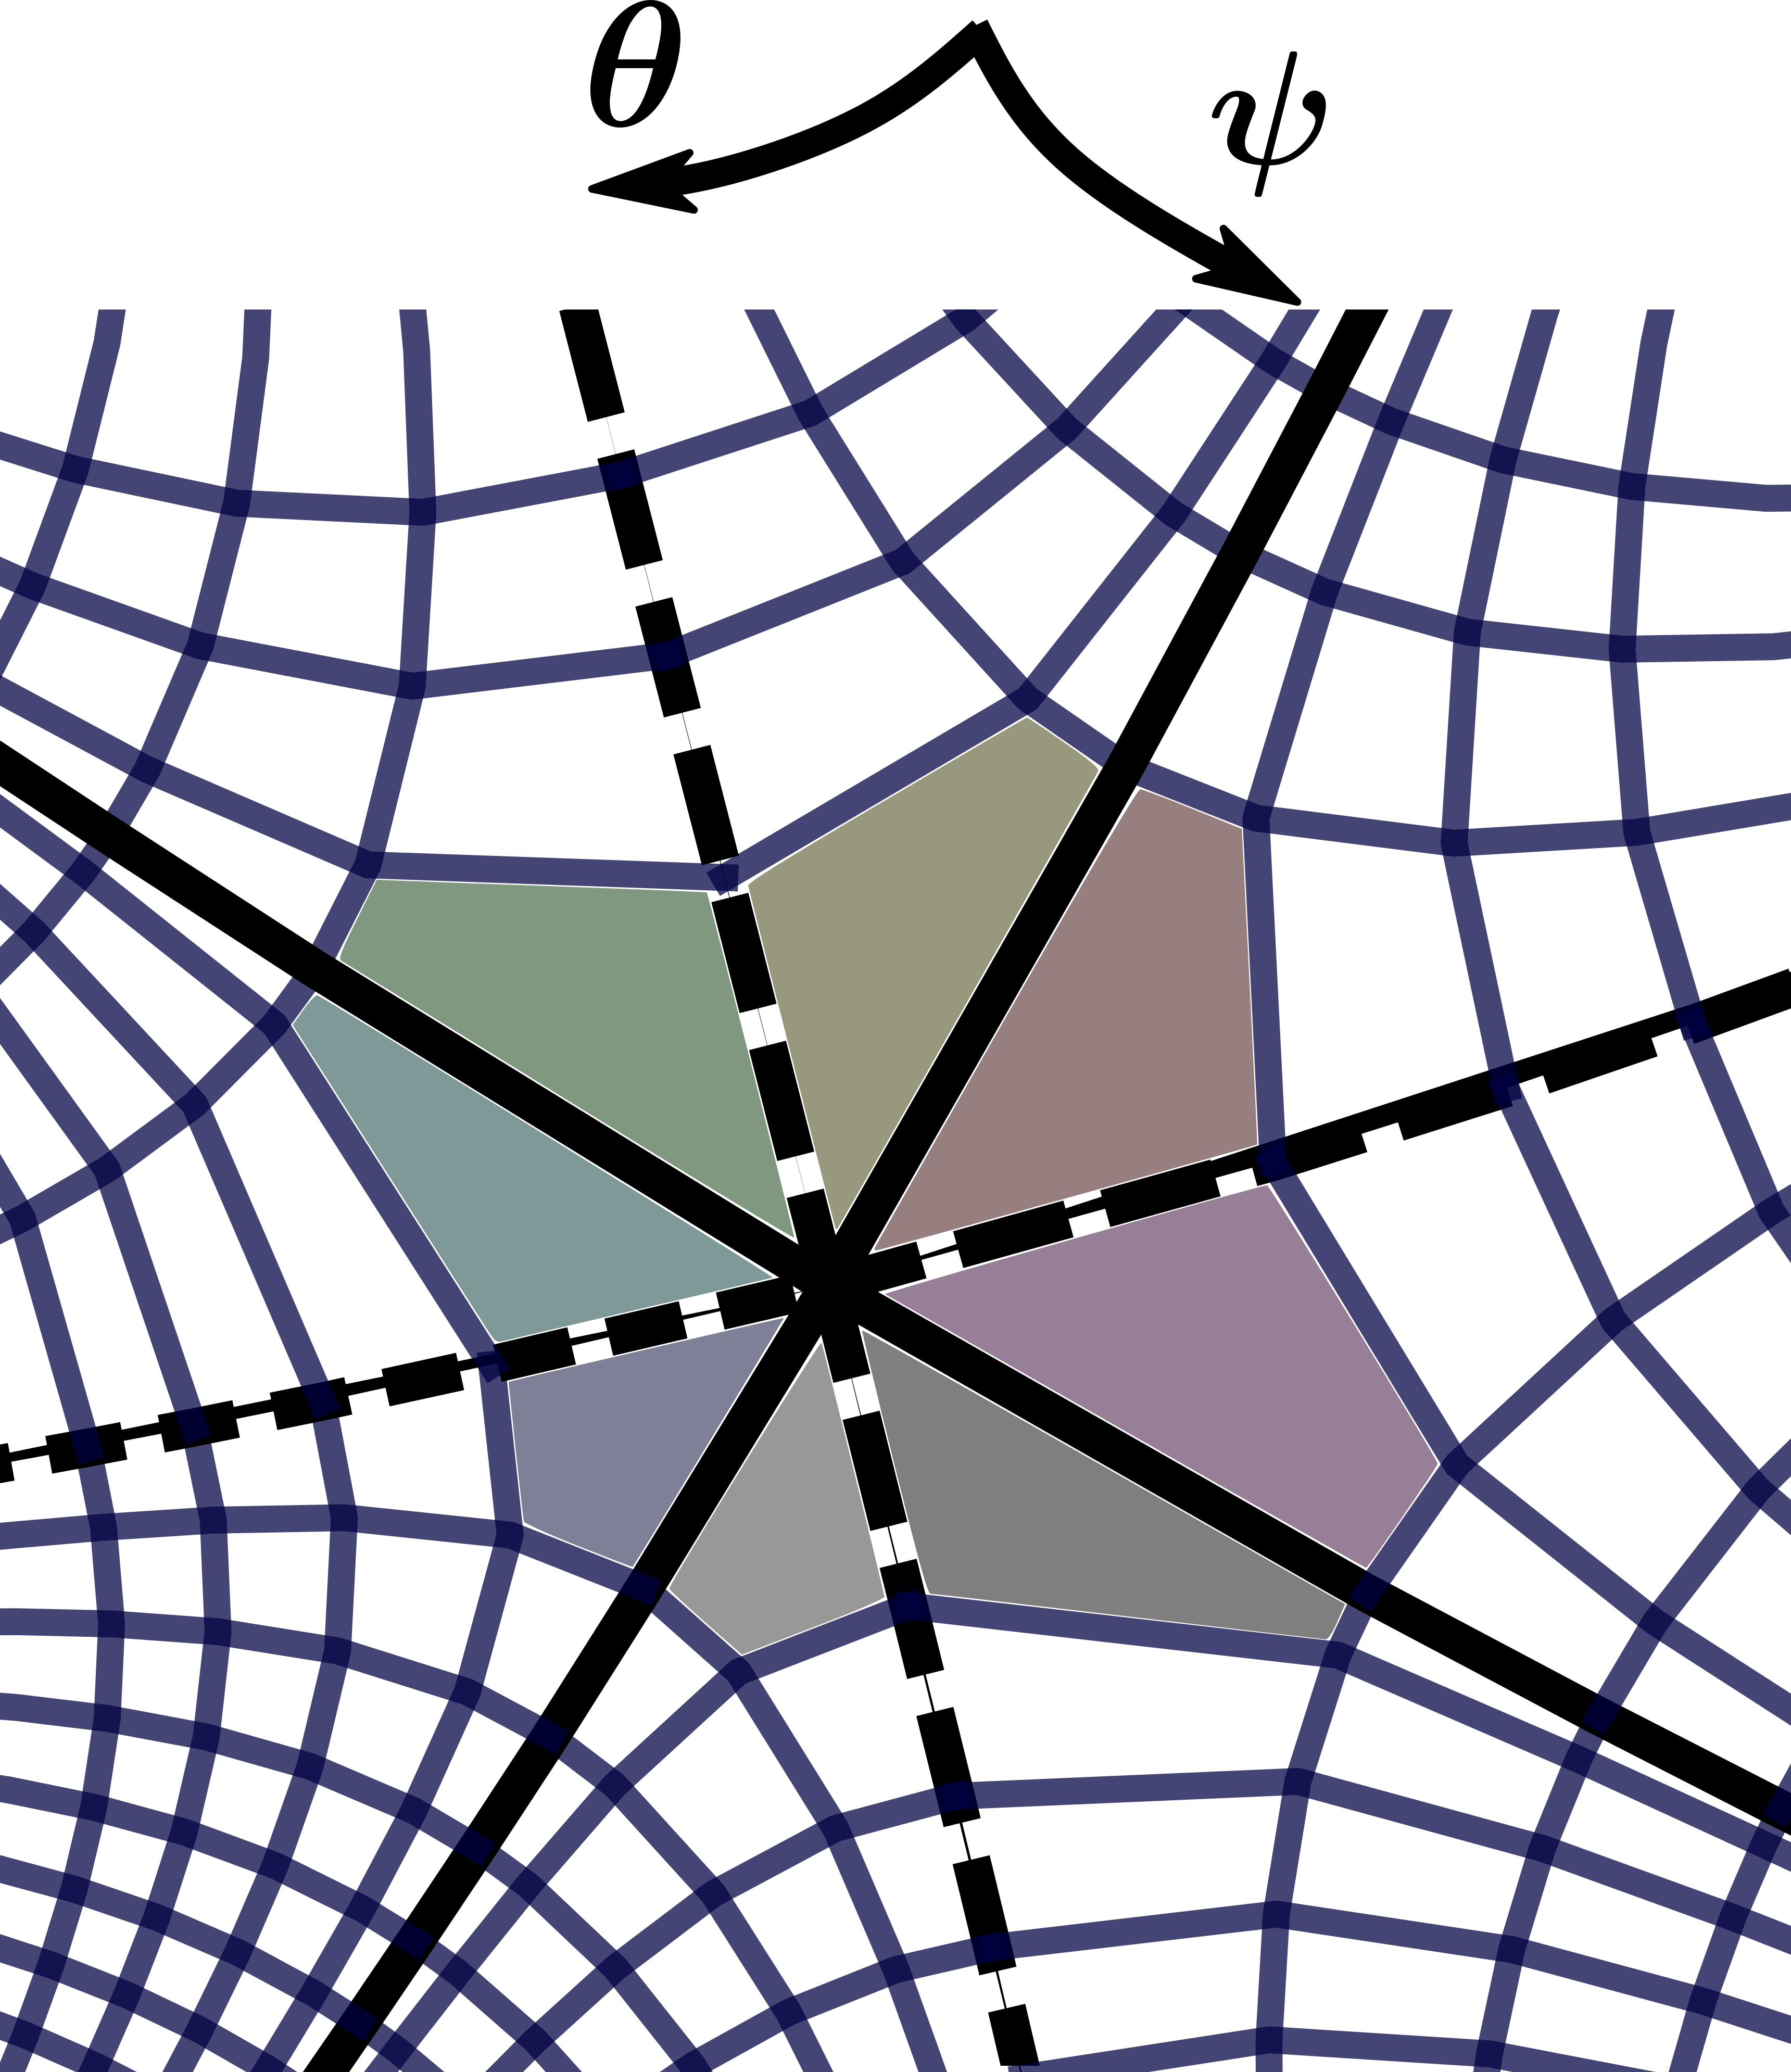
\includegraphics[height=7cm]{schemes/XpointCentered.png}
		\subcaption{View of collocated cells}
		\label{fig:CenteredXpoint}
	\end{subfigure}
	\begin{subfigure}[t]{0.48\textwidth}
		\centering
		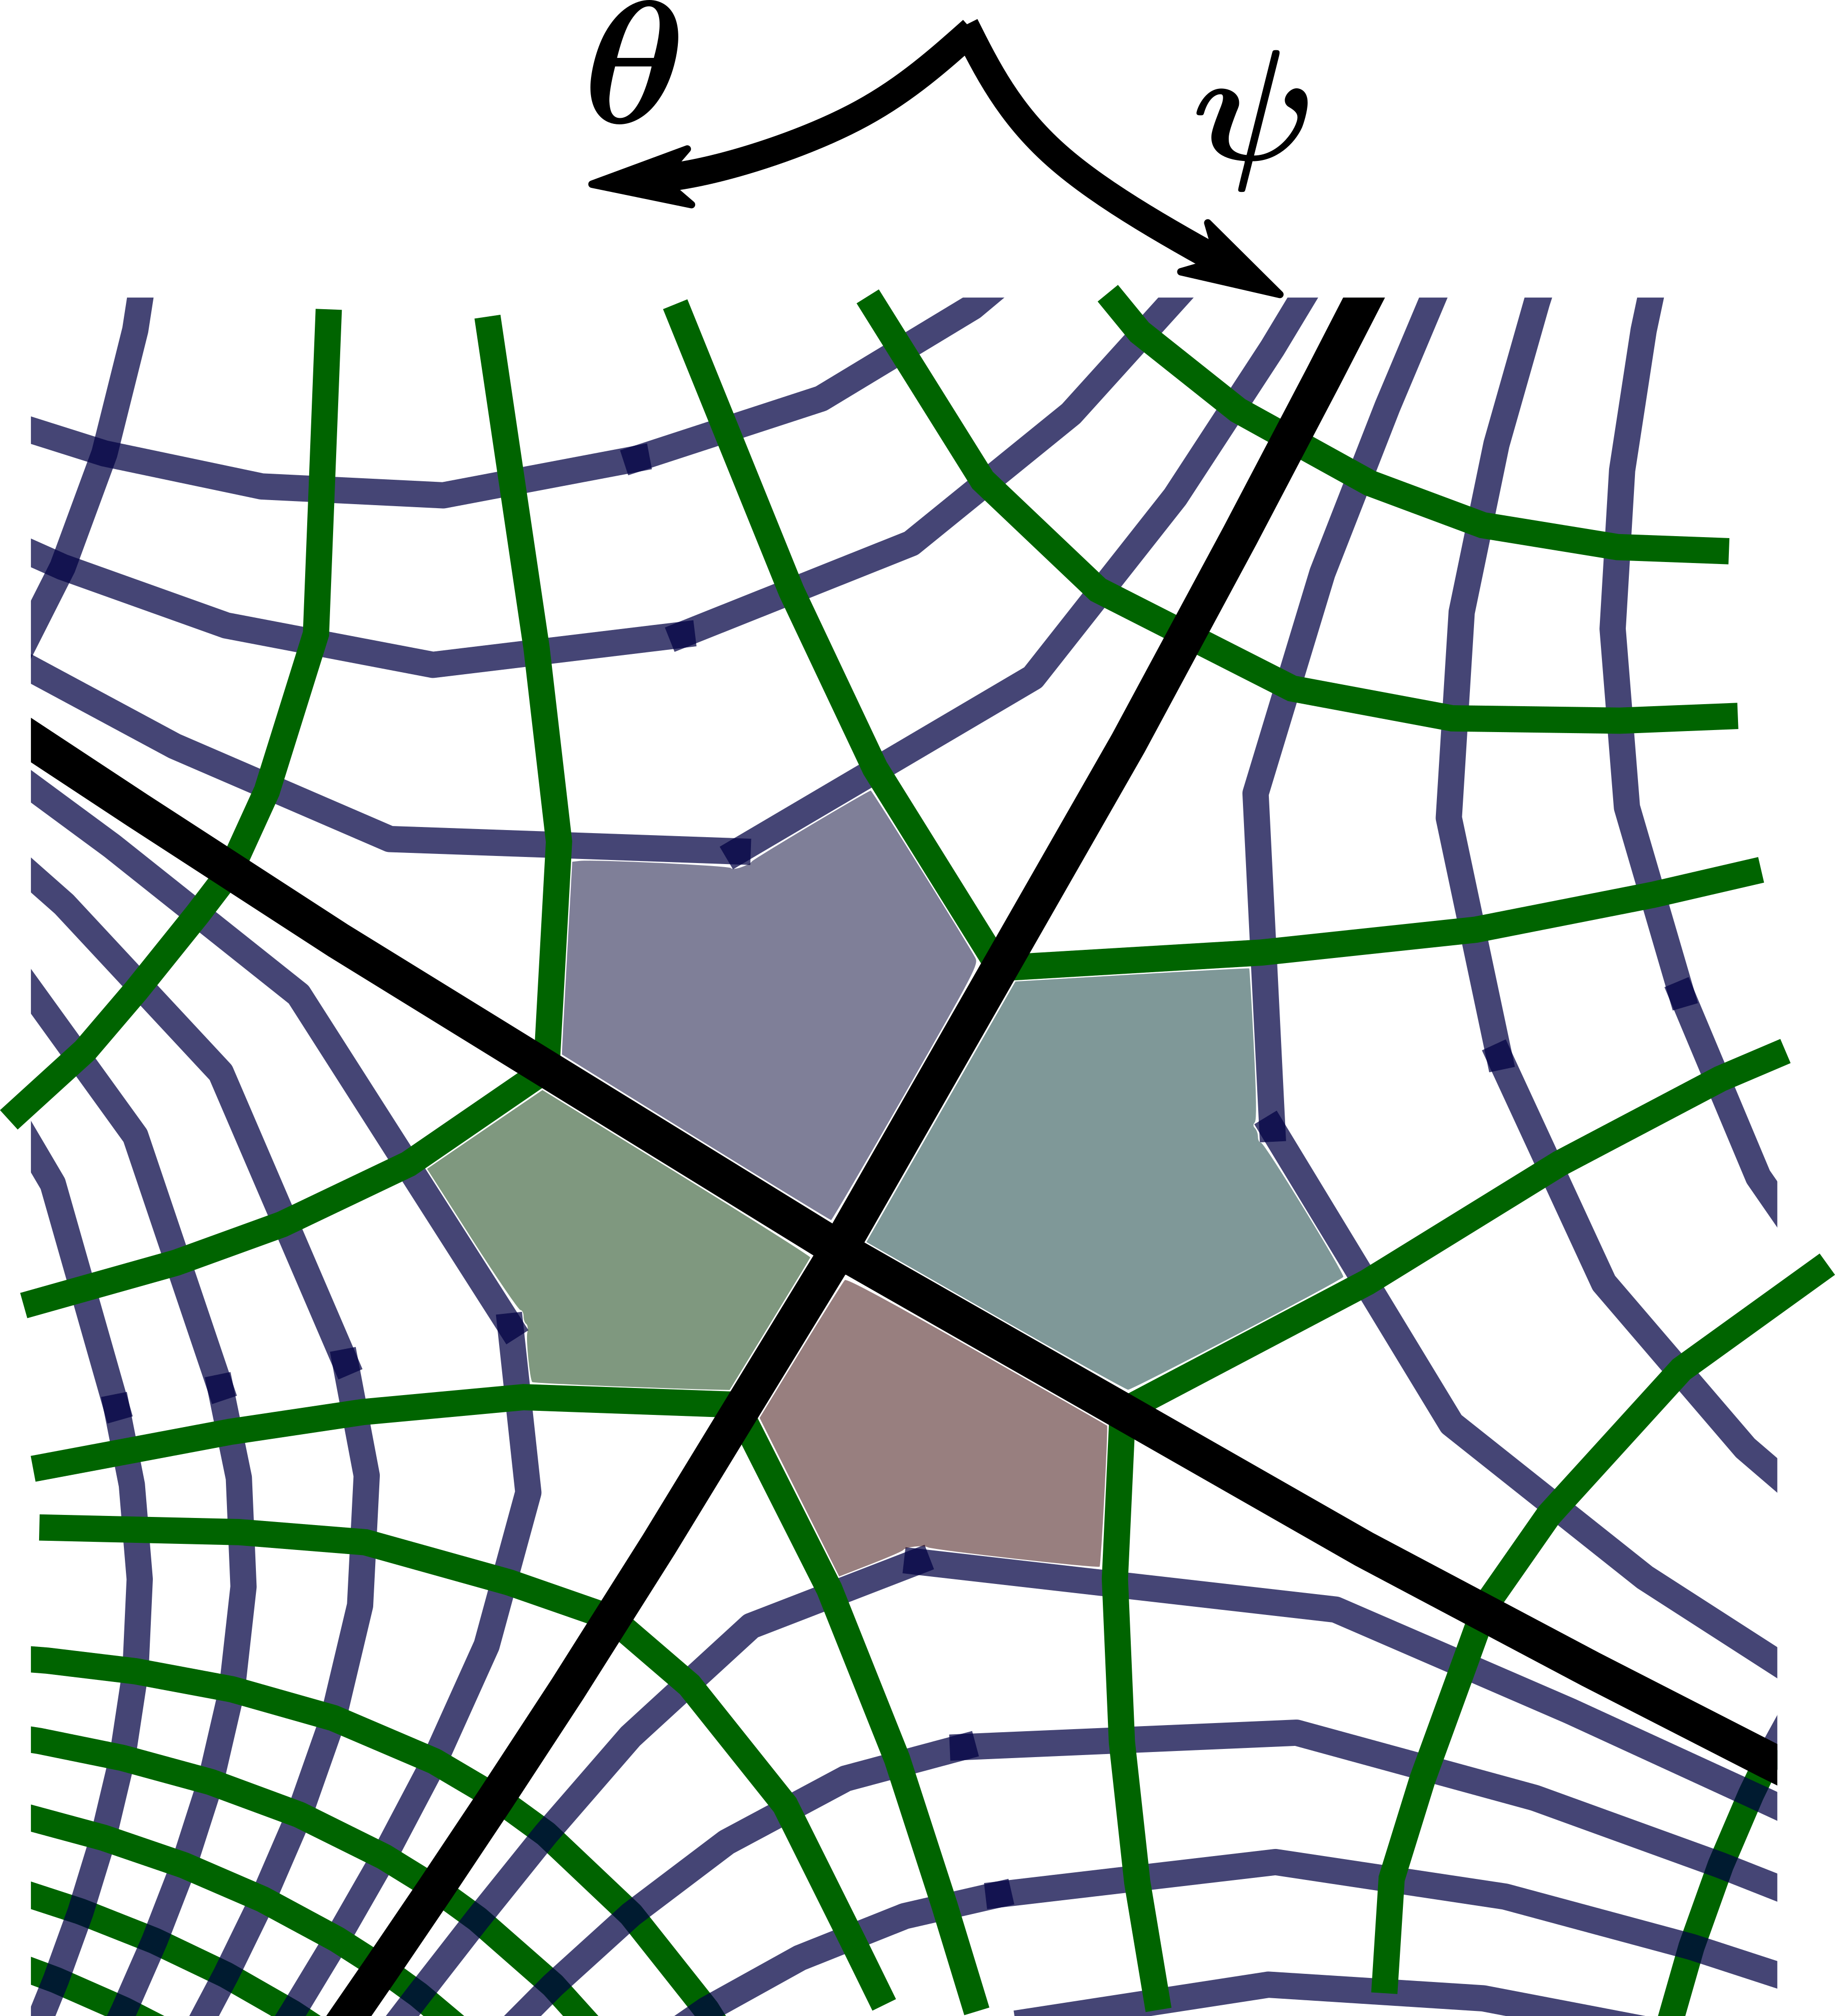
\includegraphics[height=7cm]{schemes/XpointStaggered.png}
		\subcaption{View of staggered cells}
		\label{fig:StaggeredXpoint}
	\end{subfigure}
	\caption[Sketches of the mesh around the X-point]{ Sketches of the mesh around the X-point. For collocated cells (a), 8 cells touch the X-point at a corner. For staggered cells (b), the X-point is located at the radial face of 4 cells, effectively modifying the shape of the cells to pentagons. Fluxes across the involved faces are hence ill-defined. }
	\label{fig:XpointDiscretization}
\end{figure}










\section{Electromagnetic vorticity system}
\label{sec:impl_EMvorticity}

The newly introduced fields $j_\parallel$ and $A_\parallel$ are solved implicitly along with the electric potential $\Phi$. As we face a coupled system that connects all points in the domain, direct solvers such as PASTIX are not suitable, especially for fine 3D meshes. We instead prefer to use iterative solvers available in the the PETSc or HYPRE libraries. For the original vorticity system, the Stabilized version of the Biconjugate Gradient method (BiCGStab) along with the Geometric Algebraic Multigrid (GAMG) preconditionner proved to be very efficient and it is desirable to use them on the new systems. This section describes some special numerical features in the construction of the system to facilitate the convergence of the above iterative scheme. Sec. \ref{ssec:equilibrationBLockMatrices} introduces specific row and column scaling to equilibrate the blocks in the new system and Sec. \ref{ssec:StaggeredFieldsMatrix} describes how to handle staggered fields to be compatible with the iterative scheme.

\subsection{Matrix formulation of the electromagnetic system}

With the values for $n_e$ and $T_e$ known at time-step $n+1$, the vorticity equation (Eq. \ref{eq:S3X_vorticityEquation_FullElectromagnetic}) corresponds to a 3D costly system involving $\Phi$, $j_\parallel$, and $A_\parallel$. To solve it efficiently, the advection of $j_\parallel$ and the anomalous perpendicular diffusion are treated explicitly. Following the discussion in Sec. \ref{sec:S3X_formulationEMsystem}, we integrate Ohm's law into the vorticity equation and Ampère's law. Then, at time-step $n+1$, the following dimensionless system coupling the two potentials $\Phi$ and $A_\parallel$ must be solved: \\

\begin{align}
	\begin{pmatrix}
		\nabla \cdot \left[ D_\perp \nabla_\perp \circ \right] + \nabla \cdot \left[ D_\parallel \nabla_\parallel \circ \mathbf{b} \right]  
		& \frac{\beta_0}{\delta_t} \nabla \cdot \left[ D_\parallel \circ \mathbf{b} \right] \\
		D_\parallel \nabla_\parallel \circ &
		\frac{\beta_0}{\delta_t} D_\parallel \circ - \nabla \cdot \left[ \nabla_\perp \circ \right]
	\end{pmatrix}
	\begin{pmatrix}
		\Phi^{n+1} \\ A_\parallel^{n+1}
	\end{pmatrix} 
	= \nonumber \\
	\begin{pmatrix}
		\nabla \cdot \left[ D_t j^{n}_\parallel \mathbf{b} \right] + \text{RHS}^\Phi \\
		D_t j^{n}_\parallel + \text{RHS}^{A_\parallel}
	\end{pmatrix}
	\label{eq:impl_implicitVorticitySystem}
\end{align}

with $D_\perp = \frac{m_i n_i}{B^2 \delta_t}$, $D_\parallel = \frac{1}{\eta_\parallel + \mu}$, $D_t = \frac{\mu}{\eta_\parallel + \mu}$, and $\mu = m_e / (n_e \delta_t)$ accounting for electron inertia effects. The parameter $\delta_t$ derives from the integration scheme and is equal to the time-step in the case of a first-order implicit Euler scheme. \newline

Since $\eta_\parallel \propto T_e^{-1.5}$, the parallel resistivity $\eta_\parallel$ is often a small parameter that leads to strong anisotropy between the perpendicular and parallel Laplacian operators. However, the electron inertia term, being implemented in the current solver, acts as an upper limit for the parallel diffusion coefficient, which is expected to improve the matrix conditioning as $\eta_\parallel$ approaches zero. This is in contrast to the original electrostatic model from \cite{Bufferand2021}. \newline


\subsubsection{Equilibration of the Matrix Blocks}
\label{ssec:equilibrationBLockMatrices}
Apart of the use of dimensionless quantities, no effort was made so far to ensure that the blocks in the electromagnetic matrix (Eq. \ref{eq:impl_implicitVorticitySystem}) are roughly of the same order of the magnitude, which is important for the condition number of the matrix, nor that the matrix is diagonally dominant, which is generally a desirable feature for fast convergence of iterative schemes. \\

In the following bits, we introduce some column $c_X$ and row $r_X$ scaling factors that are specific to the blocks $X$ of the matrix such that the above conditions are fullfilled as well as possible. To ensure a correct solution, the row scaling factor $r_X$ must be applied to the corresponding entry in the RHS vector. As a matter of fact, in the original vorticity matrix, we already have $r_\Phi = J$ the metrical Jacobian from Sec. \ref{ssec:MetricCurvilinearCoordinates} to remove the effect of different mesh sizes in the domain on the discrete Laplacian operators. The column scaling factors $c_X$ must be taken care of when retrieving the fields from the numerical solution and it is strongly recommended to apply them to the initial guess for the iterative scheme. \\ 

Some strategies exist to optimize the scaling task\cite{sinkhorn1967concerning,parlett1969balancing}. However, they all require an expensive matrix analysis phase that must be repeated regularly since the system changes with the progress of the simulation. Therefore, we use the knowledge about the construction of the matrix blocks to define sufficiently good scaling factors. An educated row and column scaling can considerably improve the condition number of a matrix\cite{van1969condition}. In fact, we do not want the perfect scaling to minimize the condition number (which would be as expensive as a direct solver), but give the matrix the best possible shape for the subsequent use of the GAMG pre-conditioner. It was designed for positive-definite (almost) symmetric matrices\cite{brandt1984algebraic} as they occur in elliptic PDEs and performs reasonably for diffusion-dominated parabolic problems. Note that the two diagonal blocks already have a convenient shape, and the anti-diagonal blocks contain parallel divergence and gradient operators, whose discrete stencils are almost equal and somewhat similar to the off-diagonal elements of a discrete Laplacian operator. Therefore, by scaling the second column with $c_A = \sqrt{\delta_t / \beta_0}$ and the second row with $r_A = -J\sqrt{\delta_t / \beta_0}$ the resulting matrix becomes almost symmetric and well-suited for GAMG. The minus sign is important to have the same sign for the Laplacians on $\Phi$ and $A_\parallel$, ensuring global positive definiteness, and to make the off-diagonal truly symmetric. The scalings $r_\Phi = J$ and $c_\Phi = 1$ remain unchanged from the original vorticity implementation.


\subsubsection{Staggered Fields in the Matrix}
\label{ssec:StaggeredFieldsMatrix}

The GAMG multigrid solves the system on different coarser levels by restricting the matrix and the RHS vector and then interpolates the solution back to the finer levels. In the new system, two consecutive entries belong to different fields, which makes the whole restriction-interpolation task obsolete from the very first level since neither the solution nor the matrix entries are similar between neighbours. PETSc takes care of multiple fields in a coupled system if one defines a block size that indicates GAMG how to match corresponding entries. However, as seen in Fig. \ref{fig:impl_staggeredFieldMatrix}, the fields $A_\parallel$ is defined on a staggered grid in parallel direction as opposed to the collocated field $\Phi$. For the system it means that at each wall in negative directions, a line and column for $\Phi^1$ exists but not for the  corresponding $A_\parallel^1$. This in turn is problematic for GAMG as the blocks are globally defined and two different fields would again end up together and the total system size might even not be a multiple of the blocksize, which at all prevents the initialization of the preconditioner. As a solution, a dummy line is added to the matrix for $A_\parallel^1$ with a 1 on the diagonal that is not coupled to any other line. \\

\begin{figure}[H]
	\centering
	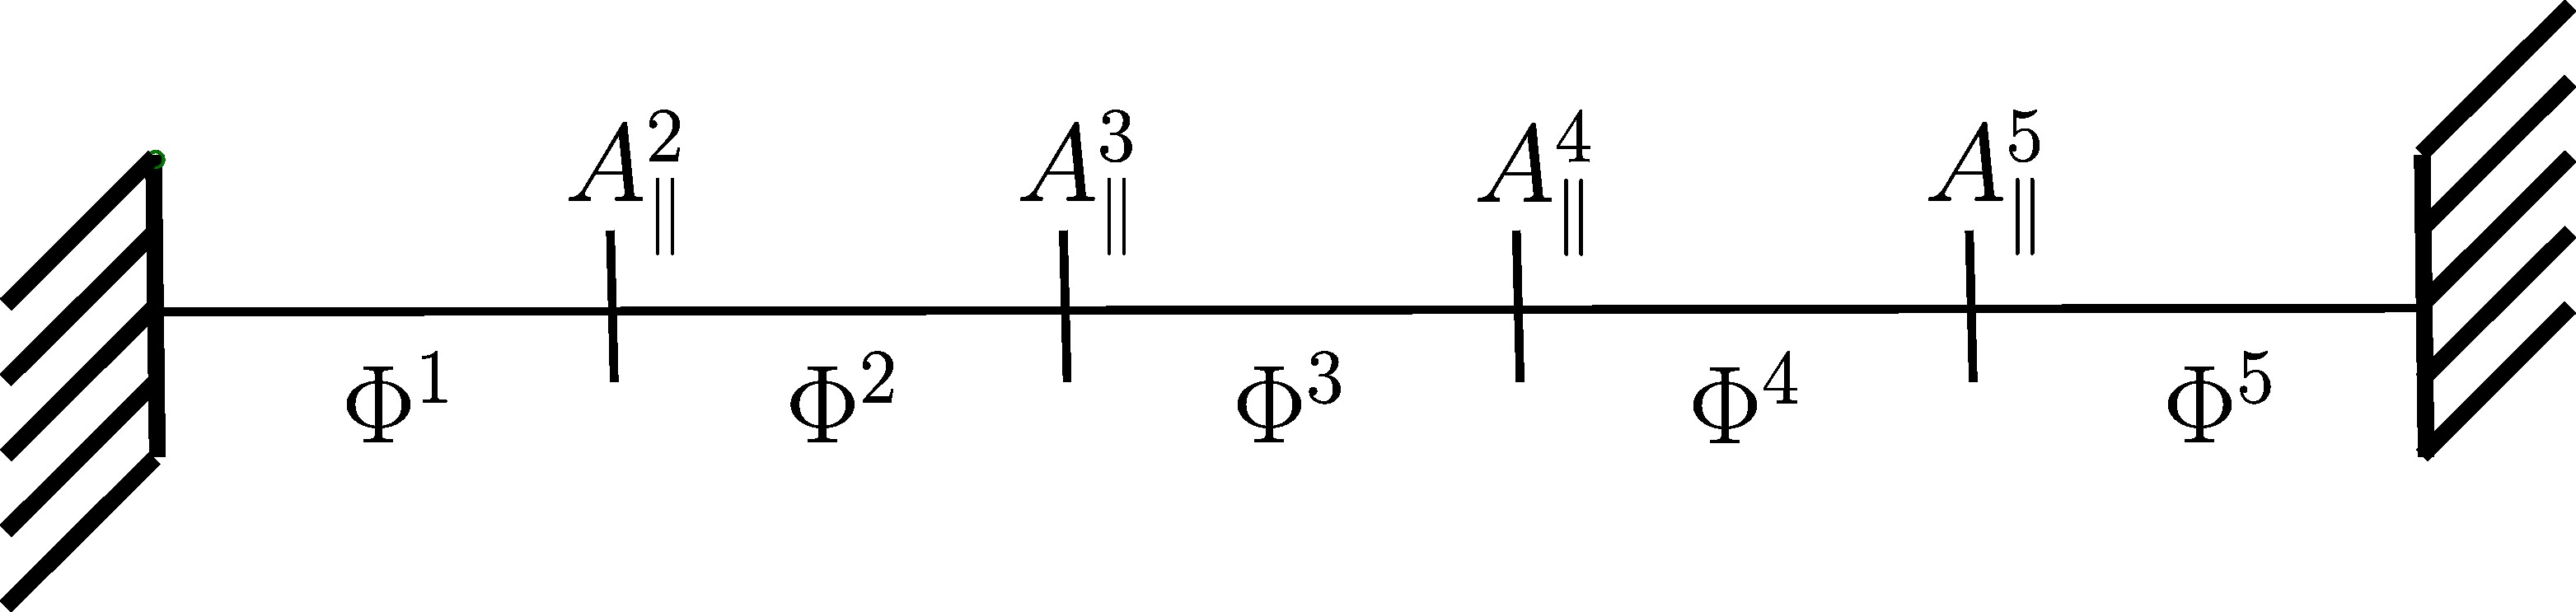
\includegraphics[width=0.9\textwidth]{schemes/staggeredMatrixLocation.jpg}
	\caption[Sketches of the mesh around the X-point]{Ordering of the fields in the vorticity equation along the $\theta$ direction}
	\label{fig:impl_staggeredFieldMatrix}
\end{figure}

It is important for GAMG to alternate entries for $A_\parallel$ and $\Phi$ in the matrix and not have one big block for each field as it reduces the distance of the non-zeros from the diagonal. It was also found that the pre-conditioner performs much better if each block is ordered $[A_\parallel^{i_\theta},\Phi^{i_\theta}]$ as the staggered grid point lies between $\Phi^{i_\theta-1}$ and $\Phi^{i_\theta}$ and the matrix ordering hence better reflects the geometrical configuration. For the geometry in Fig. \ref{fig:impl_staggeredFieldMatrix}, the matrix entries for the off-diagonal blocks would ressemble: 

\begin{equation}
	\begin{pmatrix}
		0 & \partial_\theta \\
		-\partial_\theta  & 0 
	\end{pmatrix}\begin{pmatrix}
	\Phi \\ A_\parallel
	\end{pmatrix} =
	\begin{pmatrix}
		1  & & & & & &     \\		
		   & & 1 & & & & & \\
		& 1 & & -1 & & & & \\
		& & -1 & & 1 & & & \\
		& &  & \ddots & & \ddots & & \\
		& & & & 1 & & -1 & \\
		& & & & & -1 & & 1 \\
	\end{pmatrix}
	\begin{pmatrix}
		A_\parallel^1    \\
		\Phi_\parallel^1 \\
		A_\parallel^2    \\
		\Phi_\parallel^2 \\
		\vdots           \\
		A_\parallel^5    \\
		\Phi_\parallel^5 \\		
	\end{pmatrix}
\end{equation}




\subsection{Evaluation of the condition number}

The electromagnetic vorticity system needs to be solved implicitly, and the condition number of the matrix is an important property that essentially defines the speed of convergence of iterative solvers. Extensive research over the past decade\cite{pyzara2011influence, strakos1991linear, drkovsova1995numerical, greenbaum1997numerical}, particularly on GMRES and conjugate gradient methods as they are used in SOLEDGE3X, has shown that a high condition number results in an increased number of iterations to reach convergence. The condition number of a matrix $\textbf{M}$ is defined as the ratio between its largest and smallest eigenvalues:

\begin{equation}
	\kappa\left(\textbf{M}\right) = \frac{\left|\lambda_{\text{max}}(\textbf{M})\right|}{\left|\lambda_{\text{min}}(\textbf{M})\right|}
	\label{eq:Impl_defConditionNumber}
\end{equation}

It is therefore of particular interest to investigate how the electromagnetic extension of the system affects the conditioning of the vorticity system. While there are efficient algorithms to estimate the largest eigenvalue of a matrix, the smallest is much more expensive to compute. For the large 3D vorticity system, directly calculating the condition number is not feasible. Instead, we approach this question analytically. \\

Consider a 2D orthonormal system, with perpendicular gradients exclusively in the $x$ direction and parallel gradients in the $y$ direction, with $N_x \times N_y$ discretization points. All fields are assumed to take some constant reference value, the timestep size is fixed to $\delta_t$, and time advancement is performed using the first-order implicit Euler method. Without a curvilinear grid, the gradient and divergence stencils are identical, and with the row/column scaling from Sec. \ref{ssec:equilibrationBLockMatrices}, the vorticity system can then be expressed as:


\begin{equation}
	\textbf{M} = 
	\begin{pmatrix}
		\alpha \textbf{L}_\perp + \sigma \textbf{L}_\parallel & \gamma \textbf{G}_\parallel \\ -\gamma \textbf{G}_\parallel^T & \gamma^2\textbf{L}_\perp - \sigma \textbf{I} 
	\end{pmatrix}
\end{equation}

where $\alpha = \frac{m_in_i}{B^2\delta_t}$, $\sigma = \frac{1}{\eta_\parallel + \frac{m_e}{n_e \delta_t}}$, and $\gamma = \sqrt{\frac{\delta_t }{\beta_0}}$. The stencil matrices $\textbf{L}_\perp$ and $\textbf{L}_\parallel$ describe the Laplacians between the $x$ and $y$ neighbors, respectively, while $\textbf{G}_\parallel$ represents the gradient over $y$. Their matrices take the following forms:

\begin{gather}
	\begin{aligned}
	\mathbf{L}_\perp =& \begin{pmatrix}
		-2 & 1 & 0 & \cdots & 0 \\
		1 & -2 & 1 & \cdots & 0 \\
		0 & 1 & -2 & \cdots & 0 \\
		\vdots & \vdots & \vdots & \ddots & \vdots \\
		0 & 0 & 0 & \cdots & -2
	\end{pmatrix}_{N_x \times N_x} &
	\mathbf{L}_\parallel =& \begin{pmatrix}
		-2 & 1 & 0 & \cdots & 1 \\
		1 & -2 & 1 & \cdots & 0 \\
		0 & 1 & -2 & \cdots & 0 \\
		\vdots & \vdots & \vdots & \ddots & \vdots \\
		1 & 0 & 0 & \cdots & -2
	\end{pmatrix}_{N_y \times N_y} \nonumber\\
	\end{aligned} \\
	\begin{aligned}
	\mathbf{G}_\parallel = \begin{pmatrix}
		-1 & 1 & 0 & \cdots & 0 \\
		0 & -1 & 1 & \cdots & 0 \\
		\vdots & \vdots & \vdots & \ddots & \vdots \\
		1 & 0 & 0 & \cdots & -1
	\end{pmatrix}_{N_y \times N_y}
	\end{aligned}
\end{gather}

In order to make the system invertible and avoid an infinite condition number, we assume Dirichlet-0 boundary conditions in the perpendicular direction and periodic boundary conditions in the parallel direction. This can be viewed as a region of closed flux surfaces connected to a region with a very crude sheath-dominated plasma. We can compute the eigenvalues of the two Laplacians and the gradient coupling matrix exactly.

\begin{align}
	\lambda_{k_x}(\mathbf{L}_\perp) =& 4\sin^2\left(\frac{(k_x+1)\pi}{2N_x}\right)  & \lambda_{k_y}(\mathbf{L}_\parallel) =& 4\sin^2\left(\frac{k_y\pi}{N_y}\right) & \lambda_{k_y}(\mathbf{G}_\parallel) = i\sin\left(\frac{k_y\pi}{N_y}\right)
\end{align}

where $k_x\in[0,N_x-1]$ and $k_y\in[0,N_y-1]$ are indices for all eigenvalues. We observe that both parallel systems have a zero eigenvalue that corresponds to a constant mode, due to the periodic boundary conditions along the closed flux surfaces, indicating that the solution can be determined up to a constant. The perpendicular operators, with fixed boundaries, make the system invertible with a unique solution. 

Let us now evaluate the extremal eigenvalues of the diagonal blocks of $\mathbf{M}$. For the upper-left block, which contains the sum of Laplacians, the eigenvalues correspond to the combinations of $(k_x,k_y)$ such that $|\lambda_{k_x}|+|\lambda_{k_y}|$ is minimized or maximized:

\begin{align}
	\lambda_{min}(\alpha \textbf{L}_\perp + \sigma \textbf{L}_\parallel) &= \alpha\cdot\frac{\pi^2}{N_x^2} & \lambda_{max}(\alpha \textbf{L}_\perp + \sigma \textbf{L}_\parallel) &= 4(\alpha + \sigma)
	\label{eq:Impl_EVupperLeftBlock}
\end{align}

For the lower-right block matrix, the identity matrix will shift the eigenvalues of the perpendicular Laplacian by $\sigma$:

\begin{align}
	\lambda_{min}(\sigma \textbf{I} - \gamma^2 \textbf{L}_\perp) &= \sigma - 4\gamma^2 & \lambda_{max}(\gamma^2 \sigma \textbf{I} - \textbf{L}_\perp ) &= \sigma - \gamma^2\frac{\pi^2}{N_x^2}
	\label{eq:Impl_EVlowerRightBlock}
\end{align}

For sufficiently large systems, the largest eigenvalue will be on the order of $\sigma$. If $\sigma \gg \gamma^2$, all eigenvalues will be close to $\sigma$, resulting in an excellent matrix condition. However, if $\sigma < 4\gamma^2$, some eigenvalues may become negative, causing the system to lose its positive-definiteness. This can lead to strong instabilities, and standard iterative solvers (e.g., GMRES or BiCGStab) may fail or produce unreliable results, as these methods are generally designed for positive-definite matrices. To ensure that the problem remains well-posed, we must enforce the constraint:

\begin{equation}
	\frac{1}{4}\beta_0 > \delta_t\eta_\parallel + \frac{m_e}{n_e} 
	\label{eq:Impl_conditionPositiveDefinite}
\end{equation}

This condition states that $\beta_0$ cannot be too small for the system to remain solvable. Assuming this lower condition on $\beta_0$ holds with a sufficient margin, the minimum and maximum eigenvalues in Eq. \ref{eq:Impl_EVlowerRightBlock} are simply $\lambda_{min} = \lambda_{max} = \sigma$. \\

We now have all extremal eigenvalues along the block diagonal. For the combined matrix $\mathbf{M}$, the gradient coupling plays a crucial role. If the coupling is small, the eigenvalues of $\mathbf{M}$ are given by the union of the eigenvalues of the diagonal blocks. The condition number of $\mathbf{M}$ is then the ratio of the overall maximum and minimum eigenvalues of the block matrices. Since $\gamma$ is certainly smaller than $\sigma$, we should investigate the impact of the coupling in more detail. The matrix $\mathbf{M}$ can be transformed into a block diagonal form by applying the Schur complement $\mathbf{S}$ on the lower-left block.


\begin{align}
	\textbf{M} = \begin{pmatrix}
		\textbf{A} & \textbf{B} \\ -\textbf{B}^T & \textbf{C} 
	\end{pmatrix} &= \begin{pmatrix}
		\textbf{I} & 0 \\ -\textbf{B}^T\textbf{A}^{-1} & \textbf{I}
	\end{pmatrix}\begin{pmatrix}
		\textbf{A} & 0 \\ 0 & \textbf{S}
	\end{pmatrix}\begin{pmatrix}
		\textbf{I} & \textbf{A}^{-1}\textbf{B} \\ 0 & \textbf{I}
	\end{pmatrix} & \text{with: } 
	\textbf{S} = \textbf{D} + \textbf{B}^T \textbf{A}^{-1}\textbf{B}
\end{align}


The block diagonal matrix is multiplied by both a lower and an upper diagonal matrix. Since they are invertible and all diagonal elements are equal to 1, the block diagonal matrix is quasi-similar to $\textbf{M}$\cite{gallier2010schur}, thereby preserving its eigenvalues. Calculating the eigenvalues of the block diagonal matrix gives us then a good approximation for the actual eigenvalues of $\textbf{M}$. We now need to estimate the eigenvalues of the Schur complement. Given that $\textbf{A}$ is Laplacian-based, the eigenvalues of $\textbf{A}^{-1}$ are the reciprocals of the eigenvalues of $\textbf{A}$, as shown in Eq. \ref{eq:Impl_EVupperLeftBlock}. The matrix is sandwiched between the gradient operator and its transpose, and together they behave like a parallel Laplacian with the scaling factor $\gamma^2$. We can first estimate:

\begin{align}
	\lambda_{min}(\textbf{B}^T \textbf{A}^{-1}\textbf{B}) &= \frac{\gamma^2\lambda_{min}(L_\parallel)}{\lambda_{max}(\alpha \textbf{L}_\perp + \sigma \textbf{L}_\parallel)} = 0 \\ 
	\lambda_{max}(\textbf{B}^T \textbf{A}^{-1}\textbf{B}) &= \frac{\gamma^2\lambda_{max}(L_\parallel)}{\lambda_{min}(\alpha \textbf{L}_\perp + \sigma \textbf{L}_\parallel)} = \frac{4\gamma^2N_x^2}{\alpha\pi^2}
\end{align}

By combining this result with the eigenvalues of $\sigma \textbf{I} - \gamma^2 \textbf{L}_\perp$ from Eq. \ref{eq:Impl_EVlowerRightBlock}, we can estimate the extremal eigenvalues of the Schur complement:

\begin{align}
	\label{eq:Impl_EVschurComplement}
	\lambda_{min}(\textbf{S}) &= \sigma  & 
	\lambda_{max}(\textbf{S}) &= \sigma + \frac{4\gamma^2N_x^2}{\alpha\pi^2}
\end{align}

Everything is now in place to address the eigenvalues of $\mathbf{M}$ with the two block diagonals $\textbf{A}$ and $\textbf{S}$. Recall the assumption $\sigma \gg \gamma^2$ from Eq. \ref{eq:Impl_conditionPositiveDefinite}, thus the double-Laplacian system in Eq. \ref{eq:Impl_EVupperLeftBlock} defines the minimum eigenvalue of $\textbf{M}$. Considering that $\alpha \sim 1/\delta_t$ in the dimensionless equations and $\gamma^2 \sim \delta_t / \beta_0$ is large, we can reasonably expect $\gamma^2 \gg \alpha$. The maximum eigenvalue of $\textbf{M}$ arises from the Schur complement in Eq. \ref{eq:Impl_EVschurComplement}. Therefore, the condition number of $\textbf{M}$ can be estimated as:

\begin{equation}
	\label{eq:Impl_conditionNumberM}
	\kappa(\textbf{M}) \approx \frac{\sigma N_x^2}{\alpha\pi^2} + \frac{4\gamma^2N_x^4}{\alpha^2\pi^4}
\end{equation}

or in terms of dimensionless reference values:

\begin{equation}
	\label{eq:Impl_conditionNumberElectromagneticVorticitySystem}
	\boxed{
		\kappa(\textbf{M}) \approx \frac{ B^2\delta_t N_\perp^2}{m_in_i\pi^2} \cdot \frac{1}{\eta_\parallel + \frac{m_e}{n_e \delta_t}} + \frac{4\delta_t^3 B^4 N_\perp^4}{\beta_0m_i^2n_i^2\pi^4}
	}
\end{equation}

In the case of the system with electron inertia, but without electromagnetic induction, the analysis becomes much simpler as only the double Laplacian block matrix constitutes the system. Its condition number is given by the eigenvalues in Eq. \ref{eq:Impl_EVupperLeftBlock}:

\begin{equation}
	\label{eq:Impl_conditionNumberM_electronInertia}
	\kappa(\textbf{A}) = \frac{4\sigma N_x^2}{\alpha\pi^2} + \frac{4 N_x^2}{\pi^2}
\end{equation}

and is primarily determined by the first term. It can be written as:

\begin{equation}
	\label{eq:Impl_conditionNumberElectrnInertiaVorticitySystem}
	\boxed{
		\kappa(\textbf{A}) \approx \frac{ B^2\delta_t N_\perp^2}{m_in_i\pi^2} \cdot \frac{1}{\eta_\parallel + \frac{m_e}{n_e \delta_t}}
	}
\end{equation}

From these expressions for the condition number, we observe a degradation as the electric resistivity approaches zero, aligning with the difficulties faced by the original electrostatic implementation in higher-power scenarios. The finite electron mass acts as a lower bound for $\eta_\parallel$, which is expected to significantly aid iterative solvers in such scenarios. Magnetic induction introduces the second term in Eq. \ref{eq:Impl_conditionNumberElectromagneticVorticitySystem}, and will always deteriorate the matrix conditioning. However, it is inversely proportional to $\beta_0$, such that the deterioration is limited as the pressure ratio increases. Numerically, electromagnetic effects should only be considered in simulation scenarios where $\beta_0$ is sufficiently large. This point is further emphasized by the condition in Eq. \ref{eq:Impl_conditionPositiveDefinite}, which imposes a lower limit on $\beta_0$ to ensure a positive-definite matrix—an essential property for most iterative solvers. In Fig. \ref{fig:Impl_conditionNumber}, we illustrate how the condition number changes with $\eta_\parallel$, $\delta_t$, and $N_\perp$ for both electrostatic and electromagnetic systems, with and without electron inertia. 

\begin{figure}[H]
	\centering
	\begin{subfigure}[t]{0.30\textwidth}
		\centering
		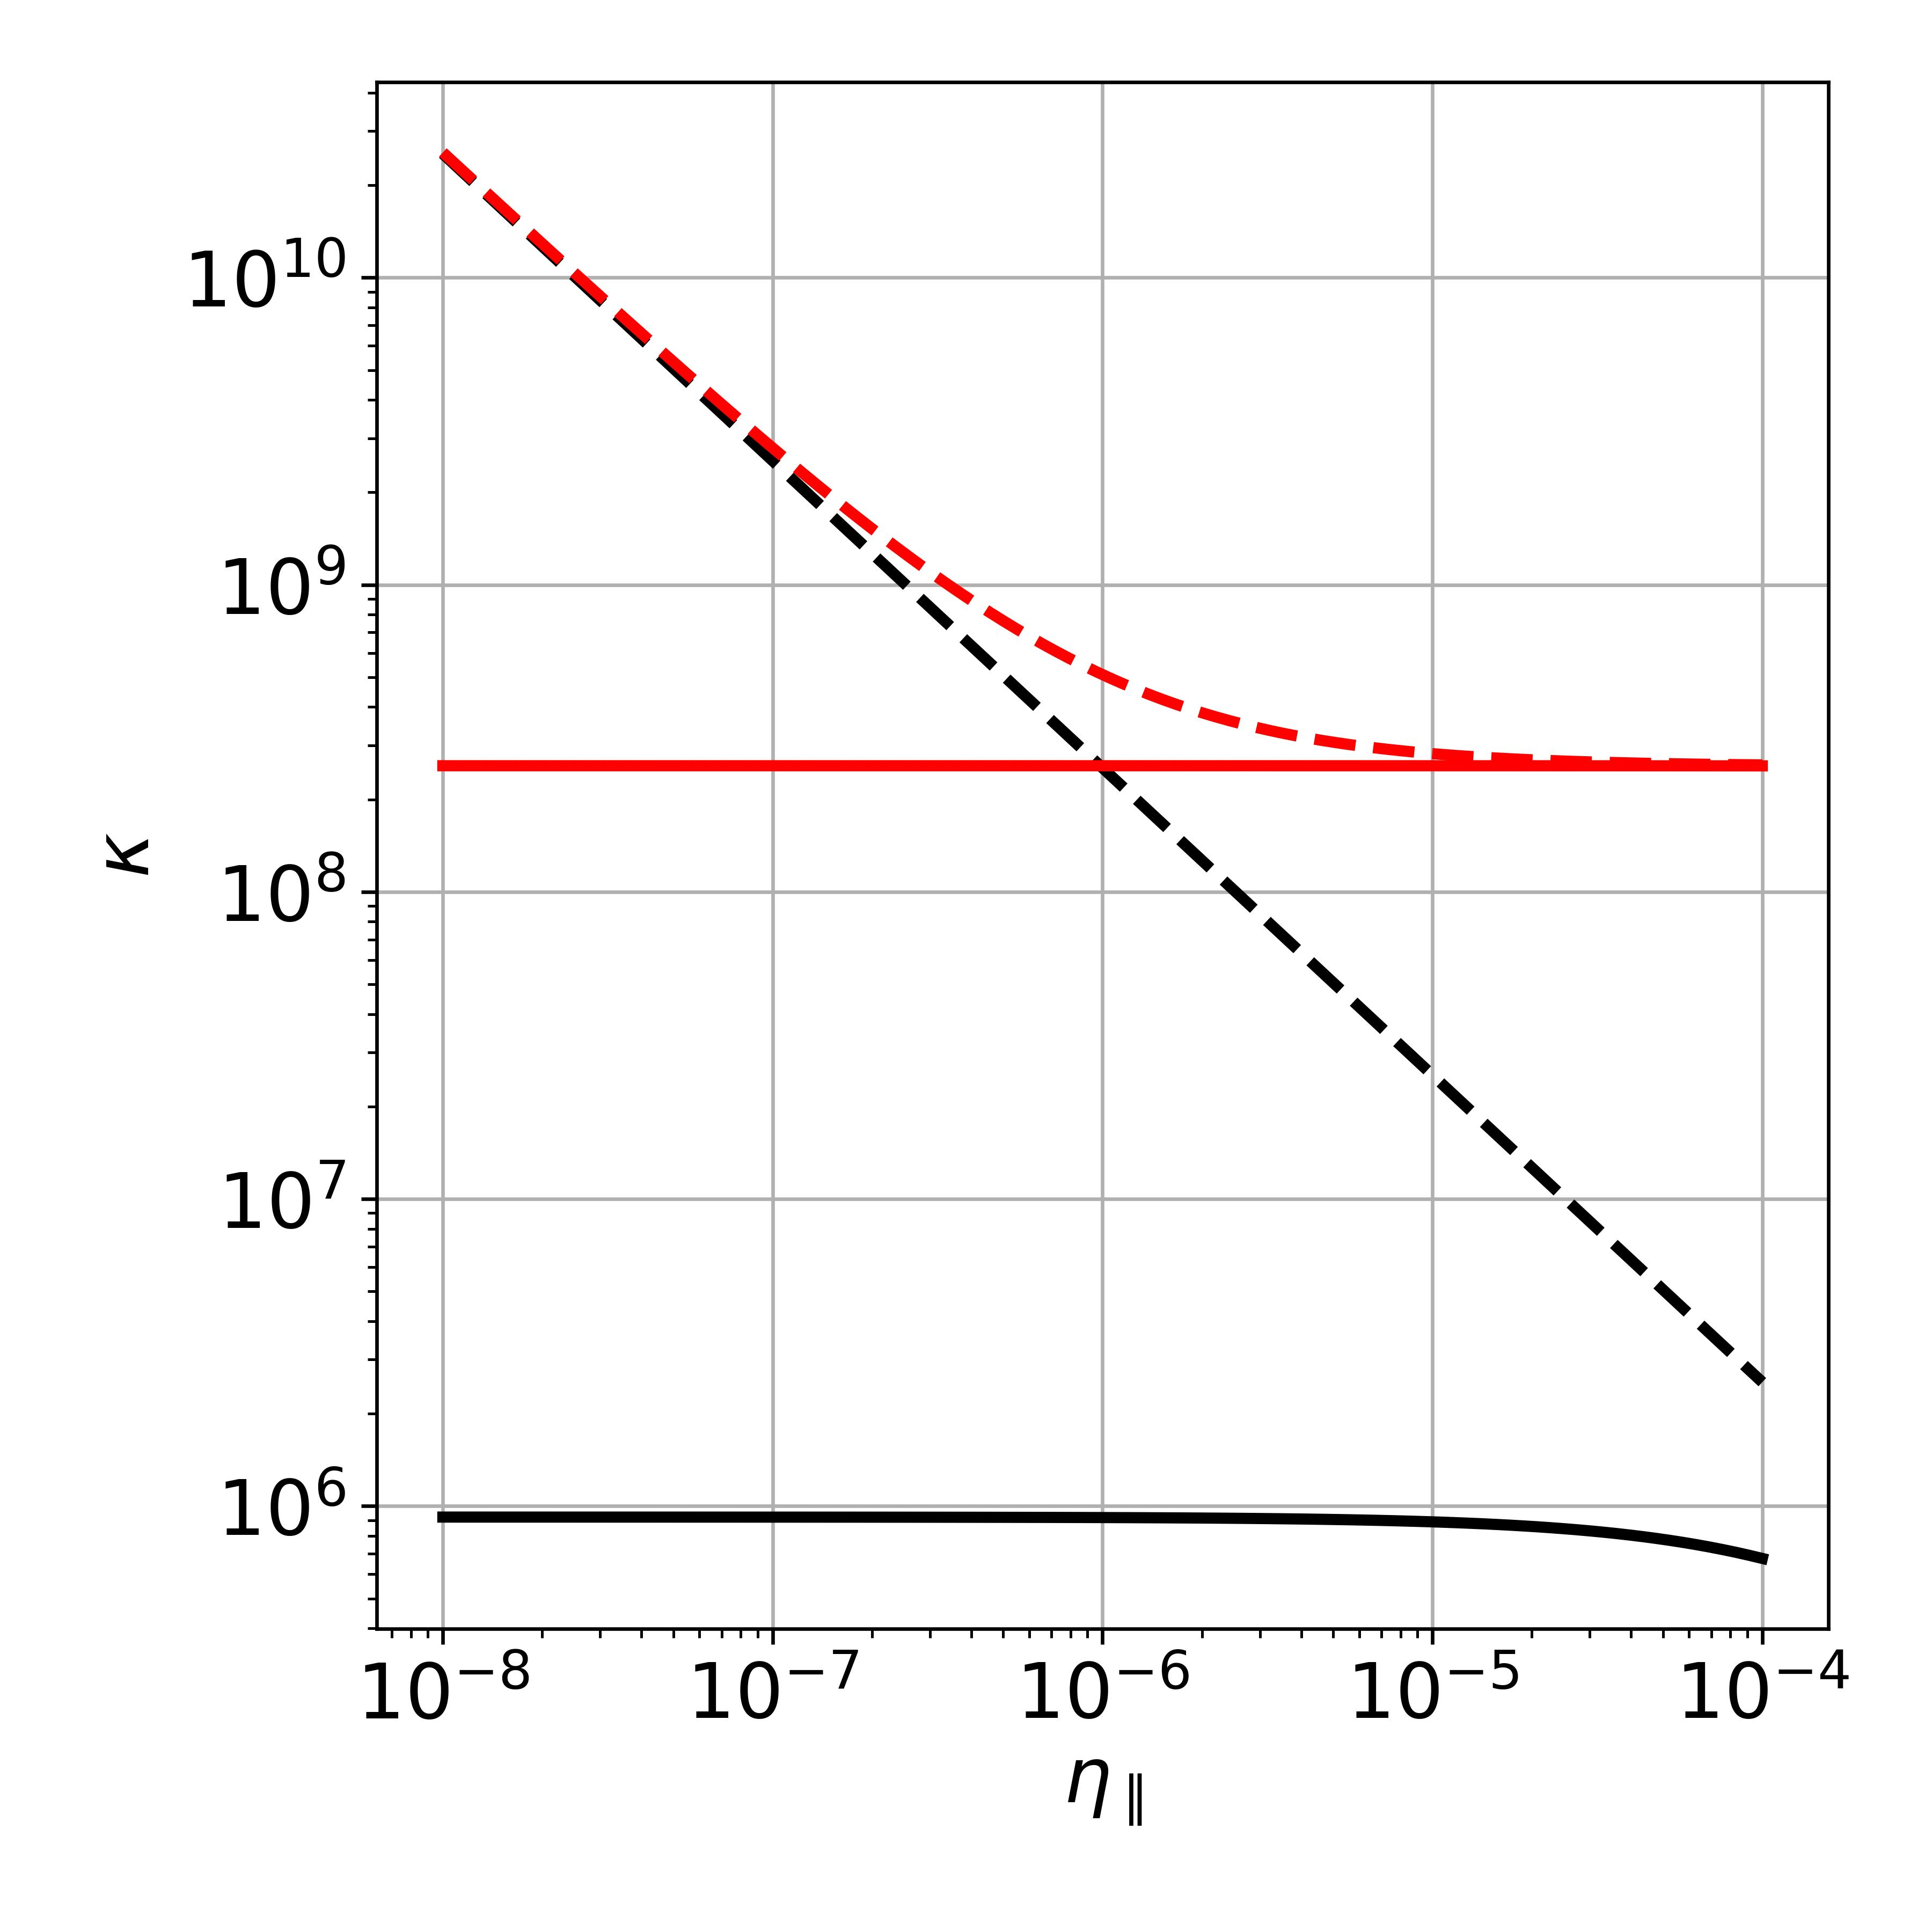
\includegraphics[width=1\textwidth]{schemes/conditionNumber_eta.jpg}
		\subcaption{Parallel electric \\ resistivity $\eta_\parallel$}
		\label{fig:Impl_conditionNumber_eta}
	\end{subfigure}
	\begin{subfigure}[t]{0.30\textwidth}
		\centering
		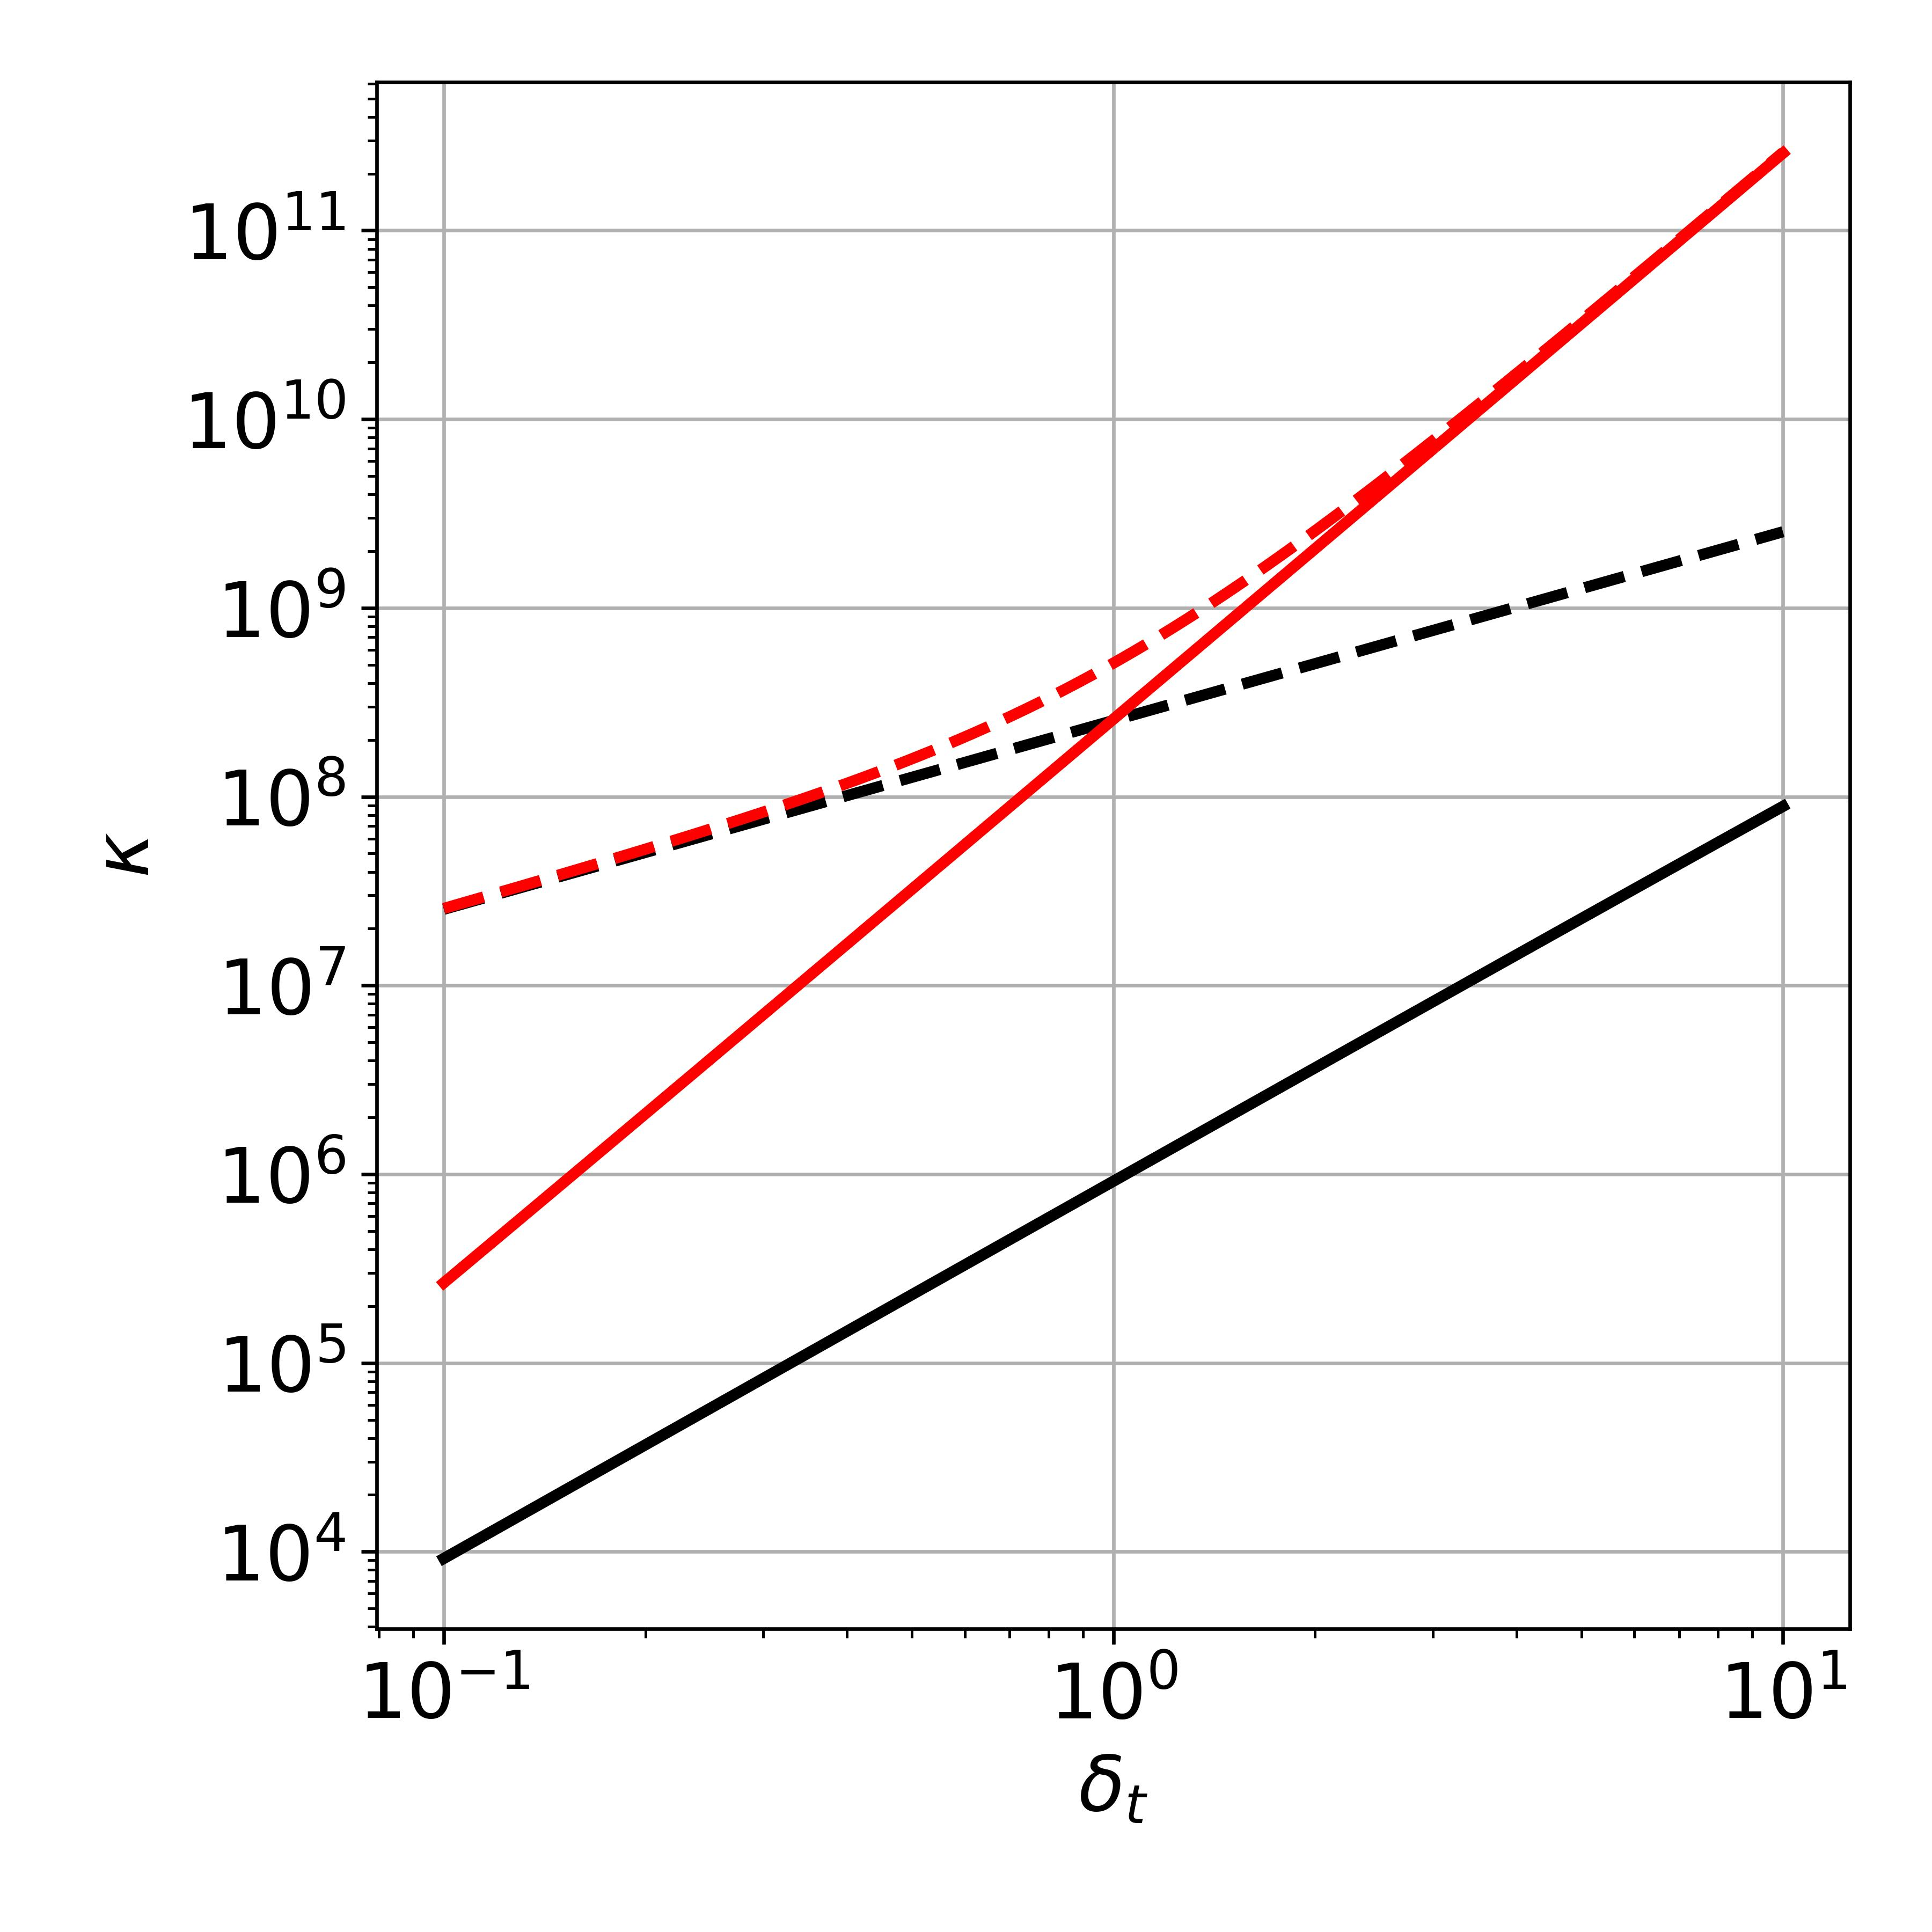
\includegraphics[width=1\textwidth]{schemes/conditionNumber_dt.jpg}
		\subcaption{Timestep size $\delta_t$}
		\label{fig:Impl_conditionNumber_dt}
	\end{subfigure}
	\begin{subfigure}[t]{0.30\textwidth}
		\centering
		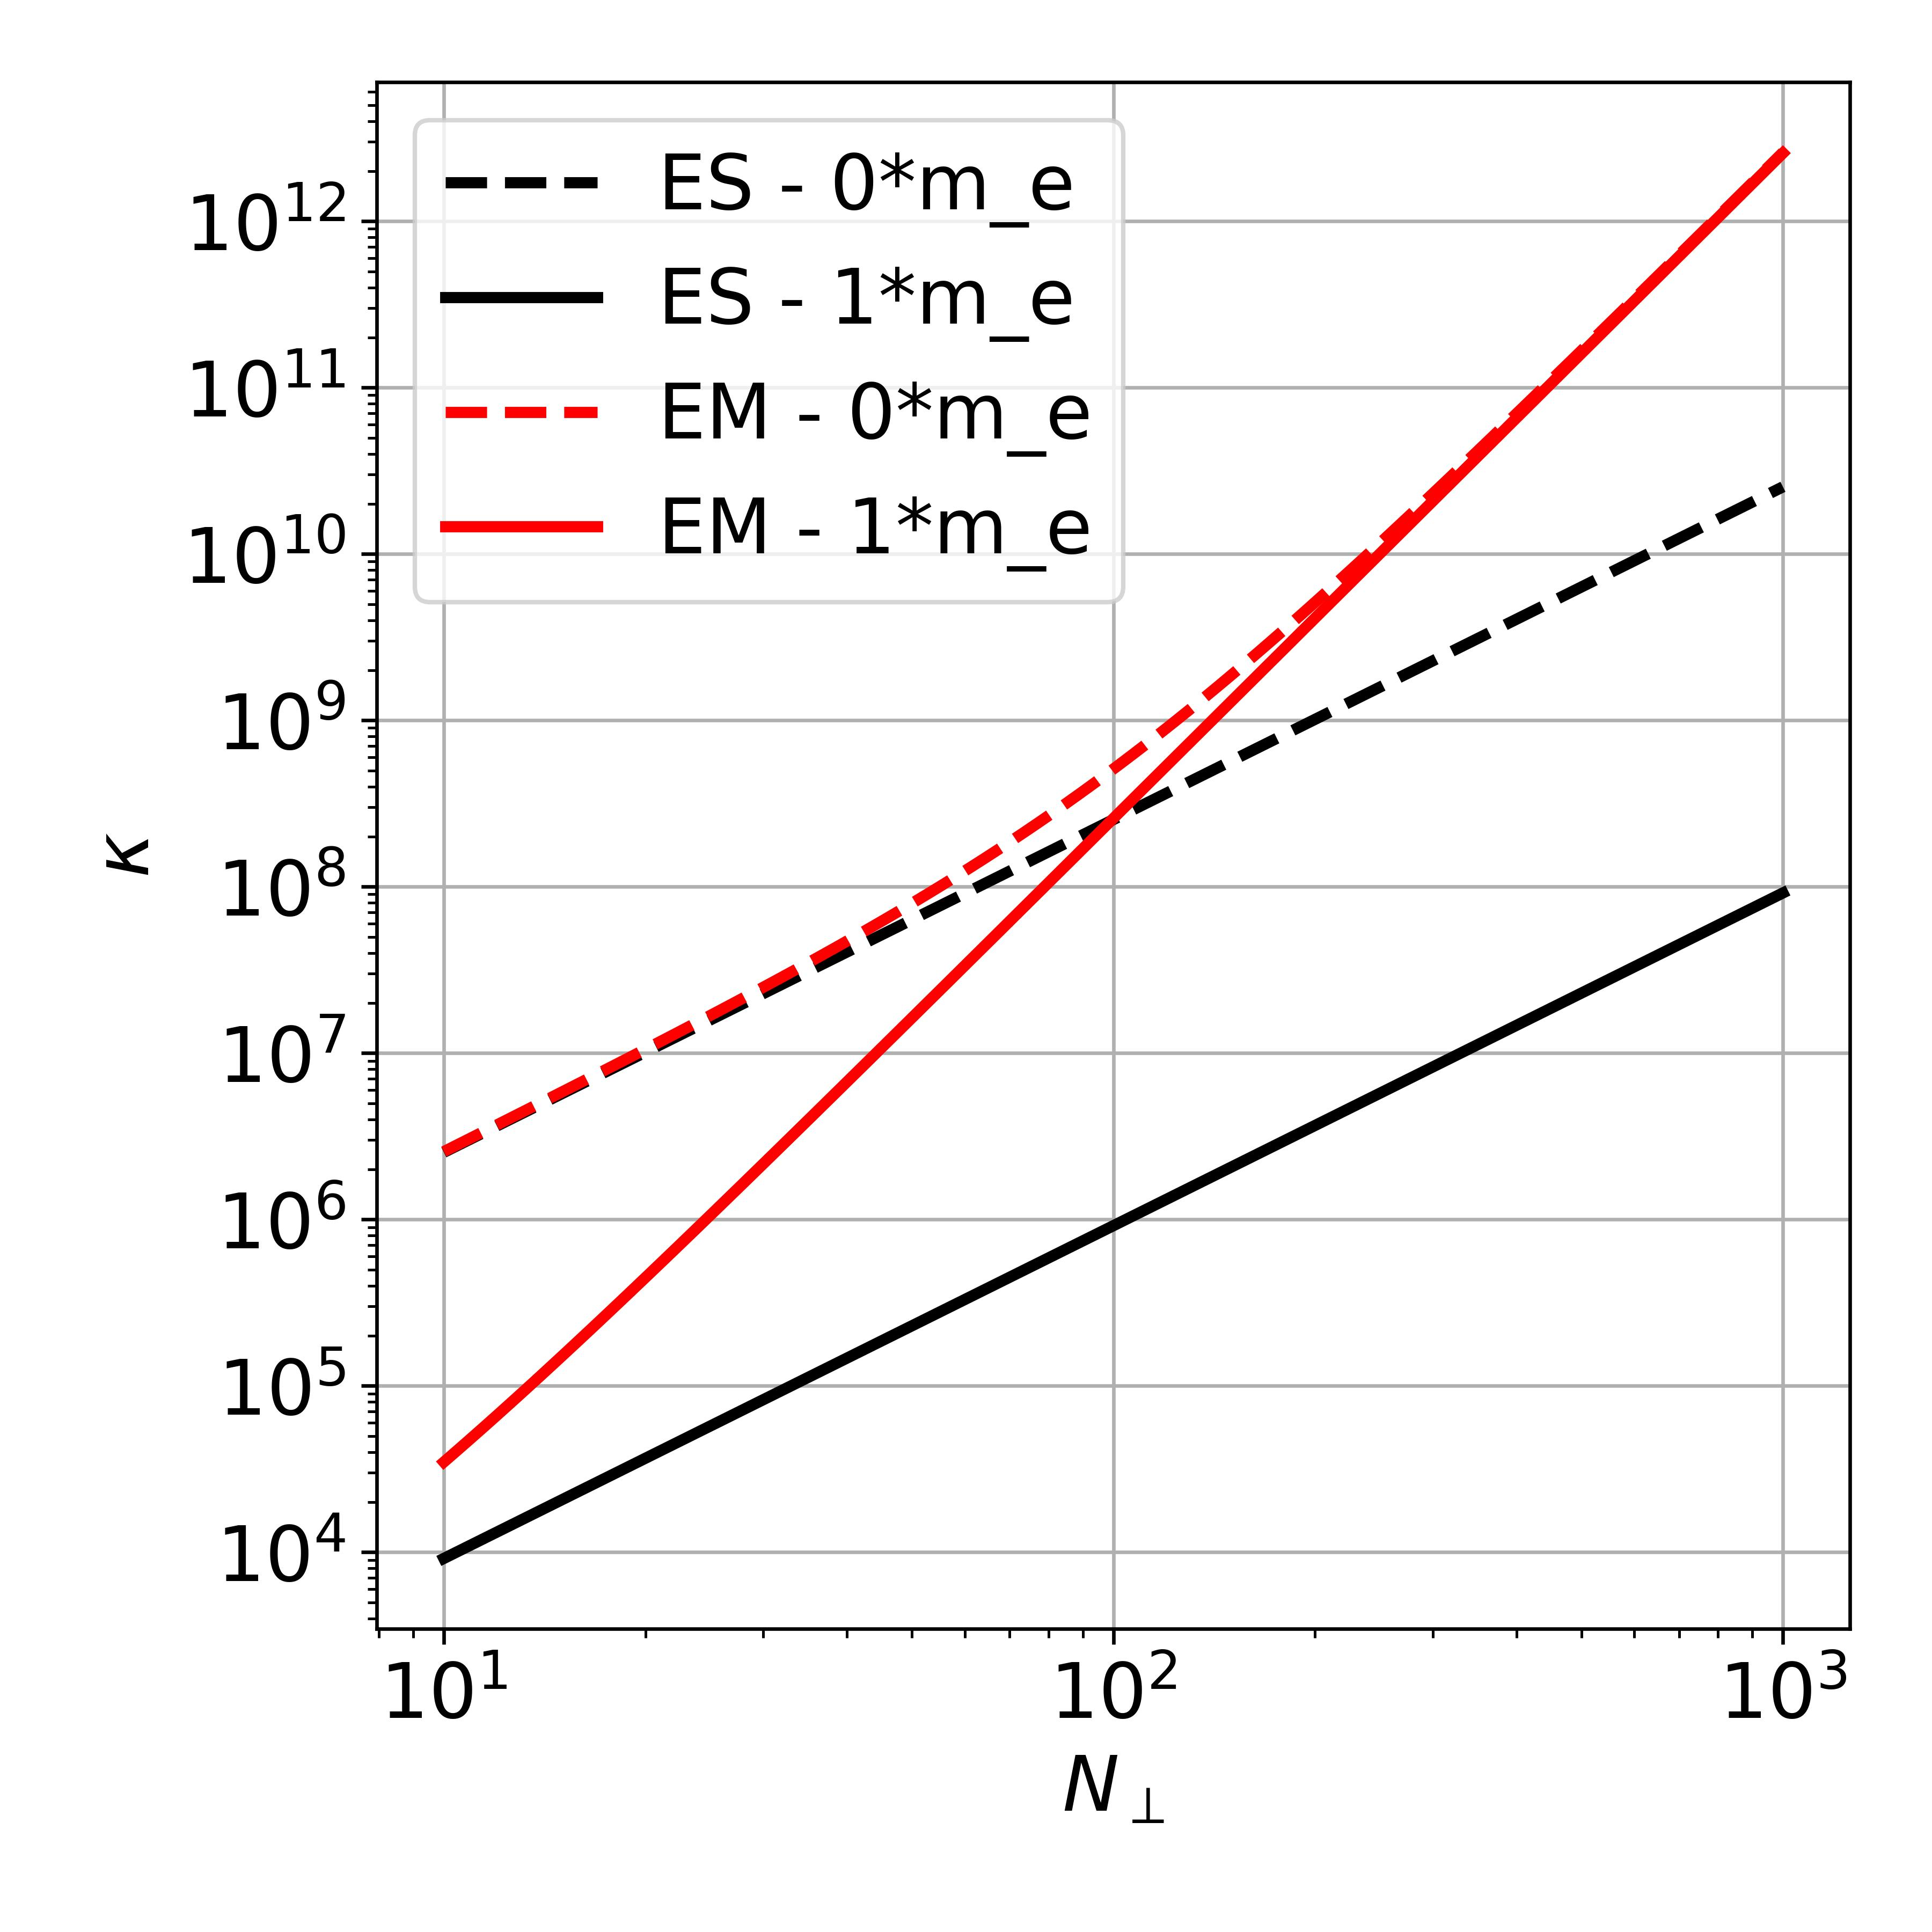
\includegraphics[width=1\textwidth]{schemes/conditionNumber_Nperp.jpg}
		\subcaption{Perpendicular \\ resolution $N_\perp$}
		\label{fig:Impl_conditionNumber_Nperp}
	\end{subfigure}
	\caption[Impact of different parameters on the condition number]{Impact of different parameters on the condition number. Plasma parameters are taken as constant: $B=1$, $m_i = 2$, $n_e = n_i = 2$, $m_e = 5.5\cdot 10^{-4}$, $\beta_0 = 10^{-3}$, $\eta_\parallel = 10^{-6}$, $\delta_t = 1$ and $N_\perp = 100$. The parameters $\beta_0$ and $n_e$ are deliberately chosen large to ensure the validity of the positive-definiteness condition \ref{eq:Impl_conditionPositiveDefinite}. Black curves correspond to the electrostatic system, and red curves to the electromagnetic matrices, with full lines indicating electron inertia and dashed lines representing $m_e = 0$.}
	\label{fig:Impl_conditionNumber}
\end{figure}

Overall, electromagnetic models exhibit a higher condition number. In particular, at larger timestep sizes or higher perpendicular resolutions, $\kappa$ increases significantly due to the third and fourth exponents in the second term of Eq. \ref{eq:Impl_conditionNumberElectromagneticVorticitySystem}. However, electron inertia positively affects the condition number. This is especially evident as $\eta_\parallel$ approaches zero in Fig. \ref{fig:Impl_conditionNumber_eta}, where neglecting the electron mass results in a sharp increase in $\kappa$, while electron inertia allows for a stable, low $\kappa$. Similarly, for low timestep sizes and resolutions, $m_e$ improves the system, such that for lower ranges, the electromagnetic system with inertia performs better than the electrostatic system without inertia.





\section{Numerical treatment of flutter}
\label{sec:impl_flutter}
In our perturbative approach, flutter introduces a radial component to the magnetic field. As the meshing remains aligned to the equilibrium field, the unit magnetic field has now an additional non-zero contravariant component $b^\psi$ in the curvilinear metric. We must hence extend all parallel operators in the code to consider it. Flutter also has a poloidal and a (small) toroidal component, but these are much less problematic to treat as they can be added to the equilibrium components:

\begin{align}
	b^\theta &= b_{eq}^\theta + \tilde{b}^\theta & b^\varphi &= b_{eq}^\varphi + \tilde{b}^\varphi
\end{align}

and the code proceeds as usual. \\ 

In this section, we describe how the radial magnetic field has been included in all parallel operators, namely in the advection scheme, the implicit diffusion problems on viscosity and heat and, crucially, the electromagnetic vorticity system.


\subsection{Radial advection}
\label{ssec:impl_flutterAdvection}

All conserved fields are advected by the total velocity. In the drift-reduced approach, it decomposes into a parallel advection along the magnetic field lines with velocity $v_\parallel=\gamma_\parallel / n$ and a perpendicular advection with the plasma drifts. Flutter then corresponds to an additional transport term at $v_\parallel$ in radial direction. For any quantity $X$, the advection term can be expressed to: 

\begin{equation}
	\grad\cdot \left[X\left(v_\parallel\mathbf{b}_{eq}+v_\parallel\tilde{\mathbf{b}} + \mathbf{u}_\perp\right)\right]
\end{equation}

In  the WENO scheme, fluxes in and out a cell are treated independently for each direction. The only novelty with flutter appears for radial fluxes, where the contravariant $v_\parallel \tilde{b}^\psi$ adds to the existing advection by $u_\perp^\psi$. Effectively, flutter acts a new drift velocity and required relatively little adaptation of the code.

\subsection{Parallel diffusion}
\label{ssec:impl_3DGunter}

In the magnetostatic setting, the parallel diffusion operator on $v_i$ and $T_\alpha$ can be solved independently on each flux surface in a 2D system on the $\theta - \varphi$ plane. The scheme developed by Günter et al. \cite{gunter2005} has proven well-suited to solve the 2D parallel Laplacian equations with minimized numerical spread for highly anisotropic problems. For an operator of the type $\nabla \cdot (\kappa \nabla_\parallel \circ \mathbf{b} )$, parallel gradients are first calculated in cell corners with finite differences and then used in the fluxes across each cell face to get the divergence. The corners where gradients are calculated are shown in Figure \ref{fig:Gunter2D}.  \\

However, with flutter (Sec. \ref{ssec:S3X_flutter}), magnetic flux surfaces are no longer aligned to the $\theta - \varphi$ plane because of the new radial component $b^\psi$. As a consequence, all independent 2D problems across flux surfaces are now coupled into a single 3D problem. For the parallel diffusion solver, a first approach would be to extend the above scheme by calculating gradients in the 3D corners of our cells. However, the new component $b^\psi$ is a pure fluctuation, which is therefore expected to be much smaller than $b^\theta$ or $b^\varphi$ and can even vanish locally. This results in significant spurious numerical diffusion in the radial direction of equilibrium gradients. To prevent this diffusion, and still properly capture radial flutter gradients, only crossed derivatives $b^\theta b^\psi$ and $b^\varphi b^\psi$ as well as the principal radial diffusion $b^\psi b^\psi$ use gradients evaluated at 3D corners, while the equilibrium diffusion remains aligned to the $\theta - \varphi$ plane. Examples of the gradients used in this new scheme are shown in Figs. \ref{fig:Gunter3D_theta} and \ref{fig:GunterD_psi}. The new discretization stencil then corresponds exactly to the equilibrium 2D stencil in the limit $b^\psi=0$. \newline

\begin{figure}[H]\centering
	\begin{subfigure}[t]{0.32\textwidth}
		\centering
		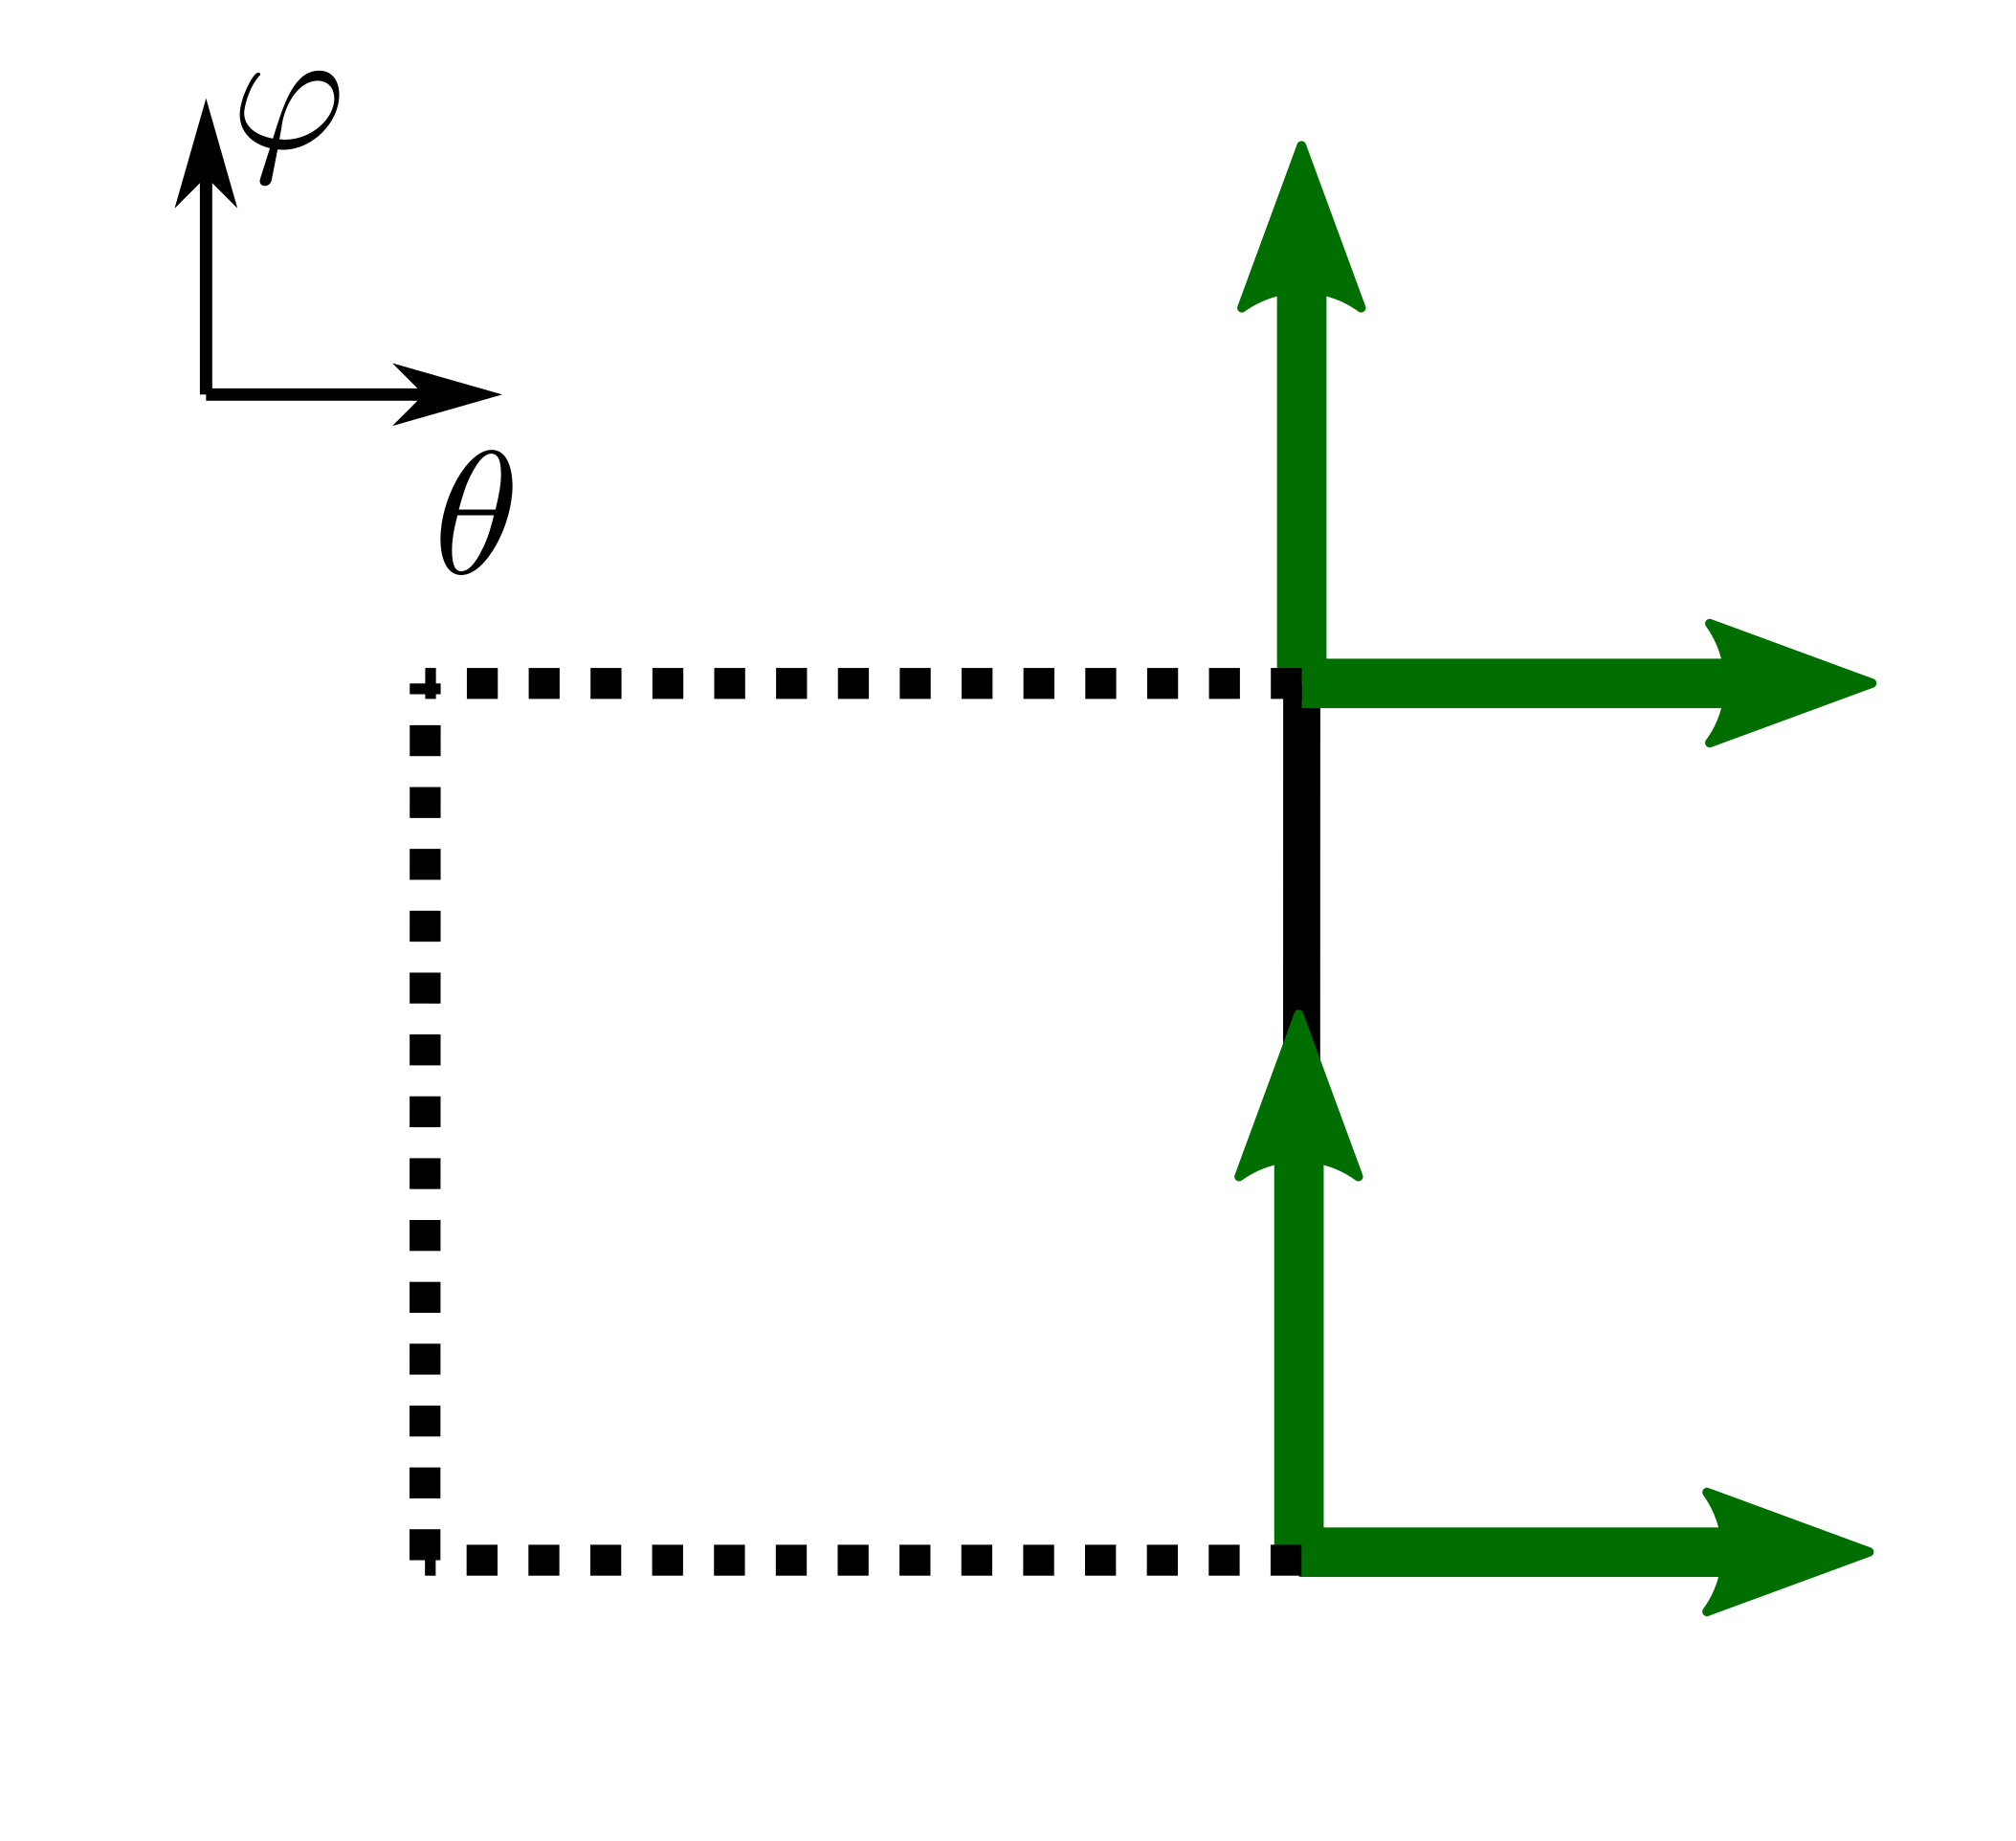
\includegraphics[width=\textwidth]{schemes/Gunter2D.png}
		\caption{ Gradients for the $\theta$-flux without flutter}
		\label{fig:Gunter2D} 
	\end{subfigure}
	\begin{subfigure}[t]{0.32\textwidth}
		\centering
		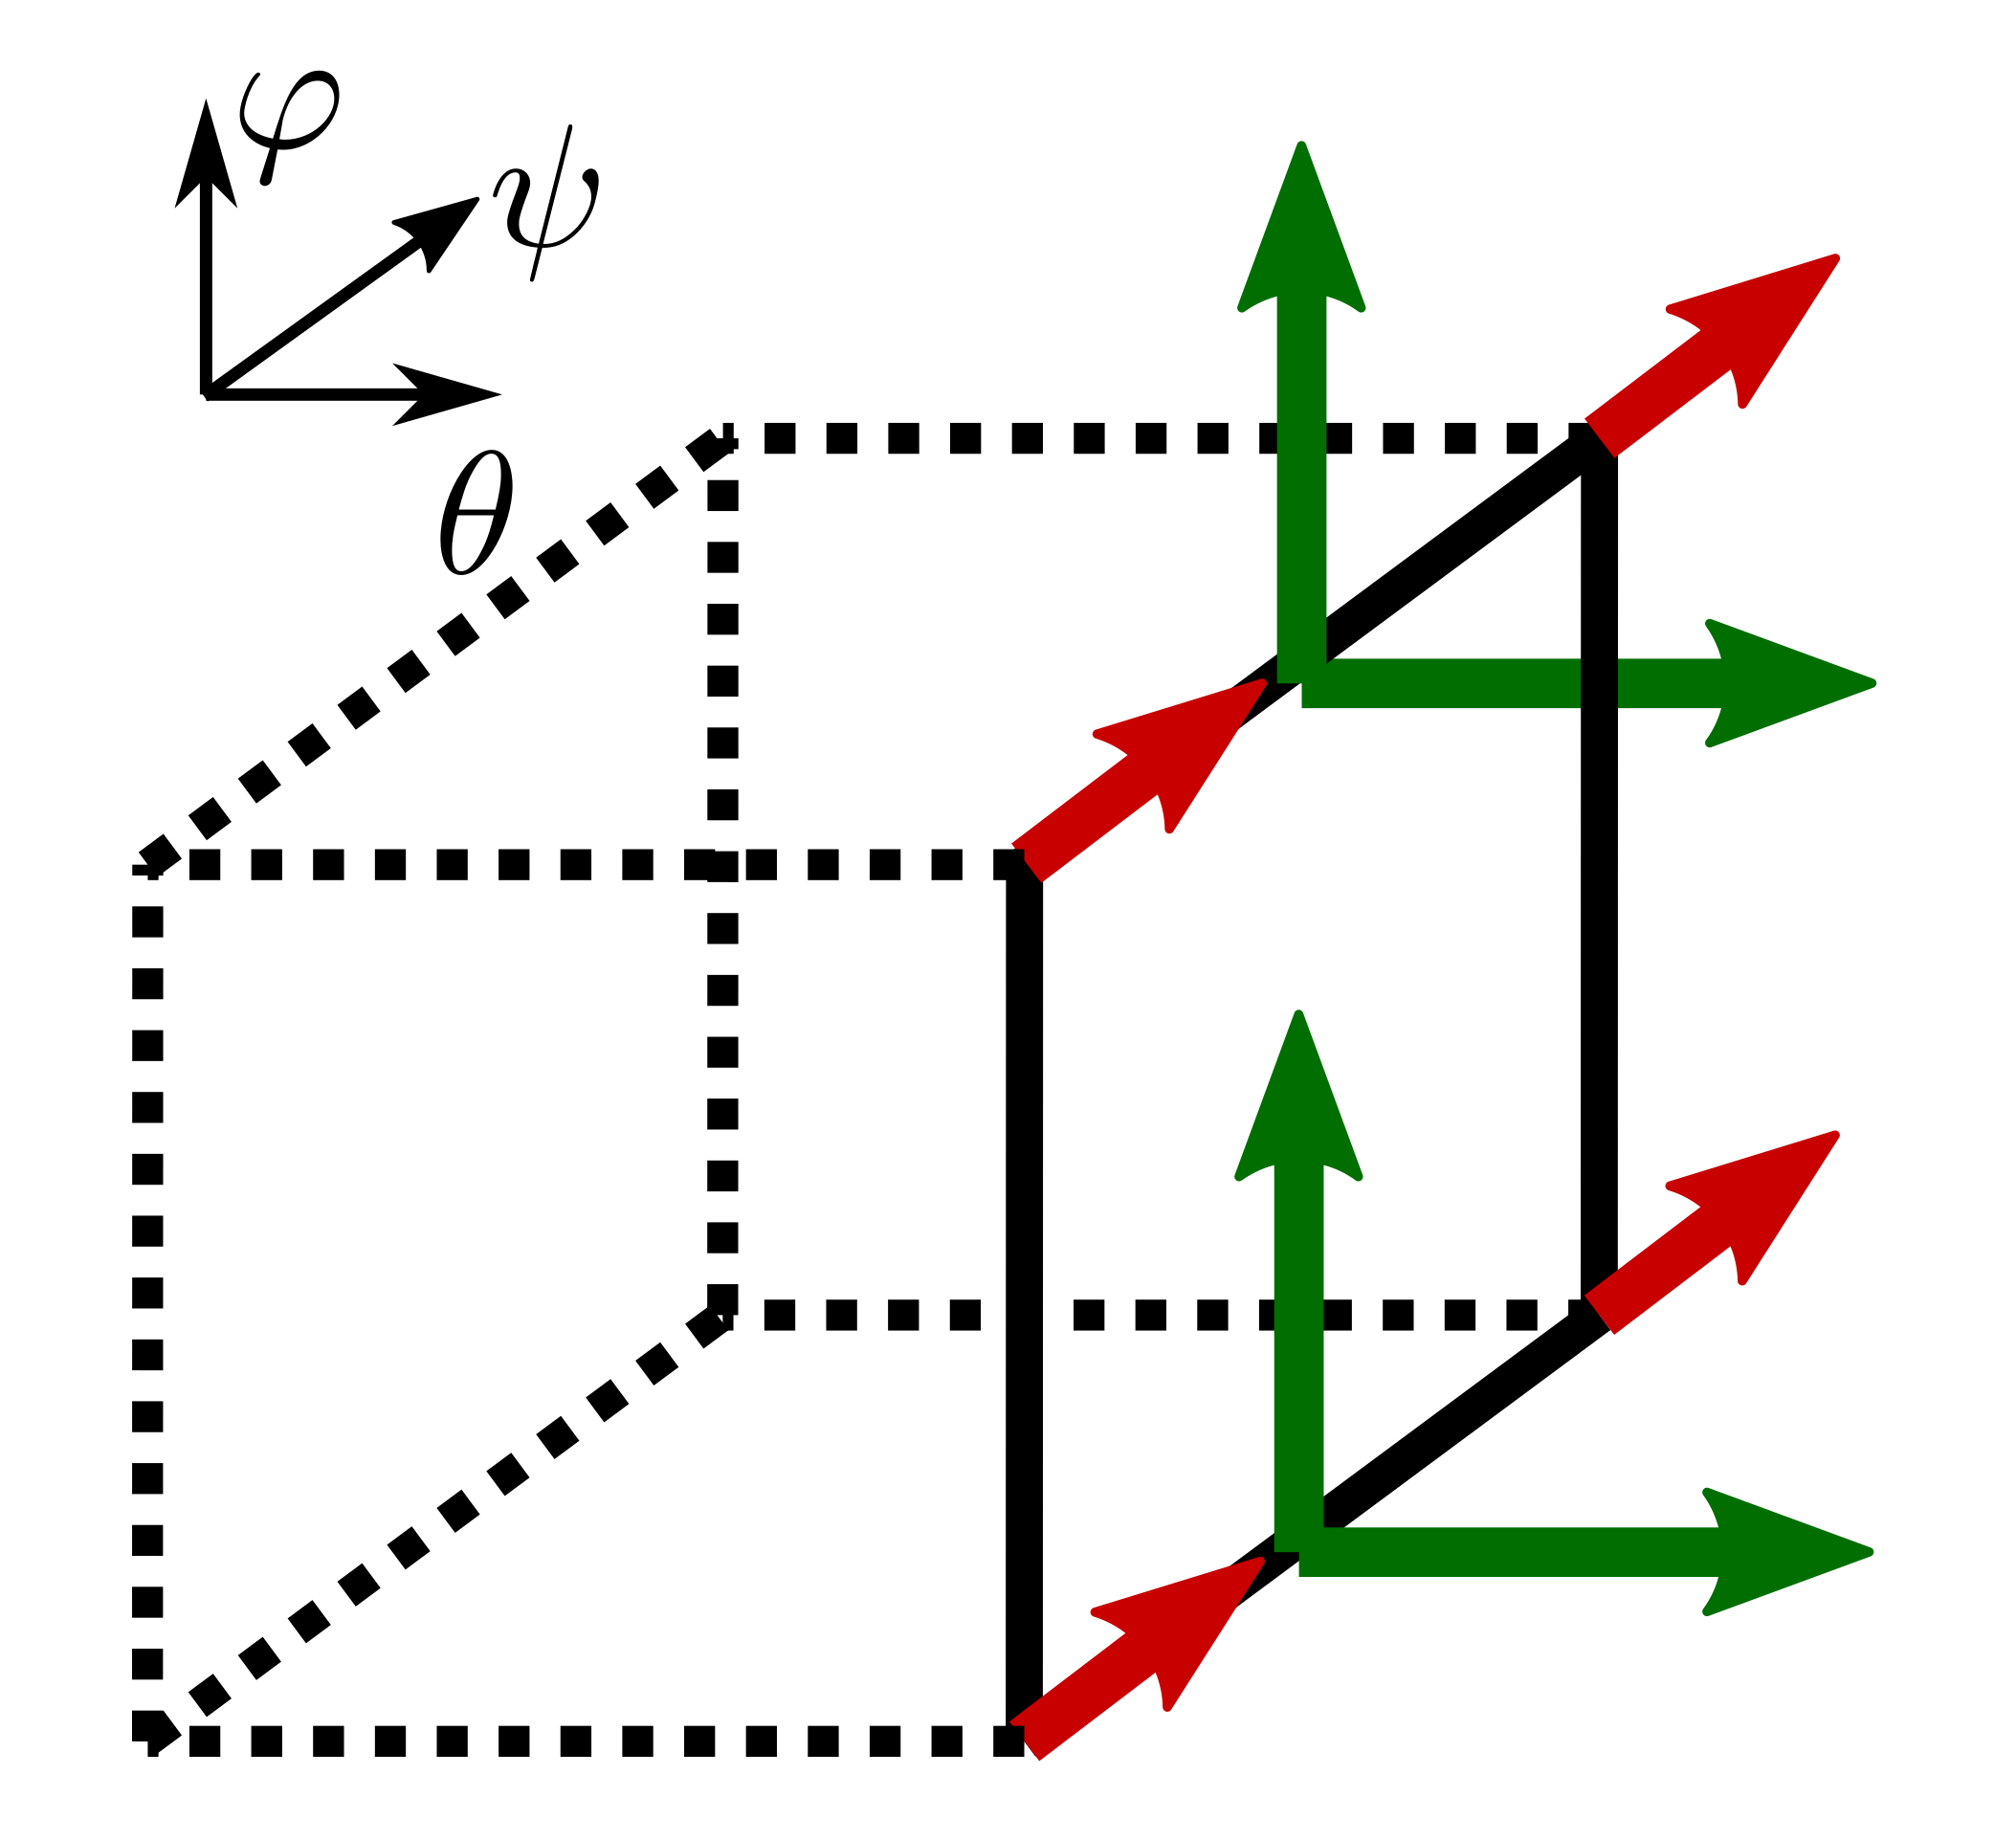
\includegraphics[width=\textwidth]{schemes/Gunter3D_theta.png}
		\caption{ Gradients for the $\theta$-flux with flutter}
		\label{fig:Gunter3D_theta} 
	\end{subfigure}
	\begin{subfigure}[t]{0.32\textwidth}
		\centering
		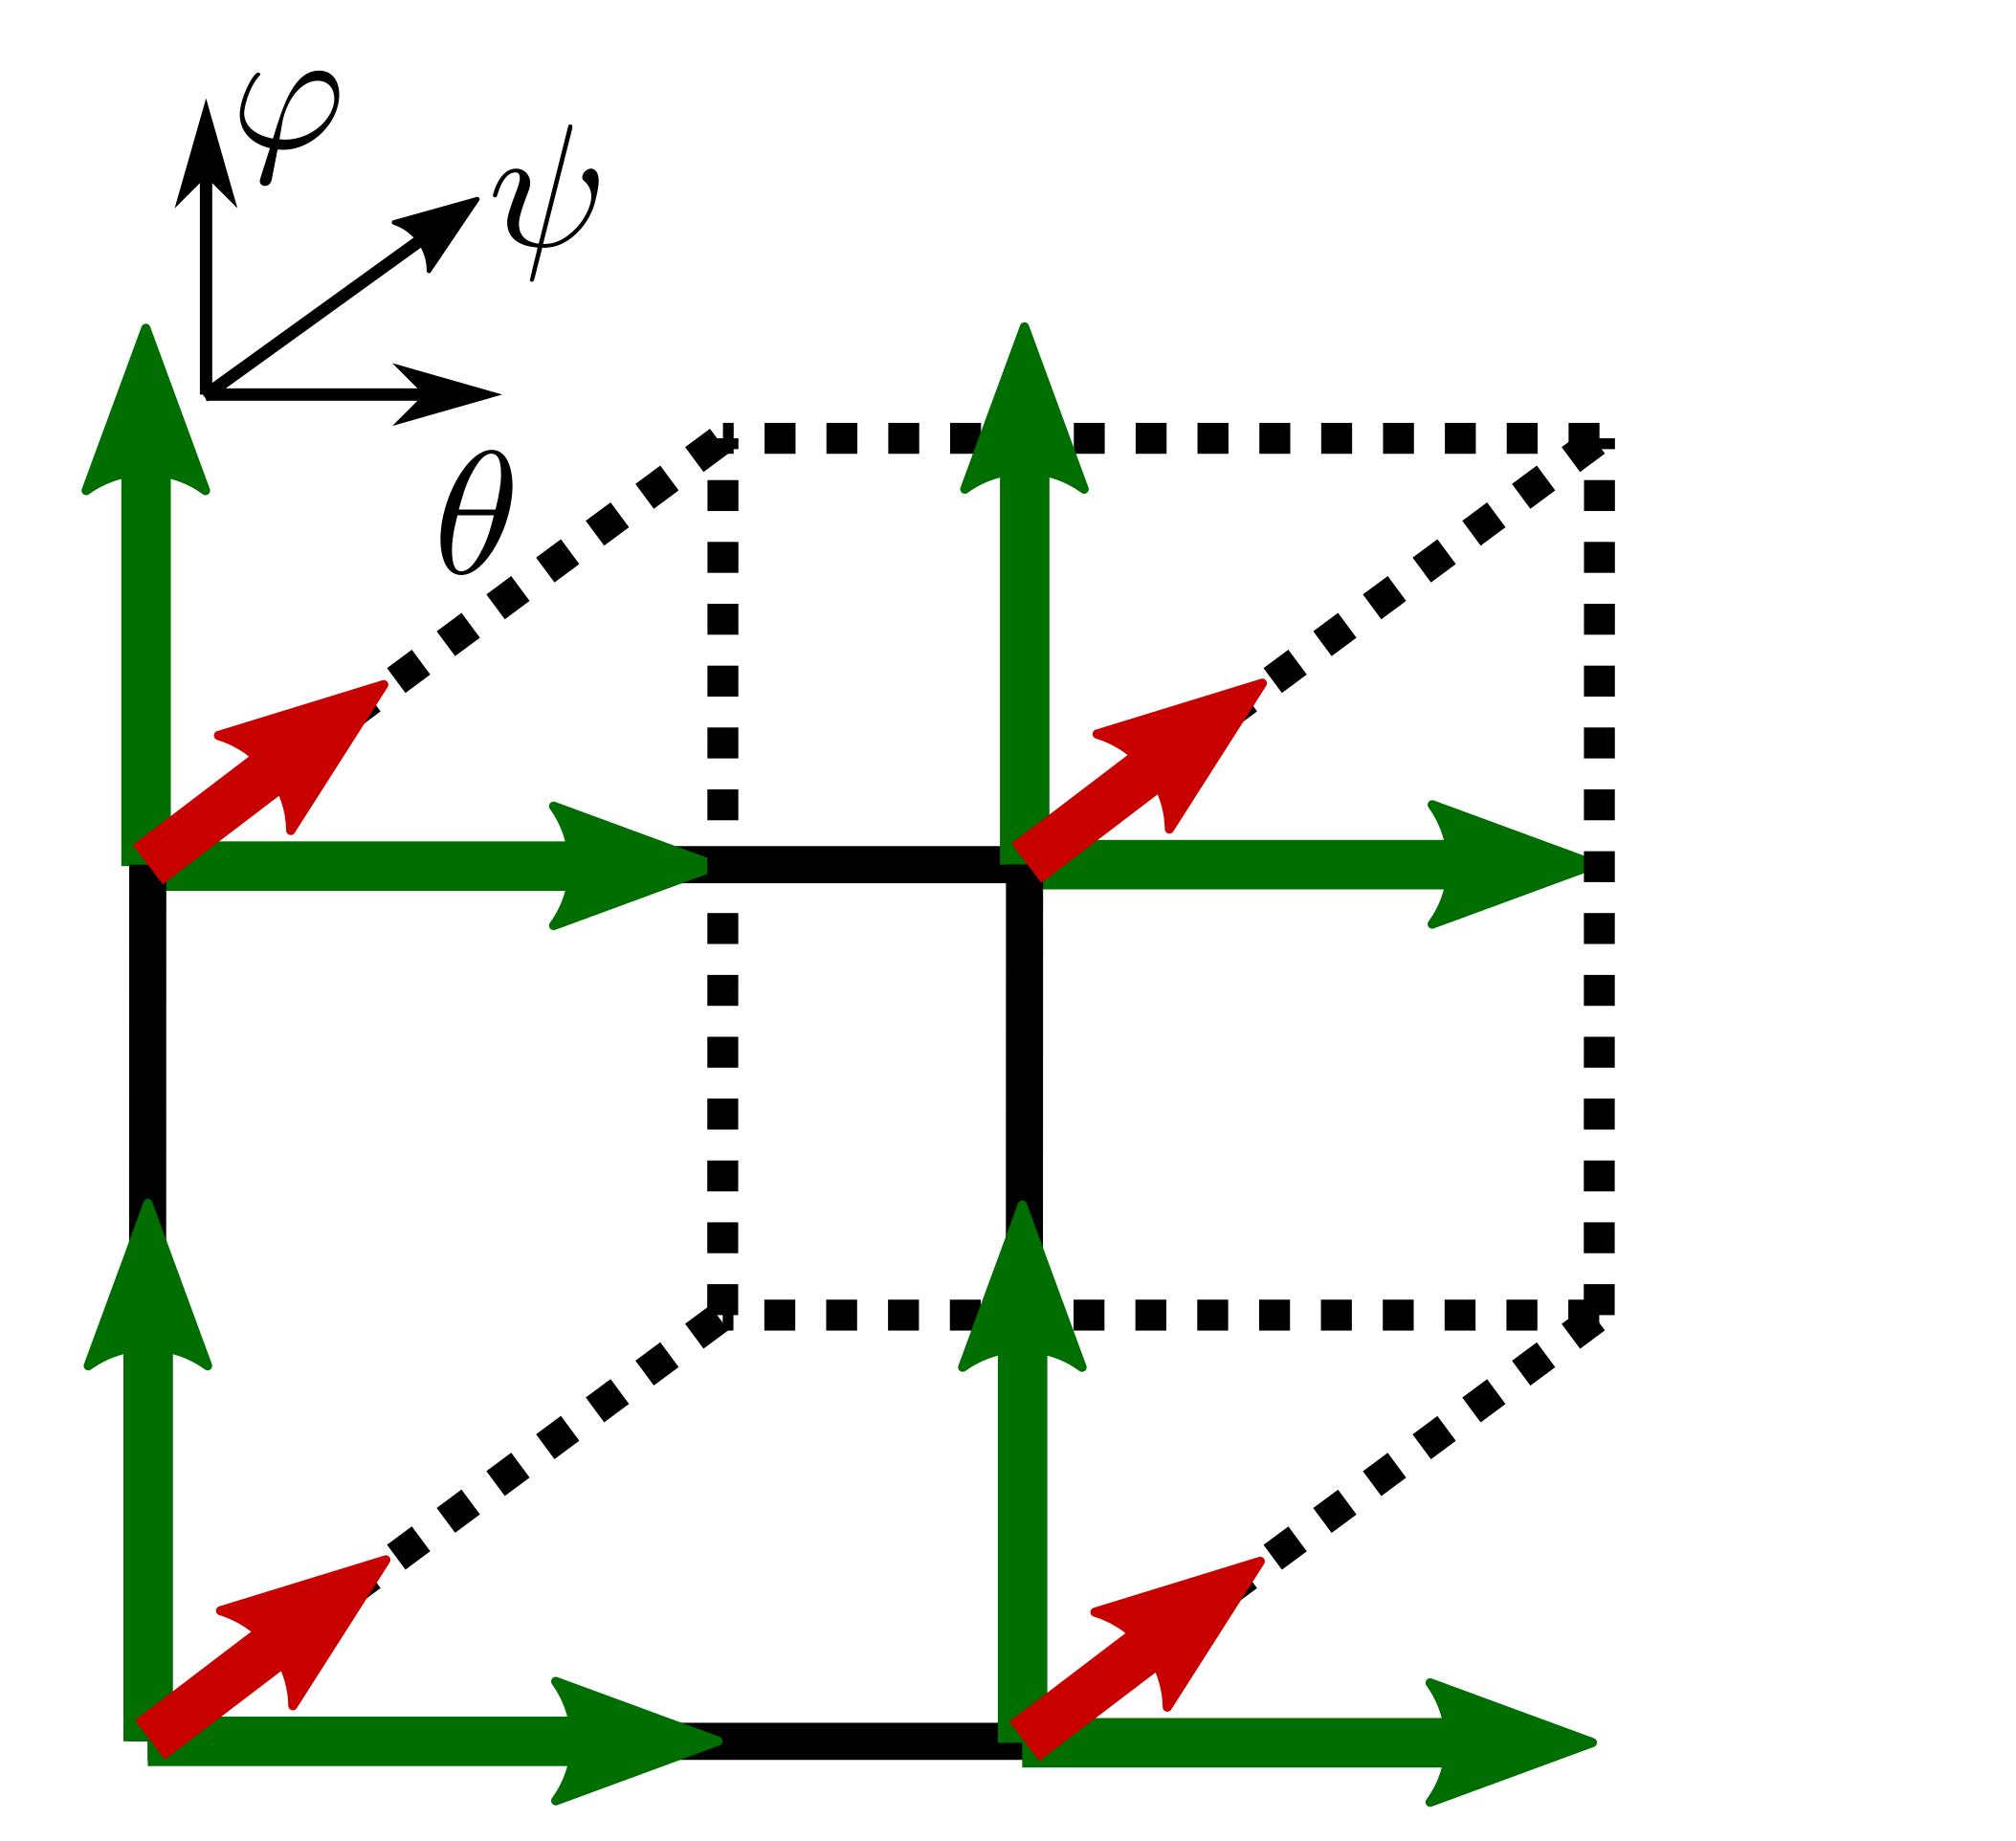
\includegraphics[width=\textwidth]{schemes/Gunter3D_psi.png}
		\caption{ Gradients for the $\psi$-flux with flutter}
		\label{fig:GunterD_psi}
	\end{subfigure}
	\caption[Sketches showing the calculation of gradients for the parallel diffusion scheme]{Sketches showing the calculation of gradients for the parallel diffusion scheme. It shows the position where the different gradients are calculated that are relevant for a flux across the cell face with a solid line. Green and red arrows symbolize gradients in the equilibrium and in the radial direction, respectively.}
	\label{fig:GunterStencils_flutter}
\end{figure}



\subsection{Vorticity equation}

For the parallel diffusion on the electric potential $\nabla \cdot \left[ D_\parallel \nabla_\parallel \Phi \mathbf{b} \right]$ with flutter, we do not use the stencil introduced in Sec. \ref{ssec:impl_3DGunter}. To avoid numerical difficulties and the appearance of unphysical modes, the discretization of this term needs to be consistent with the parallel gradient and divergence operators in the same system. Since the grid for $A_\parallel$ and $j_\parallel$ is only staggered in the $\theta$ and $\varphi$ directions, we do not know them in the radial corners from Figs. \ref{fig:Gunter3D_theta} and \ref{fig:GunterD_psi}. Instead, the discrete diffusion operator is defined as the combination of the operators for the gradient and the divergence. It involves two neighbors on both radial sides, so the resulting stencil is less compact but consistent with the remaining system. Note that in cases without flutter ($b^\psi = 0$), the diffusion operator exactly corresponds to Günter's scheme \cite{gunter2005} because the staggered fields are known at the corners of the gradients in Fig. \ref{fig:GunterStencils_flutter}. \\

Generally spoken, Combining a divergence with a gradient stencil to form a discrete Laplacian is a bad idea. The information for the finite differences scheme stems from two cells away, skipping the intermediate cell. The decoupling between even and odd grid points is prone to high-frequency oscillations and  formation of a checkerboard pattern. This behavior is evident if one looks at the stencil neighbors for the Laplacian on a Cartesian grid in Fig. \ref{fig:impl_vorticityLaplStencilFlutter}, where all mixed derivatives vanish.

\begin{figure}[H]\centering
	\centering
	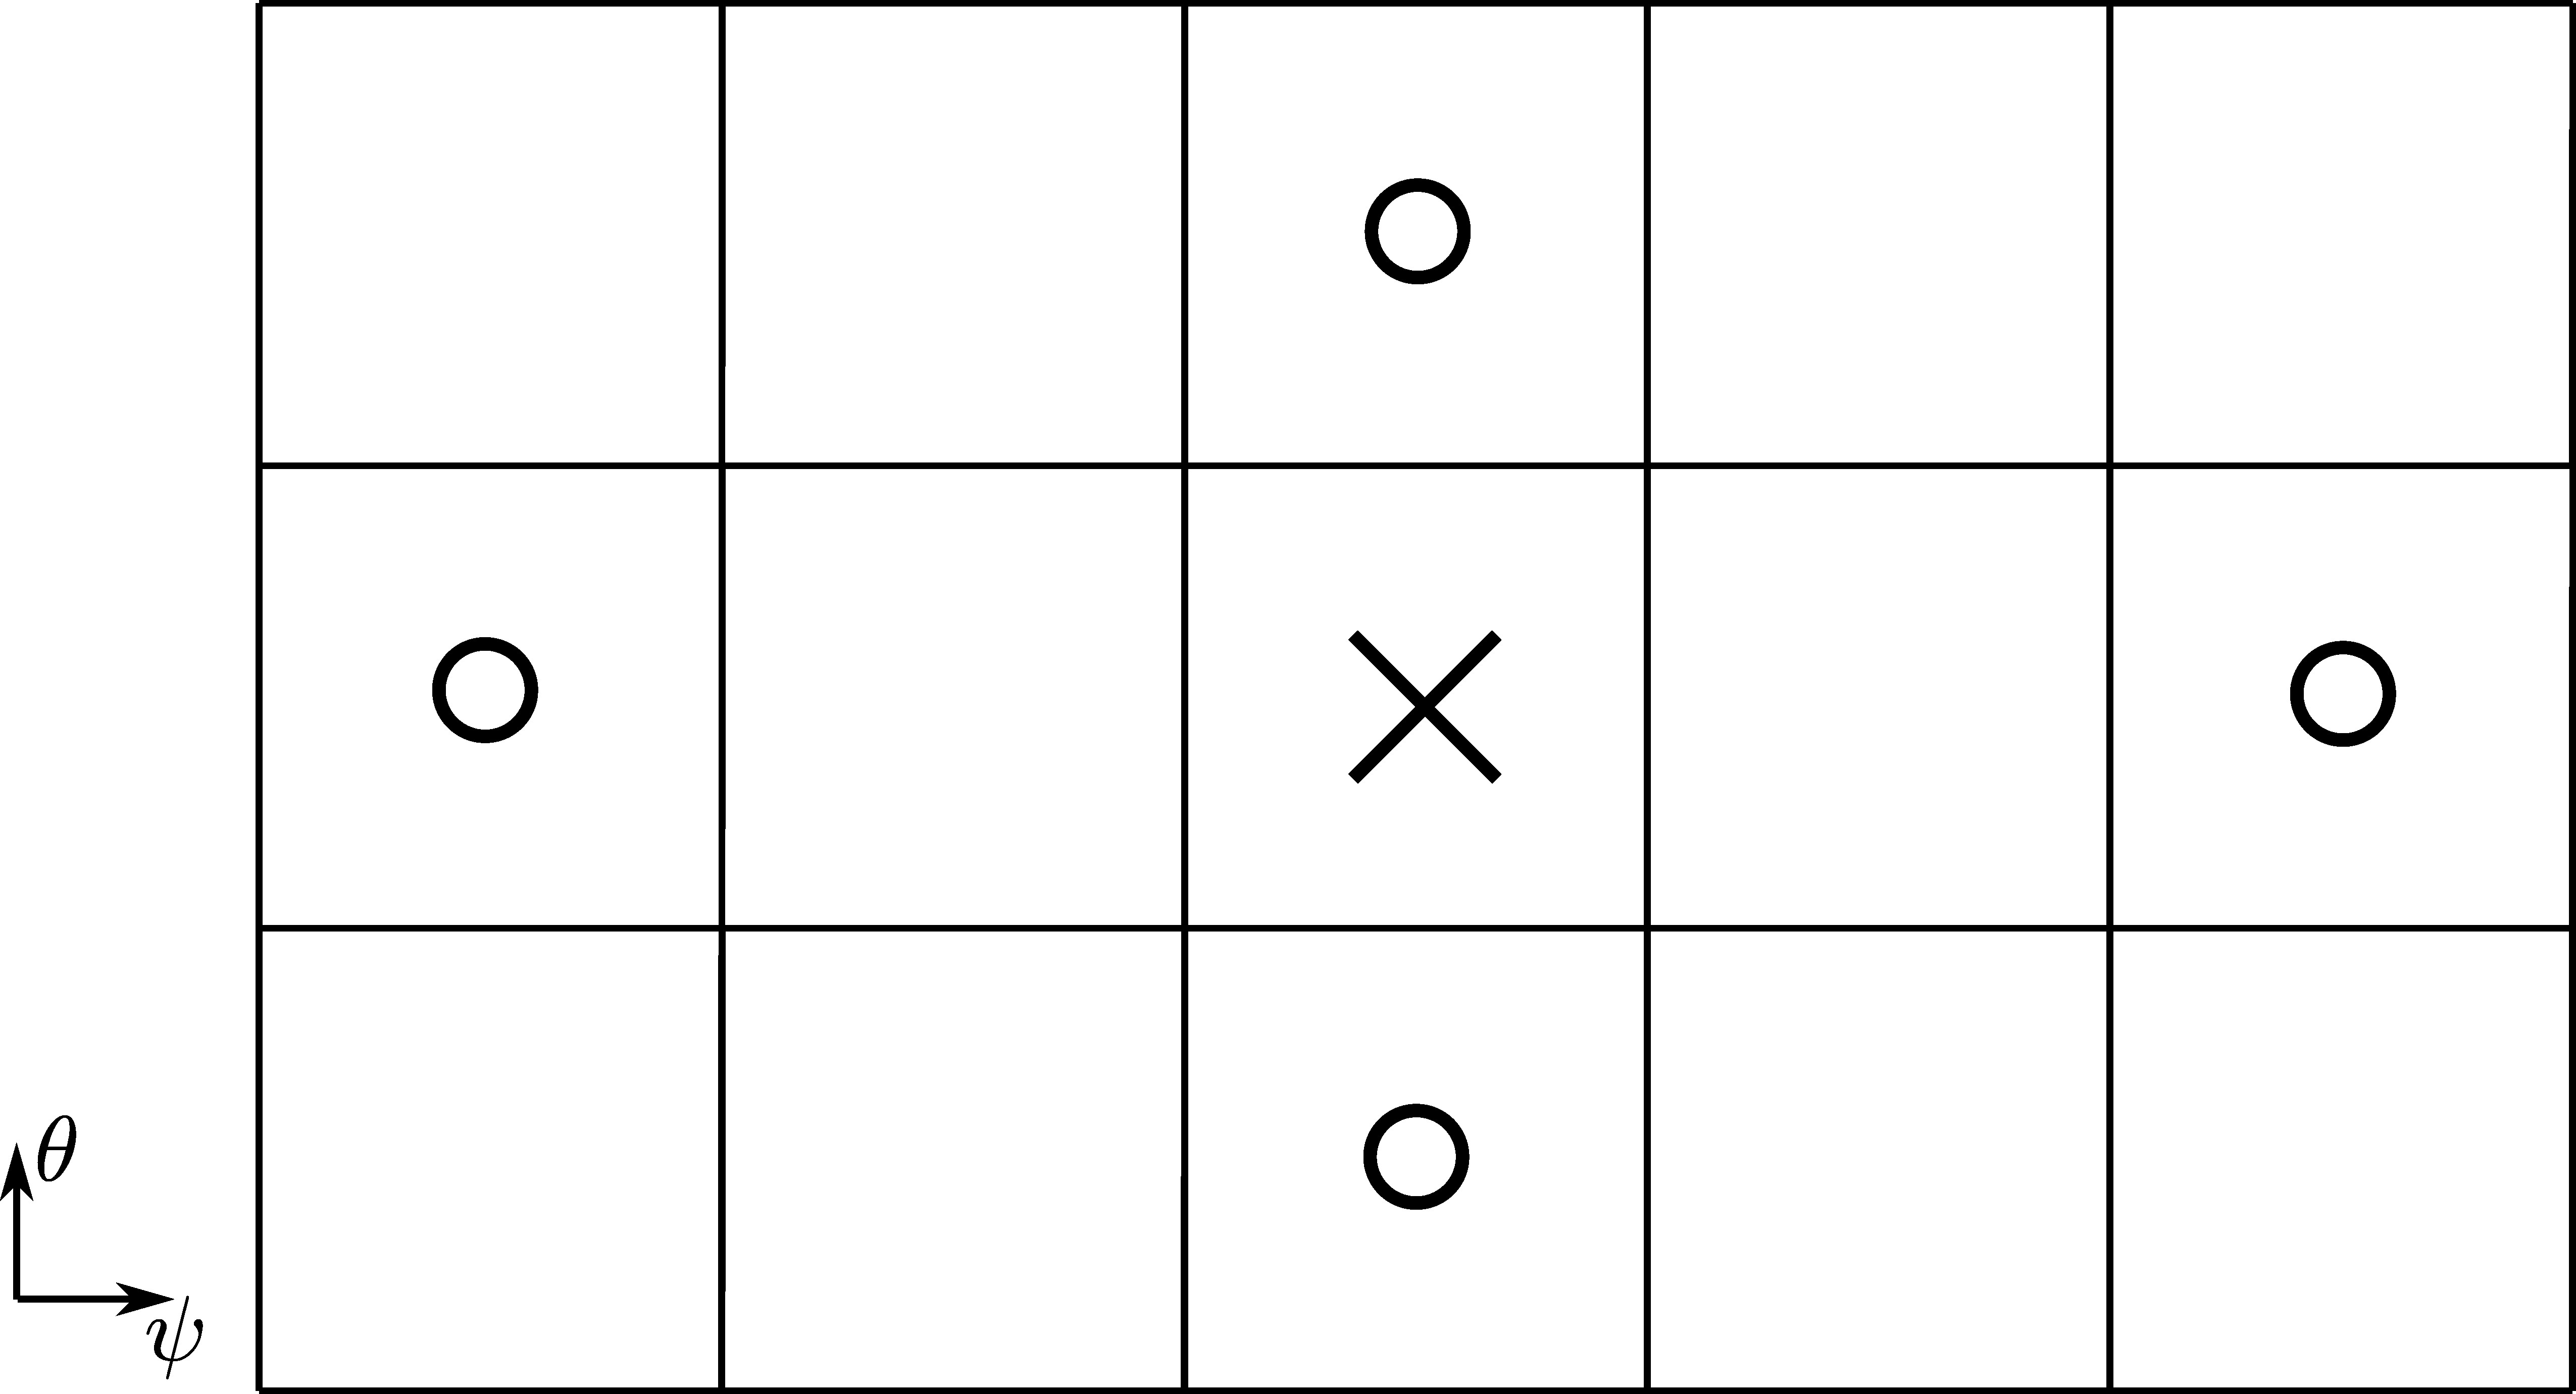
\includegraphics[width=0.6\textwidth]{schemes/vorticityLaplacianStencilFlutter.jpg}
	\caption[Neighbors of the parallel Laplacian stencil with flutter for the vorticity equation]{Neighbors of the parallel Laplacian stencil with flutter for the vorticity equation}
	\label{fig:impl_vorticityLaplStencilFlutter}
\end{figure}

For the specific application in the vorticity equation, checkerboards are not at risk to appear, because the radial component in the parallel stencil is superseded with the perpendicular Laplacian on $\Phi$ from the polarization current that considers direct neighbors, which smoothens any high-frequency modes at the resolution. Conversely, it is impossible to run stable simulations with the "better" parallel diffusion stencil with flutter from Sec. \ref{ssec:impl_3DGunter}, as it does not preserve consistency between the diffused $\Phi^n$ and $\Phi^{n-1}$. The potential $\Phi^{n-1}$ from the previous timestep enters the system through the divergence of $\partial_t j_\parallel$, whose time discretization relies on $j_\parallel^{n-1}$, and as such on $\grad_\parallel \Phi^{n-1}$. Note that this reasoning also applies for the parallel Laplacians on $\log n_e$ and $T_e$ that appear in the right-hand side of the vorticity equation and are important for the non-adiabatic plasma response. 
 





